\documentclass{ieeeaccess}
\usepackage{cite}
\usepackage{amsmath,amssymb,amsfonts}
\usepackage{algorithmic}
\usepackage{graphicx}
\usepackage{stfloats}
\usepackage{subfigure}
\usepackage{float}
\usepackage{multirow}
\usepackage{multicol}
\usepackage{enumitem}
\usepackage{xcolor}
\usepackage{romannum}% for approach #1 and #2




\usepackage{textcomp}
\def\BibTeX{{\rm B\kern-.05em{\sc i\kern-.025em b}\kern-.08em
    T\kern-.1667em\lower.7ex\hbox{E}\kern-.125emX}}
\begin{document}
\history{Date of publication xxxx 00, 0000, date of current version xxxx 00, 0000.}
\doi{10.1109/ACCESS.2017.DOI}

\title{DANS: Deep Attention Network for Single Image Super-Resolution}
\author{\uppercase{Jagrati Talreja}\authorrefmark{1}, \IEEEmembership{Graduate Student Member, IEEE},
\uppercase{SUPAVADEE ARAMVITH}\authorrefmark{2},\IEEEmembership{Senior Member, IEEE}, AND
\uppercase{Takao Onoye }\authorrefmark{3},
\IEEEmembership{Senior Member, IEEE}}
\address[1]{Department of Electrical Engineering, Faculty of Engineering, Chulalongkorn University, Bangkok 10330, Thailand.}
\address[2]{Multimedia Data Analytics and Processing Unit, Department of Electrical Engineering, Faculty of Engineering, Chulalongkorn University, Bangkok 10330, Thailand.}
\address[3]{Graduate School of Information Science and Technology, Osaka University, 1-5 Yamada-Oka, Suita, 565-0871 Japan}
\tfootnote{This research is funded by the Second Century Fund (C2F), Department of Electrical Engineering, Faculty of Engineering, Chulalongkorn University Bangkok, 10330, Thailand. This research is also funded by Thailand Science Research and Innovation Fund Chulalongkorn University (CU\textunderscore FRB65\textunderscore ind (9)\textunderscore 157\textunderscore 21\textunderscore 23), The NSRF via the Program Management Unit for Human Resources \& Institutional Development, Research and Innovation [grant number B$04G640053$] and also funded by Thailand Science research and Innovation Fund Chulalongkorn University (IND$66210019$). } \markboth
{Author \headeretal: Preparation of Papers for IEEE TRANSACTIONS and JOURNALS}
{Author \headeretal: Preparation of Papers for IEEE TRANSACTIONS and JOURNALS}

\corresp{Corresponding author:  Supavadee Aramvith (supavadee.a@chula.ac.th).}

\begin{abstract}
The current advancements in image super-resolution have explored different attention mechanisms to achieve better quantitative and perceptual results. The critical challenge recently is to utilize the potential of attention mechanisms to reconstruct high-resolution images from their low-resolution counterparts. This research proposes a novel method that combines inception blocks, non-local sparse attention, and a U-Net network architecture. The network incorporates the non-local sparse attention on the backbone of symmetric encoder-decoder U-Net structure, which helps to identify long-range dependencies and exploits contextual information while preserving global context. By incorporating skip connections, the network can leverage features at different scales, enhancing the reconstruction of high-frequency information. Additionally, we introduce inception blocks allowing the model to capture information at various levels of abstraction to enhance multi-scale representation learning further. Experimental findings show that our suggested approach produces superior quantitative measurements, such as peak signal-to-noise ratio (PSNR), structural similarity index (SSIM), visual information fidelity (VIF), and visually appealing high-resolution image reconstructions. 
\end{abstract}

\begin{keywords}
Image super-resolution; Inception blocks; Non-Local Sparse Attention; U-Net.
\end{keywords}

\titlepgskip=-15pt

\maketitle

\section{Introduction}
\label{sec:introduction}
\PARstart{I}n convolutional neural network-based image processing, single image super-resolution (SISR) is one of the most important research fields. Super-Resolution (SR) is a classified modern-day problem needing immediate solutions. All the vision task-based devices require embedding fast and less complex Super-Resolution (SR) algorithms for faster and high-quality processing of visuals, i.e., images, videos, or live streaming. Focusing on images, the SR appertains to recuperating high-quality images from given low-quality images, and this process is termed Image Super-Resolution (ISR). 
SISR is an ill-posed problem because of the generation of multiple High-Resolution (HR) images corresponding to a single Low-Resolution (LR) image. Due to this reason, detailed constraints of images such as high-frequency, low-frequency, spatial characteristics, or a variety of image priors and domains are used as features of an image. These insightful and hierarchical features recover the finer detail of any image, which further helps in security and surveillance and many other vision-based applications such as image segmentation [1, 4], reconstruction [2], estimation [3],  object and anomaly detection [5], etc. having varied applicability in security, surveillance [6], medical [7], face [8, 9], satellite imaging [10], remote sensing [11].
Learning-based algorithms have recently shown remarkable performance compared to conventional super-resolution methods. Convolutional neural networks (CNN) dominate the culture for modeling the algorithms in Deep Learning (DL) [12, 13, 14, 15, 16]. The introduction of neural networks (NN) in Super-Resolution Convolution Neural Networks (SRCNN) [17] proposed by Dong \textit{et al}. has led to many advancements in the field of SISR. After the SRCNN approach, the research community explored ISR regarding model frameworks, up-sampling methods, network design, learning strategies, etc. Introducing CNNs [17], Generative Adversarial networks (GANs) [18], attention mechanisms [19, 20], transformative discriminative networks [21], and residual networks [22] has significantly improved the quality of LR images. To reduce the computational cost and training complexity, Wavelet-SRNet [23] and Deep wavelet super-resolution (DWSR) [24] were the first to super-resolve images in the wavelet domain, which uses the contextual information of an image by using low and high-frequency sub-bands having topological information. 
Fan \textit{et al}. [25] concluded the favorability of sparsity [26, 27] constraints by imposing sparsity [28] and proved the increase in efficiency of neural networks [29]. Meanwhile, with network architecture, development turned towards exploring the sparsity constraints using attention mechanisms in sequential models. It emerged as a top-tier standard for Peak Signal-to-Noise ratio (PSNR) or Structural Similarity Index Measure (SSIM). Non-Local Sparse attention (NLSN) [30] is one of the most efficient current examples of a non-local channel attention-based sequential model for getting structural information in dominant or more focused regions. However, there is room for improving computational efficiency and reconstruction of finer details while preserving the natural textures of this sequential model. 

Considering the current scenario of fast processing smart edge devices or embedded systems on chip (SoC), the model size must be considered for achieving faster and state-of-the-art (SOTA) comparable outcomes for higher and arbitrary enlargement factors. Several enhancements in ISR are based on sequential model designs. In this experiment, research work showed higher
performance gains with reduced model size. Even though the sequential model helps to improve the network performance, they still face some limitations.

(1) Above mentioned methods are computationally expensive and require substantial processing power and time. They also require storing and accessing large affinity matrices demanding significant memory resources.
(2) These methods can sometimes introduce unwanted artifacts or distortions into super-resolved images. The artifacts can include checkboard patterns, jagged edges, or blurring in certain regions.
(3) When the input image is extremely low-resolution and contains noise or compression artifacts, earlier methods can struggle to recover fine details or remove noise patterns effectively.

An efficient way to overcome all those problems is to combine the sequential models [30] with non-sequential models [4]. The non-sequential methods have been proven to achieve meaningful features and effectively capture regional and global image subjects. Furthermore, this approach [30] helps to address the information loss encountered in deep neural networks. Isola \textit{et al}. [31] first considered sequential models as encoder-decoder networks [32] and linked them with non-sequential architectures to separate high and low-frequency components of an image. Working with the same approach, we propose a novel approach for image super-resolution that combines non-local sparse attention with a U-Net network architecture and integrates inception blocks. The U-Net architecture serves as the backbone of our proposed network architecture. The skip connections [33] and encoder-decoder [32] structure enable efficient feature learning at various scales. The non-local sparse attention module enables the network to capture long-range dependencies by modeling the correlations between image patches and enhancing information exchange across the image, leading to improved utilization of contextual information for SR reconstruction.  The integration of skip connections [34] ensures that the network can leverage features from different layers, enabling the efficient recovery of high-frequency information. To further enhance multi-scale representation learning, we introduce inception blocks into our network architecture, enabling the model to capture information at various levels of abstraction. This enriches the network's capability to capture local and global structures, enhancing super-resolution performance.
In summary, the main contributions of our proposed model are listed below:
(i)	Propose a non-sequential backbone with skip connection to enable efficient feature learning at different scales and reconstruction of fine image details while maintaining global context.
(ii)	Integrate the non-local sparse attention module to capture long-range dependencies, enhance information exchange across image patches and improve utilization of contextual information for SR reconstruction.
(iii)	Employ inception block and benefit from parameterized and efficient feature extraction to enhance the network capability to capture local and global structures at different levels of abstraction.
The remaining article comprises Section II, which briefly reviews the relevant work of the proposed method, and Section III describes the methodology of the network. Section IV presents the experimental results and comparative analysis with state-of-the-art methods. Discussion and Conclusion with future work are in sections V and VI.

\section{RELATED WORK}
Image super-resolution (ISR) is a well-studied problem in computer vision, and numerous techniques have been proposed to tackle the challenge of reconstructing high-resolution images from low-resolution inputs. This section provides an extensive overview of the related work in image super-resolution, focusing on deep learning-based methods, attention mechanisms, and network architectures.
Deep learning-based approaches have revolutionized the field of image super-resolution by harnessing the representation power of convolutional neural networks (CNNs). Dong \textit{et al}. introduced the pioneering work of Super-Resolution Convolutional Neural Network (SRCNN) [17], which directly utilized a shallow network to learn the mapping from low-resolution to high-resolution images. SRCNN achieved impressive results and laid the foundation for subsequent research in deep learning-based SR techniques.
Deeper and more complex network architectures have been proposed to improve SR performance. For instance, Very Deep Super-Resolution (VDSR) [35] introduced a deeper network using a 20-layer residual network. The residual learning framework allowed VDSR [35] to efficiently capture residual information and achieve state-of-the-art results at that time. After this, many methods were employed, such as Deeply Recursive Network (DRCN) [36], but it shows slow training convergence. To extend this Residual Encoder-Decoder Network (REDNet) [37] was used to enhance model performance and fasten the convergence. To further speed up the training convergence of these models, Denoising Convolutional Neural Network (DnCNN) [38] was introduced by Chen \textit{et al}. Since these deeper networks could not perform on small edge devices, the concept of introducing lightweight models was introduced [39, 40, 41]. Deep Recursive Residual Network (DRRN) [42] by Tai \textit{et al}. and Information Multi-Distillation Network (IMDN) [39] by Hui \textit{et al}. are two examples of lightweight models.
Enhanced Deep Super-Resolution (EDSR) [22] enhanced the network architecture by increasing the network depth, utilizing residual blocks, and adopting an improved optimization strategy. EDSR [22] won the New Trends in Image Restoration and Enhancement (NTIRE) 2017 challenge on single image Super-Resolution: Dataset and Study and became a benchmark for subsequent SR models. 
After this, researchers shifted to making shallower networks and focusing on designing models with less memory consumption and computation time. For this, a Persistent Memory Network for image restoration (MemNet) [43] was introduced, which combined skip connections with CNN layers. This model was shallower compared to EDSR [22] and VDSR [35]. Multi-Scale Residual Network (MSRN) [44] by Li \textit{et al}. employed adaptive feature extraction and used hierarchical information for image SR. Some methods also improve noise in an image, such as Learning a Single Convolutional Super-Resolution Network for Multiple degradations (SRMDNF) [45]. Furthermore, Deep Recurrent Fusion Network (DRFN) [46] proposed a transposed layer method for scale computation. To reduce the computational cost, Hung \textit{et al}. suggested the concept of a Super Sampling network (SSNet) [47]. A multiple-cascaded information distillation block was introduced in Fast and Accurate Single Image Super-Resolution via Information Distillation Network (IDN) [48] to construct high-quality residuals in SR.
While deep learning-based methods have pulled off remarkable results in ISR, there are still several challenges that researchers are actively addressing. One challenge is the trade-off between computational efficiency and reconstruction quality. Deep network architectures with many parameters are computationally expensive, making them less practical for real-time applications. Addressing this challenge requires exploring network compression techniques, model quantization, and efficient network architectures. Squeeze-and-Excitation Next for Single Image Super-Resolution (SENext) [14] helps address these challenges, balance performance and computational cost, and avoid the risk of overfitting. However, these challenges still need to be explored and addressed carefully.
Attention mechanisms have gained significant attention to address these issues in various computer vision tasks, including image super-resolution. These mechanisms aim to capture long-range dependencies and exploit contextual information within images. Figures 1a, 1b and 1c show the different attention mechanisms used in state-of-the-art methods. Channel attention was first introduced in Deep Residual Channel Attention Networks (RCAN) [19]. After this, channel attention has been used in many networks for improving performance, e.g., Cross-Scale Non-Local (CS-NL) [49], Holistic Attention Networks (HAN) [50], and Multi-FusNet of Cross Channel Networks (MFCC) [16]. Further, improvements were made by using the second-order feature statistics of global average pooling (GAP) and introducing the second-order channel attention (SOCA) [51] module for more variational features. The exemplar model using channel attention mechanisms is Image Super-Resolution using RCAN [19], Second Order Attention Network (SAN) [51], and Densely Residual Laplacian Network (DRLN) [52]. After this, many other attention mechanisms, such as the self-attention mechanism introduced by Zhang \textit{et al}. [53], allow the network to attend to the different spatial locations and capture global correlations. The self-attention module employs learned attention maps to reweight feature responses, enhancing the network's ability to focus on informative image regions. This attention mechanism has been successfully applied in SR models, improving reconstruction quality. Spatial attention creates a spatial map and utilizes the interdependencies of channels and features. It focuses on the informative part by applying average and max-pooling along the axis of the channels and then integrating them to produce efficient feature maps. Spatial attention has been introduced in models such as Image super-resolution via channel attention and spatial attention [54] and Residual Feature Aggregation Networks (RFANet) [55]. Another example of an attention mechanism is non-local attention [56] which has also been explored in the context of ISR. Non-local Neural Networks (NLNN) [29] introduced non-local operations and sparse coding [57] that capture relationships between all possible pairs of positions in an image. These operations allow the network to model the interactions between distant image regions, facilitating the exploitation of long-range dependencies. NLSN [30] extended the non-local mechanism by introducing sparsity [58, 59] to reduce computational complexity while preserving the non-local modeling capability. The sparse attention attends to a subset of non-local positions, effectively capturing relevant contextual information. 

\begin{figure}

    \centering
    \newlength{\xfigwd}
    \subfigure {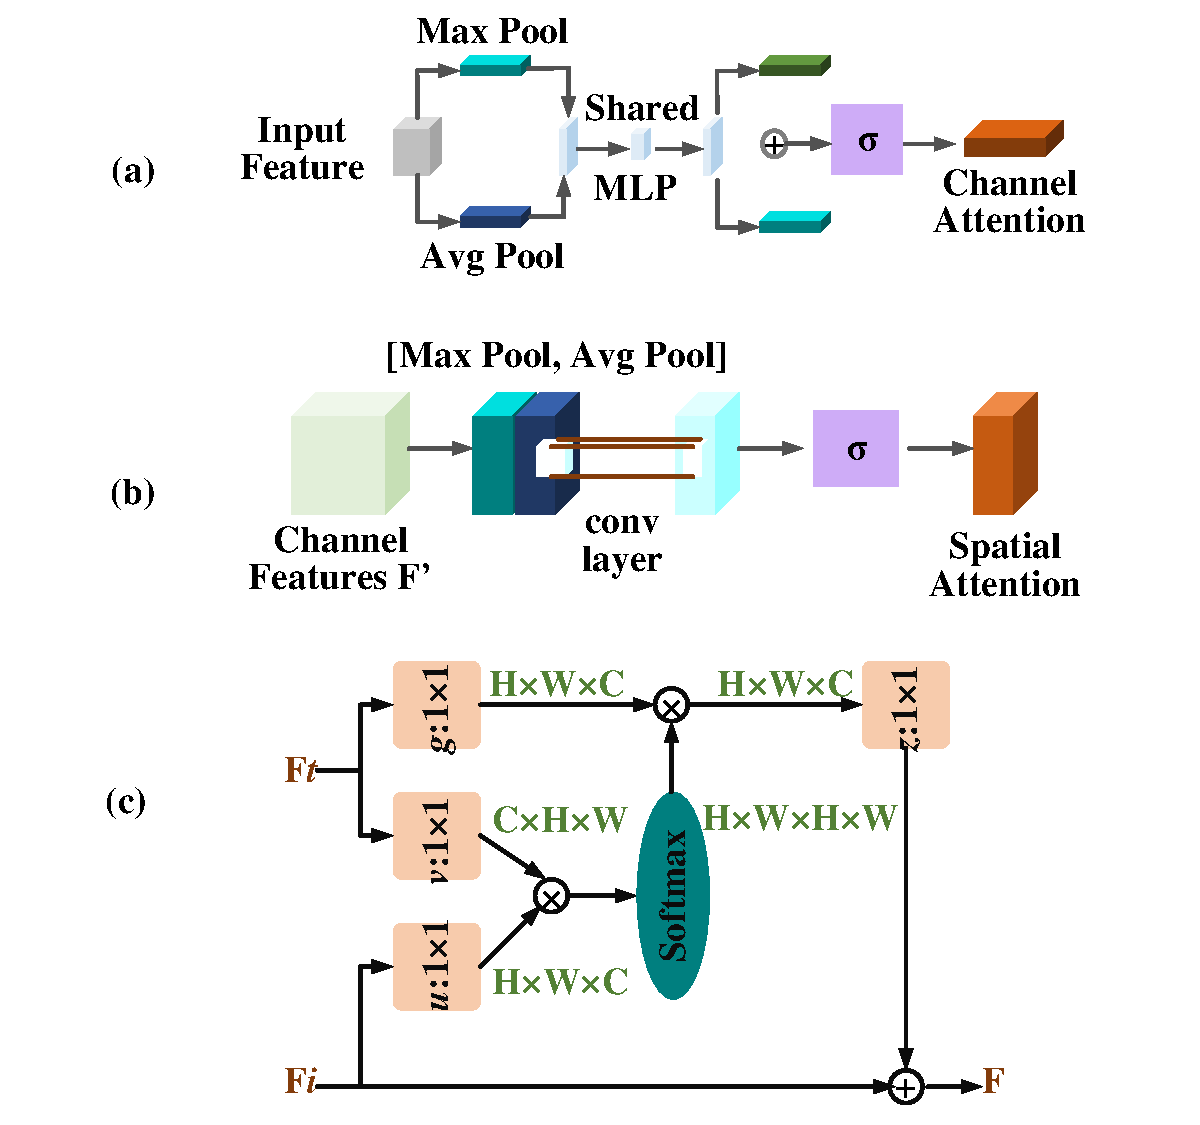
\includegraphics[width=\linewidth]{1FIGURE.pdf}}
    \caption {Different Attention mechanisms in image super-resolution (a) Channel Attention [19], (b) Spatial Attention [54], and (c) Non-Local Attention [49].}

    \label{fig1}

\end{figure}

The U-Net architecture, proposed by Ronneberger \textit{et al}. [4], was widely adopted in various image restoration tasks, including image super-resolution. In [4], an encoder-decoder architecture with skip connections facilitates low-level and high-level feature learning. The skip connections enable the network to combine low-level details with high-level semantic information, enhancing the reconstruction of fine image structures. U-Net [4] has been further improved by incorporating dilated convolutions, residual blocks, and other modifications to enhance its performance in SR tasks.
Inception blocks, introduced in GoogLeNet [60], have been widely utilized for multi-scale feature extraction in deep networks. Inception blocks consist of parallel convolutional layers with different receptive fields [61], allowing the model to capture information at multiple scales. This multi-scale representation learning enhances the network's ability to capture local and global structures, facilitating improved reconstruction quality. Inception blocks have been incorporated into SR models to capture diverse image features and enable more effective feature extraction.
While substantial progress has been made in the field of image super-resolution, there is still a need for techniques that can effectively capture long-range dependencies, exploit contextual information, and enhance the reconstruction of fine details. This work proposes a novel approach that combines non-local sparse attention with a U-Net network architecture augmented with inception blocks. Integrating these components aims to leverage the strengths of attention mechanisms, multi-scale feature extraction, and deep network architectures to enhance image super-resolution performance further.
In summary, deep learning-based approaches, attention mechanisms, and network architectures have significantly advanced in image super-resolution. Combining these techniques has led to significant improvements in reconstruction quality, enabling the generation of high-resolution images with enhanced details. Ongoing research addresses challenges such as computational efficiency, generalization across domains, and adapting SR techniques to video super-resolution [5]. These advancements are crucial for realizing the full potential of image super-resolution in various applications, including face image super-resolution [3], medical imaging [7], surveillance [6], remote sensing [11], and digital content creation [8, 62].


\begin{figure*}
    \centering

    \includegraphics[width=\linewidth]{2Figure.pdf}
    \caption{The proposed network architecture of Deep Attention Network for Single Image Super-Resolution (DANS).}
    \label{fig:2}
\end{figure*}

\section{PROPOSED METHOD}

This section presents our proposed novel approach in single image super-resolution by fusion of Non-Local Sparse attention mechanism [30] into U-Net [4] framework Network. Furthermore, we employed the inception block [60] in the network architecture to extract various contextual features at distinct levels of abstraction. Additionally, skip connections are introduced to transmit low-frequency information at each network stage to reduce the required parameters for the computation. The up-sampling and down-sampling are presented in the network to localize the high-resolution features to generate more precise results for the contextual regions in an image.

As shown in Figure 2, our proposed Deep Attention Network for Single Image Super-Resolution (DANS) comprises three staged encoder-decoder frameworks. Each stage consists of Inception Block and NLSA block. The architecture of DANS uses 5 NLSA [30] Blocks with up-sampling and down-sampling. It also contains six inception blocks to better understand fine-grained details and broader contextual details at different levels of abstraction. The image is enlarged by a factor of two at the encoder side and reduced by two at the decoder. The contextual details of an image are stored in high-frequency signals and are refined by propagating it through the encoder-decoder framework. In contrast, the low-frequency information is passed through the skip connections. This symmetric encoder-decoder design produces more precise SR results than a sequential model. Since hierarchical features [63] help to understand global and fine-grained details better, adopting an encoder-decoder framework by introducing up-sampling and down-sampling instead of adopting a sequential framework helps to learn hierarchical features in an image. It is to be noted that the encoder-decoder network is more flexible with variable input and output data [4]. The encoder can accommodate input of varying sizes, and the decoder can generate output with variable sizes. Also, encoder-decoder frameworks are well suited for structured outputs, i.e., processing images containing text. Therefore, each modality of images with text is processed independently by the encoder and integrated to generate joint representations of the output by the decoder. 

Instead of residual blocks, we have used inception blocks to extract features at various abstraction levels to capture global and local contextual details better. This is much more useful for object detection or scene understanding. Inception Block helps to achieve diverse and complementary sets of feature maps because of parallel pathways and different receptive fields [61]. The parameter sharing makes the inception block more compact than the residual block. The diversity of features captured benefits tasks requiring a wide range of visual patterns. 

The Deep Feature Extraction Block indicated by Body\_U and Body\_D in Figure 2 consists of two 3 $\times$ 3 convolutions, one Non-Local Sparse Attention Block and an up-sample module in Body\_U at the encoder side and down-sampler in Body\_D at the decoder side at each stage of the framework. Non-local sparse attention has shown brilliant performance in NLSN [30] for extracting contextual details in SISR, but it increases the computational cost when used in a sequential model. Our proposed approach uses NLSA block in an encoder-decoder framework to reduce the number of parameters and ultimately help reduce the computational cost compared to a sequential model framework. Since sparsity constraints in the NLSA block help focus on contextual details, the encoder-decoder framework preserves the spatial information in the model architecture. Therefore, using the NLSA block in this framework allows the decoder to easily access the preserved low-level features from the encoder through skip connections. 


\subsection{Deep Feature Extraction (DFE)}

Deep feature extraction is used to capture an image's textural and contextual features, also known as deep features. This technique mainly processes and refines the high-frequency information in the image patches. Deep Feature Extraction (DFE) is classified into two categories 1.) Deep Feature Extraction Up-Sampler Block, and 2.) Deep Feature Extraction Down-Sampler Block. As seen in Figure 2, at every stage, for the encoder side, we have used Deep Feature Extraction Up-Sampler Block termed Body\_U, and for the decoder, we have used Deep Feature Extraction Down-Sampler Block termed Body\_D.  

\subsubsection{ Deep Feature Extraction Up-Sampler}

As seen in Figure 3, the Deep Feature extraction Up-Sampler (DFE\_U) block consists of two 3 $\times$ 3 convolutional layers, one NLSA Block, and an up-sampling or down-sampling module stacked together. The 3 $\times$ 3 convolutional layers help to extract the local features to learn spatial and discriminative features [64] from the input data. The NLSA [30] blocks help to analyze the relationship between different spatial positions of the extracted features, and finally, the up-sampling module enlarges the derived characteristics. The output of the Deep Feature Extraction Up-Sampler Block is shown in Equation 1. 

\begin{equation}
{H_{0}}= {H_{DFE\_U}}({H_{IB}}),
\end{equation}
where ${H_{DFE\_U}}$$(.)$ represents deep feature extraction up-sampler operation, and $({H_{IB}})$ is the output of the inception block where the original input LR image is fed after passing through the depthwise separable convolution. After obtaining the up-sampled deep features, ${H_{0}}$ is used as the input of the next stage Inception block and the Deep Feature Extraction Down-Sampler Block DFE\_D.

\begin{figure}[ht]
  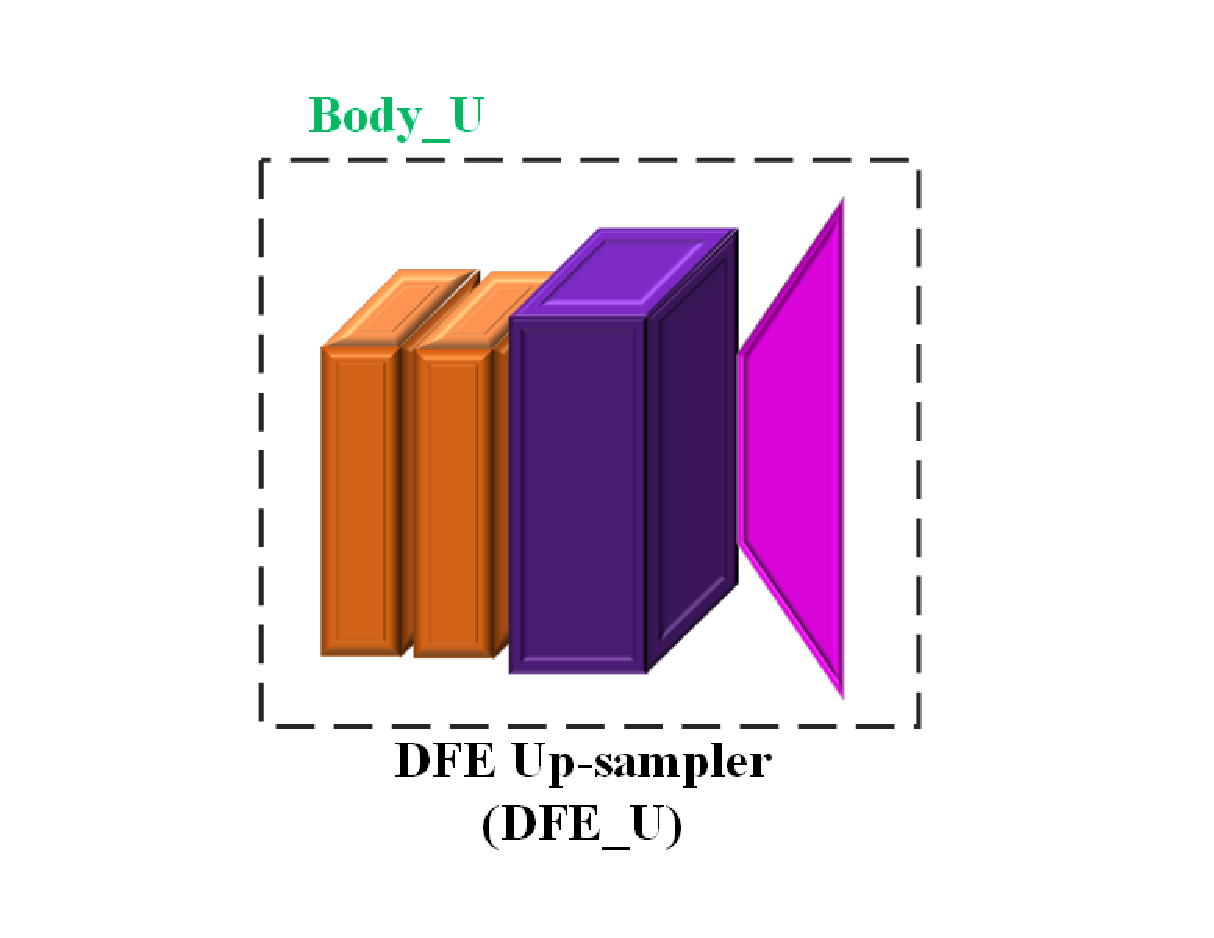
\includegraphics[width=\linewidth]{3FIGURE.pdf}
  \caption{The structure of Deep Feature Extraction Up-Sampler Block.}
  \label{fig:3}
\end{figure}

\subsubsection{Deep Feature Extraction Down-Sampler}

This block is described in Figure 4. It uses a down-sampling module to shrink the spatial resolution of the characteristic maps and aggregate details at a coarse scale. Like  DFE\_U, in Deep Feature extraction Down-Sampler (DFE\_D) also stack two 3$\times$3 convolutions with NLSA [30] block to capture deep contextual feature effectively. Still, instead of an up-sampler, we use a down-sampler to help downscale the extracted features to process through the NLSA [30] Block. The output of the Deep Feature Extraction Down-Sampler Block is shown in Equation 2. 
It is to be noted that the DFE\_D excepts two inputs, i.e., one from the DFE\_U Block and the other from the inception block.
\begin{equation}
{H_{I}}= {H_{DFE\_D}}({H_{IB}} + {H_{DFE\_U}}),
\end{equation}
where ${H_{DFE\_D}}$$(.)$ represents deep feature extraction down-sampling operation, and $({H_{IB}})$ is the output of the inception block. After obtaining the up-sampled deep features, ${H_{I}}$ is used as the input of the next stage Inception block and the Deep Feature Extraction Down-Sampler Block.

This process is repeated at each network stage, and the HR image is obtained after passing through the depth-wise separable convolution operation.

\begin{figure}[ht]
  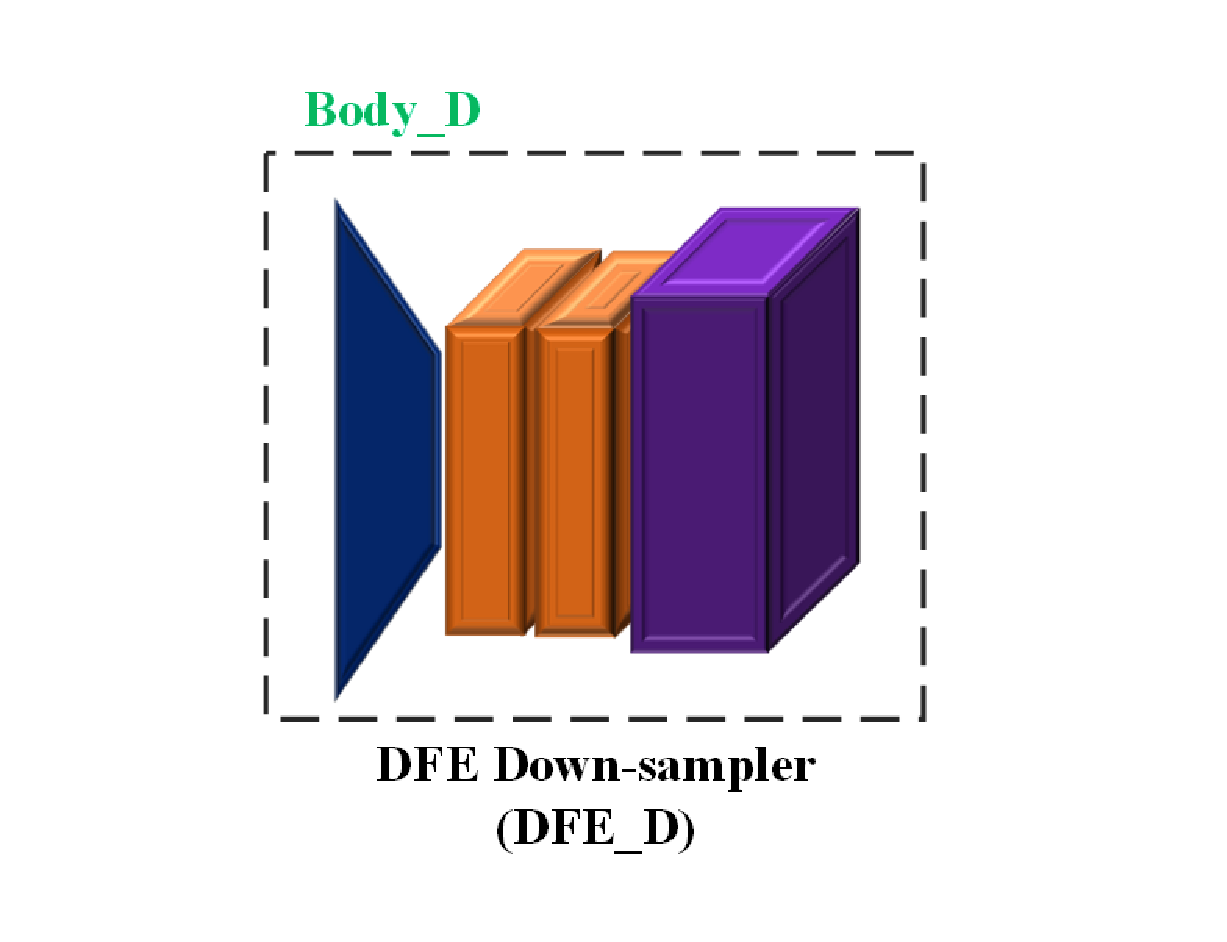
\includegraphics[width=\linewidth]{4FIGURE.pdf}
  \caption{The structure of Deep Feature Extraction Down-Sampler Block.}
  \label{fig:4}
\end{figure}

\subsection{Inception Block}
The Inception block, as seen in Figure 5, also known as the Inception module, is a building block of deep neural network architectures, originally introduced in the GoogLeNet [60] model for image classification. It is designed to capture information at multiple scales and learn diverse and rich feature representations.

The key idea behind the Inception block is to parallelize and concatenate multiple convolutional operations of different filter sizes, allowing the network to capture local and global information. This enables the model to learn a wide range of features at various levels of abstraction within the same layer.

The Inception block typically combines 1$\times$1, 3$\times$3, and 5$\times$5 convolutional filters, and max-pooling operations. It includes multiple parallel branches, each performing a different convolution operation. The final outputs of the Inception block are generated by concatenating these branches along the channel dimension. The 1$\times$1 convolutions are used to make the input less dimensional and control the computational complexity of the block.

One of the major advantages of the Inception block is its ability to efficiently capture regional and global details within a layer and maintain a minimum number of parameters while keeping a large receptive field [61]. This makes the Inception block effective for jobs such as image classification [65], object detection[1], and semantic segmentation [4].

In our proposed model, we used 1$\times$1 and 3$\times$3 convolutional layers inside the inception block followed by Rectified Linear Unit (ReLU) activation. We further controlled experiments by changing the activations to PReLU and CReLU to check their effect on the model's performance. 

\begin{figure}[ht]
  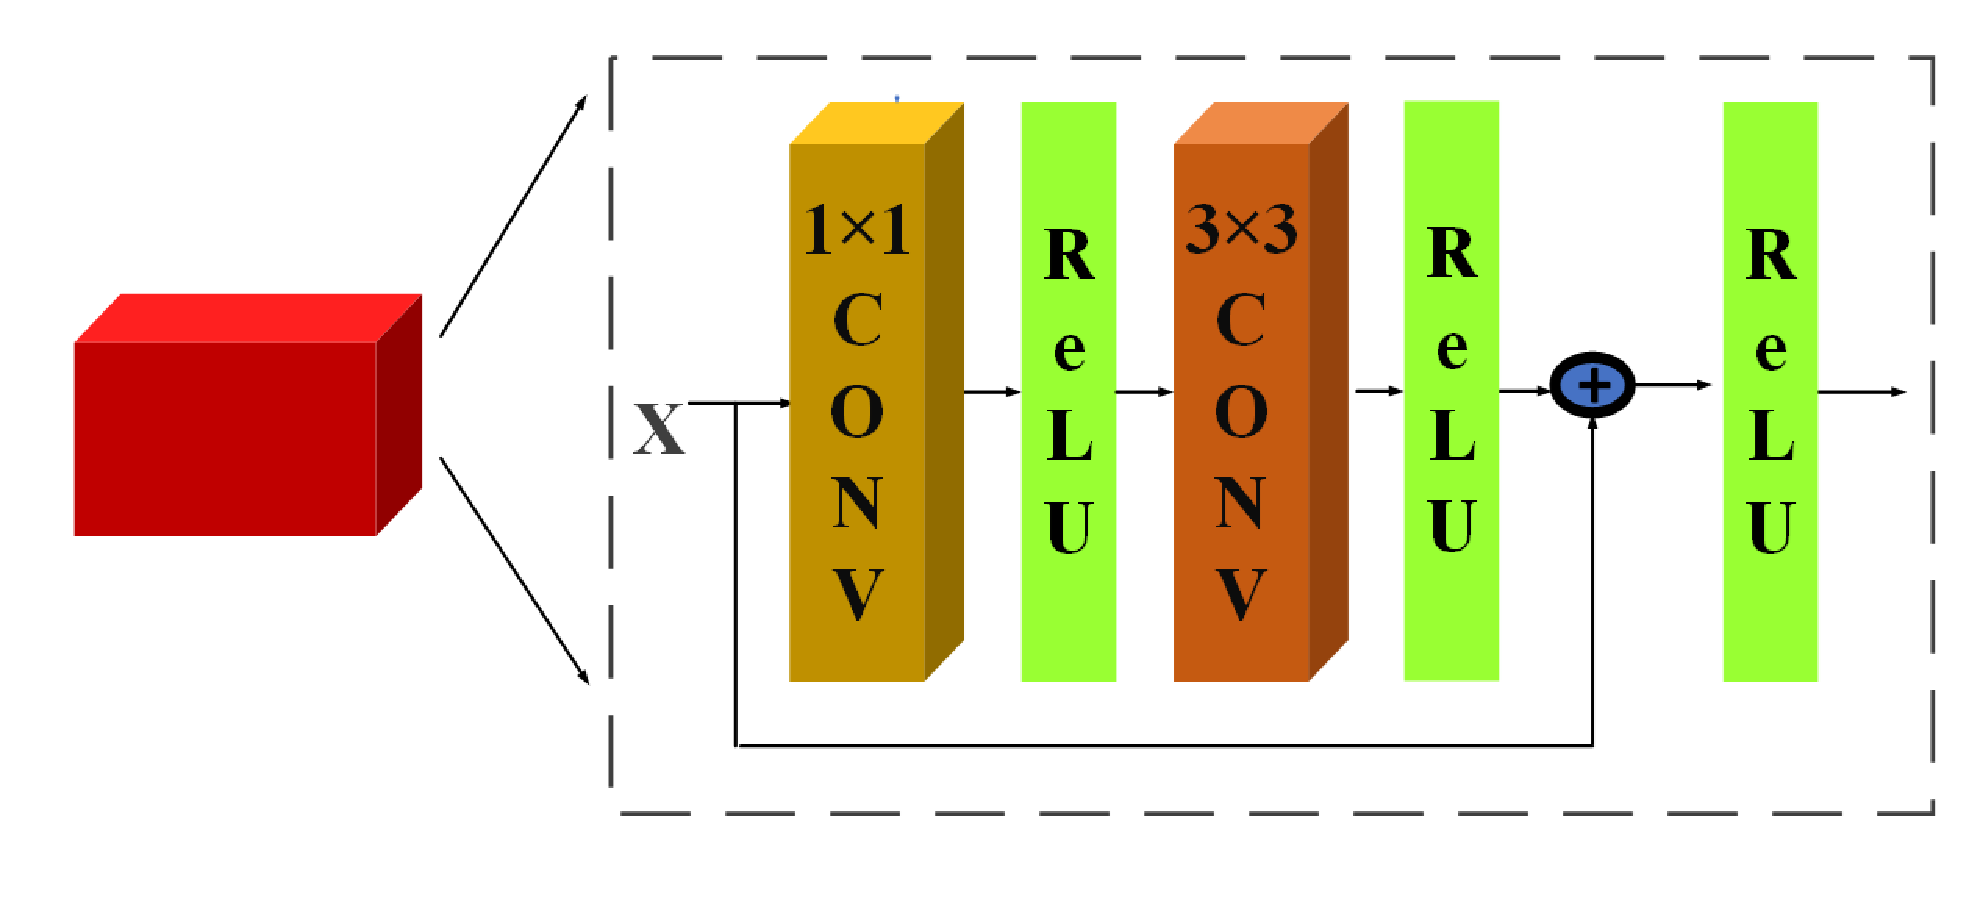
\includegraphics[width=\linewidth]{5FIGURE.pdf}
  \caption{ Inception Block }
  \label{fig:5}
\end{figure}

The potential applications of our proposed framework in image and computer vision tasks such as image segmentation, classification, and object detection. The main versatile application of our proposed approach is in medical imaging [7], image restoration [32], and video super-resolution [5], where efficient models are highly desirable. 

\section{Experimental Results}

To show the quantitative and qualitative visual results of our proposed DANS model, several experiments were conducted on benchmark test datasets to verify its performance. Furthermore, the computational cost in terms of network parameters and execution time are discussed in this section. Our model training performance is evaluated with average PSNR (dB)  and loss versus epoch convergence. Additionally, an ablation study has been shown for different rounds of NLSA [30] with the baseline during the testing process. Structural ablation study has been demonstrated by using different activation functions in the inception block and showing performance convergence per epoch. Finally, noise degradation analysis compared with different selective models has been presented to verify that our model also has better quantitative performance on noisy and blurry images.

\subsection{Experimental Settings} 
This section demonstrates the training details, evaluation metrics, and the datasets used in training and testing the effectiveness of our proposed model on public datasets. It is to be noted that the training and the testing sets are different. 

\subsubsection{Datasets} 

We used the DIV2K [66] dataset to train our SR model. It contains 800 high-quality training images. This dataset contains diversified variations in its images. For testing, we used five benchmark datasets for comparison, which are Set5 [67], Set14 [68], BSD100 [69], Manga109 [71], and Urban100 [70]. Table 1 shows the training and testing datasets with the number of images.

\begin{table}[htbp]
  \centering
  \caption{The total number of images available in the Training and Testing Dataset}
  \begin{tabular}{|c|c|c|c|} % Specify four columns with "c" for centered alignment
    \hline
    \textbf{Datasets} & \textbf{Train} & \textbf{Test} & \textbf{Number of Images} \\
    \hline
    DIV2K [66]   & \checkmark   & $\times$   & 800   \\
    Set5 [67]   & $\times$   & \checkmark   & 5   \\
    Set14 [68]   & $\times$   & \checkmark   & 14   \\
    BSD100 [69]   & $\times$   & \checkmark   & 100   \\
    Urban100 [70]   & $\times$   & \checkmark   & 100   \\    
    Manga109 [71]  & $\times$   & \checkmark   & 109   \\
% Add more rows as needed
    \hline
  \end{tabular}
\end{table}


\subsubsection{Training Details} 

We cropped random low-resolution patches with sizes 48 $\times$ 48 to train our model. The low-resolution images for $\times$2, $\times$3, $\times$4, and $\times$8 were obtained using MATLAB R2022b. The proposed network is trained on NVIDIA GeForce GTX 2080ti GPU with 24GB memory. Python 3.6 programming language with PyTorch 1.1.0 platform has been used for coding the algorithm of the proposed model. Eight hundred samples from DIV2K [66] datasets are obtained for training the model. We select an Adam optimizer with $\beta_1 = 0.90$ and $\beta_2 = 0.99$ for optimization purposes. The learning rate of the proposed model is kept being 10$^{-4}$ and reduced to half every 200 epochs. 

\subsubsection{Testing Details} 

Our proposed model has been tested on five standard benchmark datasets, i.e., Set5 [67], Set14 [68], BSD100 [69], Urban100 [70], and Manga109 [71] datasets. The LR image is obtained by downsampling the HR images using bicubic kernels. 48 $\times$ 48 patches are randomly cropped from the training samples and divided into mini-batches of 8 images. Data augmentation also creates more samples for the algorithm by flipping and randomly rotating for 90, 180, and 270 degrees. Input is expected to be 100 $\times$ 100 spatial with 64 input and output channels. The range of scaled images for LR is set in the range [- 1, 1]. The Mean Squared Error (MSE) has been computed on the image intensity range [-1, 1]. PSNR and SSIM are standard evaluation metrics for quantitatively comparing our model with state-of-the-art methods.


\subsection{Quantitative comparisons with state-of-the-art models}
Table 2 presents the tabular standard metric comparison of five benchmark test datasets. Quantitative analysis of our proposed DANS shows a comparison with seventeen SOTA methods, such as Bicubic, SRCNN [17], FSRCNN [72], VDSR [35], RDN [73], LapSRN [74], SENext [14], RCAN [19], MemNet [43], RNAN [75], MFCC [16], SRFBN [76], SAN [51], EDSR [22], HAN [50], SwinIR [77], and NLSN [30]. 
As shown in Table 2, our proposed DANS quantitative results have significantly outperformed the state-of-the-art methods in terms of PSNR and SSIM. Our proposed DANS model is better in performance on all test datasets for scale factors $\times2$, $\times3$, $\times4$, and $\times8$. Furthermore, our proposed method obtained a higher value of PSNR/SSIM on all averages compared to other SOTA models.


\begin{table*}
\caption{Quantitative evaluation of our proposed DANS with SR models. Average values of PSNR/SSIM have also been reported on enlargement factors $\times 2$, $\times 3$ $\times 4$, and $\times 8$. The best quantitative value has been recorded as bold with {\color{red}\textbf{Red }} color. The second-best quantitative value is shown in {\color{blue}\underline{blue}} color with an underline.}

\label{table2}
\setlength{\tabcolsep}{4.5 pt}
\begin{tabular}{|c|c|c|cc|cc|cc|cc|cc|cc|}
\hline
\multirow{2}{*}{Method} & \multirow{2}{*}{Factor} & \multirow{2}{*}{\#Param}& \multicolumn{2}{c|}{Set5 [67]}& \multicolumn{2}{c|}{Set14 [68]}& \multicolumn{2}{c|}{BSD100 [69]}& \multicolumn{2}{c|}{Urban100 [70]}& \multicolumn{2}{c|}{Manga109 [71]}& \multicolumn{2}{c|}{Average}\\


 \cline{4-15}&&& \multicolumn{1}{c|}{PSNR$\uparrow$}  & SSIM{$\uparrow$}   & \multicolumn{1}{c|}{PSNR$\uparrow$}  & SSIM {$\uparrow$}   & \multicolumn{1}{c|}{PSNR$\uparrow$}  & SSIM {$\uparrow$}   & \multicolumn{1}{c|}{PSNR$\uparrow$}  & SSIM {$\uparrow$}  & \multicolumn{1}{c|}{PSNR$\uparrow$}  & SSIM {$\uparrow$}   & \multicolumn{1}{c|}{PSNR$\uparrow$}  & SSIM {$\uparrow$}  \\
 \hline

Bicubic&$\times2$ & -/-& \multicolumn{1}{c|}{33.68 } & 0.9304  & \multicolumn{1}{c|}{30.24 } &0.8691  & \multicolumn{1}{c|}{29.56 } & 0.8435  & \multicolumn{1}{c|}{26.88 } & 0.8405  & \multicolumn{1}{c|}{31.05 } & 0.9349&
\multicolumn{1}{c|}{30.23} & 0.8832 \\


SRCNN [17] & $\times 2$ & 57K& \multicolumn{1}{c|}{36.66 } & 0.9542  & \multicolumn{1}{c|}{32.45 } & 0.9067  &\multicolumn{1}{c|}{31.36 } & 0.8879  & \multicolumn{1}{c|}{29.51 } &0.8946 & \multicolumn{1}{c|}{35.72} &0.9680
&\multicolumn{1}{c|}{33.11} & 0.9219\\

FSRCNN [72]& $\times 2$& 12K & \multicolumn{1}{c|}{36.98} &0.9556& \multicolumn{1}{c|}{32.62} & 0.9087 &\multicolumn{1}{c|}{31.50} &0.8904& \multicolumn{1}{c|}{29.58} &0.9009& \multicolumn{1}{c|}{36.62} &0.9710
&\multicolumn{1}{c|}{33.56} & 0.9260\\

VDSR [35]& $\times 2$&665K& \multicolumn{1}{c|}{37.53} & 0.9587 & \multicolumn{1}{c|}{33.05} & 0.9127 &\multicolumn{1}{c|}{31.90} & 0.8960& \multicolumn{1}{c|}{30.77} & 0.9141 & \multicolumn{1}{c|}{37.16} & 0.9740
&\multicolumn{1}{c|}{33.24} & 0.9314\\

MemNet [43] & $\times 2$&677K& \multicolumn{1}{c|}{37.78} & 0.9597  & \multicolumn{1}{c|}{33.28} &0.9142  &\multicolumn{1}{c|}{32.08} & 0.8978 & \multicolumn{1}{c|}{31.31} &0.9195  & \multicolumn{1}{c|}{37.72} &0.9740
&\multicolumn{1}{c|}{34.43} &0.9330\\

LapSRN [74] & $\times 2$&812K& \multicolumn{1}{c|}{37.52} & 0.9591 & \multicolumn{1}{c|}{32.99} & 0.9124 &\multicolumn{1}{c|}{31.80} & 0.8949 & \multicolumn{1}{c|}{30.41} &  0.9101 & \multicolumn{1}{c|}{37.53} &  0.9740
&\multicolumn{1}{c|}{33.87} & 0.9302\\

SENext [14] & $\times 2$ &97K& \multicolumn{1}{c|}{38.04} & {0.9608} & \multicolumn{1}{c|}{\color{blue}\underline{34.24}} &{ 0.9181} & \multicolumn{1}{c|}{32.21} & {0.8997}& \multicolumn{1}{c|}{32.43} &{0.9287}& \multicolumn{1}{c|}{38.79} &{0.9774} &\multicolumn{1}{c|}{35.14} & {0.9369}\\


RDN [73]& $\times 2$& 21,900K & \multicolumn{1}{c|}{38.24} &0.9614 & \multicolumn{1}{c|}{34.01} & 0.9212 &\multicolumn{1}{c|}{32.34} &0.9017& \multicolumn{1}{c|}{32.89} &0.9353& \multicolumn{1}{c|}{39.18} &0.9780
&\multicolumn{1}{c|}{35.33} & 0.9395\\

RCAN [19]& $\times 2$&16,000K& \multicolumn{1}{c|}{38.27} & 0.9614 & \multicolumn{1}{c|}{34.12} & 0.9216 &\multicolumn{1}{c|}{32.41} & 0.9027& \multicolumn{1}{c|}{33.34} & 0.9384 & \multicolumn{1}{c|}{39.44} & 0.9786
&\multicolumn{1}{c|}{35.52} & 0.9405\\

RNAN [75]& $\times 2$&1,350K& \multicolumn{1}{c|}{38.17} & 0.9611 & \multicolumn{1}{c|}{33.87} &0.9207 &\multicolumn{1}{c|}{32.32} & 0.9014& \multicolumn{1}{c|}{32.73} &0.9340 & \multicolumn{1}{c|}{39.23} & 0.9785
&\multicolumn{1}{c|}{35.26} & 0.9391\\

MFCC [16]& $\times 2$&1,861K& \multicolumn{1}{c|}{38.16} & 0.9606 & \multicolumn{1}{c|}{33.85} &0.9195 &\multicolumn{1}{c|}{32.28} & 0.9010& \multicolumn{1}{c|}{32.65} &0.9331 & \multicolumn{1}{c|}{39.11} & 0.9780
&\multicolumn{1}{c|}{35.21} & 0.9384\\

SRFBN [76]& $\times 2$&3,500K& \multicolumn{1}{c|}{38.11} &  0.9609  & \multicolumn{1}{c|}{33.82 } & 0.9196  &\multicolumn{1}{c|}{32.29} & 0.9010 & \multicolumn{1}{c|}{32.62} & 0.9328 & \multicolumn{1}{c|}{39.08} & 0.9779
&\multicolumn{1}{c|}{35.18} &0.9384\\

SAN [51]& $\times 2$&1,550K& \multicolumn{1}{c|}{38.31} &{\color{blue}\underline{0.9620}} & \multicolumn{1}{c|}{34.07} & 0.9213 &\multicolumn{1}{c|}{32.42} &0.9028& \multicolumn{1}{c|}{33.10} &0.9370 & \multicolumn{1}{c|}{39.32} & 0.9792
&\multicolumn{1}{c|}{35.44} &0.9404\\

EDSR [22] & $\times 2$&43,000K& \multicolumn{1}{c|}{38.11} & 0.9602 & \multicolumn{1}{c|}{33.92} & 0.9195  &\multicolumn{1}{c|}{32.32} & 0.9013 & \multicolumn{1}{c|}{32.93} & 0.9351  & \multicolumn{1}{c|}{39.10} & 0.9773
&\multicolumn{1}{c|}{35.28} &0.9386\\

HAN [50] & $\times 2$&3,230K& \multicolumn{1}{c|}{38.27} & 0.9614  & \multicolumn{1}{c|}{34.16} & 0.9217  &\multicolumn{1}{c|}{32.41} & 0.9027 & \multicolumn{1}{c|}{33.35} &0.9385& \multicolumn{1}{c|}{39.46} & 0.9785
&\multicolumn{1}{c|}{35.53} &0.9405\\

NLSN [30] & $\times 2$ &4,475K& \multicolumn{1}{c|}{38.34} & 0.9618 & \multicolumn{1}{c|}{34.08} & 0.9231 & \multicolumn{1}{c|}{32.43} & 0.9027 & \multicolumn{1}{c|}{33.42} &0.9394 & \multicolumn{1}{c|}{39.59} & 0.9789
&\multicolumn{1}{c|}{35.57} & 0.9412\\

SwinIR [77] & $\times 2$ &878K& \multicolumn{1}{c|}{\color{blue}\underline{38.38}} & {\color{blue}\underline{0.9620}} & \multicolumn{1}{c|}{\color{blue}\underline{34.24}} &{\color{blue}\underline{ 0.9233}} & \multicolumn{1}{c|}{\color{blue}\underline{32.47}} & {\color{blue}\underline{0.9032}} & \multicolumn{1}{c|}{\color{blue}\underline{33.51}} & {\color{blue}\underline{0.9401}} & \multicolumn{1}{c|}{\color{blue}\underline{39.70}} &{\color{blue}\underline{0.9794}}
&\multicolumn{1}{c|}{\color{blue}\underline{35.66}} & {\color{blue}\underline{ 0.9416}}\\

DANS (Ours) & $\times 2$ &2,456K& \multicolumn{1}{c|}{\color{red}\textbf{38.49}} &{\color{red}\textbf{0.9622}} & \multicolumn{1}{c|}{\color{red}\textbf{34.28} } &{\color{red}\textbf{ 0.9248}} & \multicolumn{1}{c|}{\color{red}\textbf{32.64}} &{\color{red}\textbf{0.9039}}& \multicolumn{1}{c|}{\color{red}\textbf{33.58}} &{\color{red}\textbf{0.9404}}& \multicolumn{1}{c|}{\color{red}\textbf{39.72}} &{\color{red}\textbf{0.9796}} &\multicolumn{1}{c|}{\color{red}\textbf{35.74}} & {\color{red}\textbf{0.9422}}\\
\hline

Bicubic&$\times3$ &-/-& \multicolumn{1}{c|}{30.40} & 0.8686  & \multicolumn{1}{c|}{27.54} & 0.7741 & \multicolumn{1}{c|}{27.21} & 0.7389 & \multicolumn{1}{c|}{24.46} & 0.7349  & \multicolumn{1}{c|}{26.95} &0.8566
&\multicolumn{1}{c|}{27.31} & 0.7945\\

SRCNN [17] & $\times3$ & 57K&\multicolumn{1}{c|}{32.75} & 0.9090  & \multicolumn{1}{c|}{29.29} & 0.8215  &\multicolumn{1}{c|}{28.41} & 0.7863  & \multicolumn{1}{c|}{26.24} &0.7991 & \multicolumn{1}{c|}{30.48} &0.9117
&\multicolumn{1}{c|}{29.44} & 0.8455\\

FSRCNN [72]& $\times3$ &12K& \multicolumn{1}{c|}{33.16} &0.9140& \multicolumn{1}{c|}{29.42} & 0.8242 &\multicolumn{1}{c|}{28.52} & 0.7893& \multicolumn{1}{c|}{26.41} &0.8064& \multicolumn{1}{c|}{31.10} &0.9210
&\multicolumn{1}{c|}{29.70} & 0.8516\\

VDSR [35]& $\times3$ &665K& \multicolumn{1}{c|}{33.66} & 0.9213 & \multicolumn{1}{c|}{29.78} & 0.8318 &\multicolumn{1}{c|}{28.83} & 0.7976& \multicolumn{1}{c|}{27.14} & 0.8279 & \multicolumn{1}{c|}{32.01} & 0.9340
&\multicolumn{1}{c|}{30.28} & 0.8624\\

MemNet [43] & $\times3$ &677K& \multicolumn{1}{c|}{34.09} &0.9248  & \multicolumn{1}{c|}{30.00} &0.8350  &\multicolumn{1}{c|}{28.96} & 0.8001 & \multicolumn{1}{c|}{27.56} & 0.8376 & \multicolumn{1}{c|}{32.51} &0.9369
&\multicolumn{1}{c|}{ 30.62} &0.8669\\

LapSRN [74] &$\times3$ &812K& \multicolumn{1}{c|}{33.82} & 0.9227  & \multicolumn{1}{c|}{29.79} & 0.8320  &\multicolumn{1}{c|}{28.82} & 0.7973  & \multicolumn{1}{c|}{27.07} & 0.8271 & \multicolumn{1}{c|}{32.21} & 0.9350
&\multicolumn{1}{c|}{30.36} & 0.8631\\

SENext [14] & $\times3$ &54K& \multicolumn{1}{c|}{34.32} &{0.9255}& \multicolumn{1}{c|}{\color{red}\textbf{31.08}} & {0.8419} & \multicolumn{1}{c|}{29.11} &{0.8047}& \multicolumn{1}{c|}{28.60} &{0.8519}& \multicolumn{1}{c|}{33.63} &{0.9451} &\multicolumn{1}{c|}{31.35} &{0.8738} \\

RDN [73]& $\times3$ &21,900K& \multicolumn{1}{c|}{34.71} &0.9296& \multicolumn{1}{c|}{30.57} & 0.8468 &\multicolumn{1}{c|}{29.26} & 0.8093& \multicolumn{1}{c|}{28.80} &0.8653& \multicolumn{1}{c|}{34.13} &0.9484
&\multicolumn{1}{c|}{31.49} & 0.8798\\

RCAN [19]& $\times3$ &16,000K& \multicolumn{1}{c|}{34.74} & 0.9299 & \multicolumn{1}{c|}{30.65} & 0.8482 &\multicolumn{1}{c|}{29.32} & 0.8111& \multicolumn{1}{c|}{29.09} & 0.8702 & \multicolumn{1}{c|}{34.44} & 0.9499
&\multicolumn{1}{c|}{31.64} & 0.8818\\

RNAN [75]& $\times3$ &1,350K& \multicolumn{1}{c|}{34.66} & 0.9290 & \multicolumn{1}{c|}{30.52} & 0.8462 &\multicolumn{1}{c|}{29.32} & 0.8090& \multicolumn{1}{c|}{28.75} & 0.8646 & \multicolumn{1}{c|}{34.25} & 0.9483
&\multicolumn{1}{c|}{31.50} & 0.8794\\

MFCC [16]& $\times 3$&2,230K& \multicolumn{1}{c|}{34.67} & 0.9294 & \multicolumn{1}{c|}{30.51} &0.8456 &\multicolumn{1}{c|}{29.22} & 0.8080& \multicolumn{1}{c|}{28.64} & 0.8616 & \multicolumn{1}{c|}{34.15} & 0.9478
&\multicolumn{1}{c|}{31.43} & 0.8793\\

SRFBN [76]&$\times3$ &3,500K& \multicolumn{1}{c|}{34.70} & 0.9292 & \multicolumn{1}{c|}{30.51} &0.8461 &\multicolumn{1}{c|}{29.24} & 0.8084& \multicolumn{1}{c|}{28.73} & 0.8641 & \multicolumn{1}{c|}{34.18} & 0.9481
&\multicolumn{1}{c|}{31.47} & 0.8791\\

SAN [51]& $\times3$ &1,550K& \multicolumn{1}{c|}{34.75} &  0.9300 & \multicolumn{1}{c|}{30.59} & 0.8476 &\multicolumn{1}{c|}{29.33} & 0.8112 & \multicolumn{1}{c|}{28.93} & 0.8671 & \multicolumn{1}{c|}{34.30} & 0.9494
&\multicolumn{1}{c|}{31.58} &  0.8810\\

EDSR [22]& $\times3$&43,000K& \multicolumn{1}{c|}{34.65} & 0.9280 & \multicolumn{1}{c|}{30.52} & 0.8462 &\multicolumn{1}{c|}{29.25} & 0.8093& \multicolumn{1}{c|}{28.80} & 0.8653 & \multicolumn{1}{c|}{34.17} & 0.9476
&\multicolumn{1}{c|}{31.48} &0.8792\\

HAN [50] & $\times3$&3,230K& \multicolumn{1}{c|}{34.75} & 0.9299 & \multicolumn{1}{c|}{30.67} & 0.8483 &\multicolumn{1}{c|}{29.32} & 0.8110 & \multicolumn{1}{c|}{29.10} & 0.8705 & \multicolumn{1}{c|}{34.48} & 0.9500
&\multicolumn{1}{c|}{31.66} &0.8819\\

NLSN [30] & $\times3$ &4,475K& \multicolumn{1}{c|}{34.85} & 0.9306& \multicolumn{1}{c|}{30.70} &0.8485 &\multicolumn{1}{c|}{29.34} & 0.8117& \multicolumn{1}{c|}{29.25} & 0.8726& \multicolumn{1}{c|}{34.57} & 0.9508
&\multicolumn{1}{c|}{31.74} &0.8824\\

SwimIR [77] & $\times3$ &886K& \multicolumn{1}{c|}{\color{blue}\underline{34.89}} & {\color{blue}\underline{0.9312}} & \multicolumn{1}{c|}{30.77} &{\color{blue}\underline{0.8503}} & \multicolumn{1}{c|}{\color{blue}\underline{29.37}} & {\color{blue}\underline{0.8124}} & {\color{blue}\underline{29.29}} & {\color{blue}\underline{0.8744}}& \multicolumn{1}{c|}{\color{blue}\underline{34.74}} &{\color{blue}\underline{0.9518}} &\multicolumn{1}{c|}{\color{blue}\underline{31.81}} & {\color{blue}\underline{0.8840}}\\

DANS (Ours) & $\times3$ &2,456K& \multicolumn{1}{c|}{\color{red}\textbf{34.96}} &{\color{red}\textbf{0.9329}}& \multicolumn{1}{c|}{\color{blue}\underline{30.88}} & {\color{red}\textbf{0.8512}}& \multicolumn{1}{c|}{\color{red}\textbf{29.42}} &{\color{red}\textbf{0.8132}}& \multicolumn{1}{c|}{\color{red}\textbf{29.31}} &{\color{red}\textbf{0.8752}}& \multicolumn{1}{c|}{\color{red}\textbf{34.88}} &{\color{red}\textbf{0.9519}} &\multicolumn{1}{c|}{\color{red}\textbf{31.89}} &{\color{red}\textbf{0.8848}}\\

\hline

Bicubic&$\times4$ &-/-& \multicolumn{1}{c|}{28.43 } &0.8109 & \multicolumn{1}{c|}{26.00  } &0.7023& \multicolumn{1}{c|}{25.96 } & 0.6678  & \multicolumn{1}{c|}{23.14 } & 0.6574  & \multicolumn{1}{c|}{25.15} &0.7890

&\multicolumn{1}{c|}{25.68} &0.7250\\


SRCNN [17] & $\times4$  &57K& \multicolumn{1}{c|}{30.48 } &0.8628   & \multicolumn{1}{c|}{27.50 } &0.7513  &\multicolumn{1}{c|}{ 26.90 } & 0.7103 & \multicolumn{1}{c|}{24.52 } &0.7226 & \multicolumn{1}{c|}{27.66 } &0.8580
&\multicolumn{1}{c|}{ 27.40} &0.7785 \\

FSRCNN [72]& $\times4$ &12K& \multicolumn{1}{c|}{30.70} & 0.8657& \multicolumn{1}{c|}{27.59} &0.7535  &\multicolumn{1}{c|}{26.96} &0.7128 & \multicolumn{1}{c|}{24.60} &0.7258 & \multicolumn{1}{c|}{27.89 } &0.8590
&\multicolumn{1}{c|}{27.57} &0.7850 \\

VDSR [35]& $\times4$ &665K & \multicolumn{1}{c|}{31.35} &0.8838 & \multicolumn{1}{c|}{28.02} & 0.7678&\multicolumn{1}{c|}{27.29} &0.7252 & \multicolumn{1}{c|}{25.18} &0.7525 & \multicolumn{1}{c|}{28.82 } & 0.8860
&\multicolumn{1}{c|}{28.13} &0.8031 \\

MemNet [43] & $\times4$ &677K& \multicolumn{1}{c|}{31.74} &0.8893& \multicolumn{1}{c|}{28.26} &0.7723 &\multicolumn{1}{c|}{27.40} &0.7281& \multicolumn{1}{c|}{25.50} &0.7630& \multicolumn{1}{c|}{29.42} & 0.8942
&\multicolumn{1}{c|}{28.46} &0.8094\\

LapSRN [74] & $\times4$ &812K& \multicolumn{1}{c|}{31.54} &0.8866 & \multicolumn{1}{c|}{28.09} &0.7694  &\multicolumn{1}{c|}{27.32} &0.7264  & \multicolumn{1}{c|}{25.21 } &0.7553   & \multicolumn{1}{c|}{29.09 } &0.8900
&\multicolumn{1}{c|}{28.27 } &0.8060 \\

SENext [14] & $\times4$  &54K& \multicolumn{1}{c|}{31.50} &0.8947  & \multicolumn{1}{c|}{\color{red}\textbf{28.99}} &{0.7812}  & \multicolumn{1}{c|}{\color{red}\textbf{28.49}} &{0.7357} & \multicolumn{1}{c|}{26.64 } &{0.7839}  & \multicolumn{1}{c|}{30.48} &{0.9084}
&\multicolumn{1}{c|}{29.22} &{0.8208}    \\

RDN [73]& $\times4$ &21,900K& \multicolumn{1}{c|}{32.47} & 0.8990& \multicolumn{1}{c|}{28.81} &0.7871  &\multicolumn{1}{c|}{27.72} &0.7419 & \multicolumn{1}{c|}{26.61} &0.8028 & \multicolumn{1}{c|}{31.00 } &0.9151
&\multicolumn{1}{c|}{29.32} &0.8291 \\

RCAN [19]& $\times4$ &16,000K & \multicolumn{1}{c|}{32.63} &0.9002 & \multicolumn{1}{c|}{28.87} & 0.7889&\multicolumn{1}{c|}{27.77} &0.7436 & \multicolumn{1}{c|}{26.82} &0.8087 & \multicolumn{1}{c|}{31.22 } & 0.9173
&\multicolumn{1}{c|}{29.46} &0.8317 \\

RNAN [75]& $\times4$ &1,350K& \multicolumn{1}{c|}{32.49} &0.8982  & \multicolumn{1}{c|}{28.83 } &0.7878 &\multicolumn{1}{c|}{27.72} &0.7421 & \multicolumn{1}{c|}{26.61 } &0.8023 & \multicolumn{1}{c|}{31.09 } & 0.9149
&\multicolumn{1}{c|}{29.34 } &0.8291 \\

MFCC [16]& $\times 4$&2,157K& \multicolumn{1}{c|}{32.42} & 0.8973 & \multicolumn{1}{c|}{28.73} &0.7849 &\multicolumn{1}{c|}{27.67} & 0.7399 & \multicolumn{1}{c|}{26.48} &0.7977 & \multicolumn{1}{c|}{30.98} & 0.9131
&\multicolumn{1}{c|}{29.25} & 0.8265\\

SRFBN [76]& $\times4$ &3,500K& \multicolumn{1}{c|}{32.47} &0.8983 & \multicolumn{1}{c|}{28.81} &0.7868 &\multicolumn{1}{c|}{27.72} &0.7409 & \multicolumn{1}{c|}{26.60} &0.8015 & \multicolumn{1}{c|}{31.15} & 0.9160
&\multicolumn{1}{c|}{29.35} &0.8287  \\

SAN [51]& $\times4$ &1,550K& \multicolumn{1}{c|}{32.64} &0.9003 & \multicolumn{1}{c|}{28.92} & 0.7888 &\multicolumn{1}{c|}{27.78} &0.7436 & \multicolumn{1}{c|}{26.79} &0.8068 & \multicolumn{1}{c|}{31.18} & 0.9169
&\multicolumn{1}{c|}{29.46} &0.8312 \\

EDSR [22] & $\times4$ &43,000K& \multicolumn{1}{c|}{32.46} &0.8968& \multicolumn{1}{c|}{28.80} &0.7876 &\multicolumn{1}{c|}{27.71} &0.7420 & \multicolumn{1}{c|}{26.64 } & 0.8033 & \multicolumn{1}{c|}{31.02} & 0.9148
&\multicolumn{1}{c|}{29.32} &0.8289  \\

HAN [50] & $\times4$ &3,230K& \multicolumn{1}{c|}{32.64 } &0.9002 & \multicolumn{1}{c|}{28.90} &0.7890 &\multicolumn{1}{c|}{27.80} &0.7442& \multicolumn{1}{c|}{26.85} &0.8094 & \multicolumn{1}{c|}{31.42} &0.9177
&\multicolumn{1}{c|}{29.52} &0.8321 \\

NLSN [30] & $\times4$ &4,475K& \multicolumn{1}{c|}{32.59 } &0.9000 & \multicolumn{1}{c|}{28.87} &0.7891 &\multicolumn{1}{c|}{27.78} &0.7444 & \multicolumn{1}{c|}{26.96} &0.8109 & \multicolumn{1}{c|}{31.27} &0.9184
&\multicolumn{1}{c|}{29.49} &0.8325 \\

SwinIR [77] & $\times4$  &897K& \multicolumn{1}{c|}{\color{blue}\underline{32.72}} &{\color{blue}\underline{0.9021}} & \multicolumn{1}{c|}{28.94} &{\color{blue}\underline{0.7914}}& \multicolumn{1}{c|}{27.83} &{\color{blue}\underline{0.7459}} & \multicolumn{1}{c|}{\color{blue}\underline{27.07}} &{\color{blue}\underline{0.8164}}& \multicolumn{1}{c|}{\color{blue}\underline{31.67}} &{\color{blue}\underline{0.9226}} &\multicolumn{1}{c|}{\color{blue}\underline{29.64}} &{\color{blue}\underline{0.8356}}  \\

DANS (Ours) & $\times4$  &2,456K& \multicolumn{1}{c|}{\color{red}\textbf{32.78}} &{\color{red}\textbf{0.9028}}  & \multicolumn{1}{c|}{\color{blue}\underline{28.98}} &{\color{red}\textbf{0.7928}}  & \multicolumn{1}{c|}{\color{blue}\underline{27.97}} &{\color{red}\textbf{0.7468}} & \multicolumn{1}{c|}{\color{red}\textbf{27.32 }} &{\color{red}\textbf{0.8189}}  & \multicolumn{1}{c|}{\color{red}\textbf{31.74}} &{\color{red}\textbf{0.9228}} &\multicolumn{1}{c|}{\color{red}\textbf{29.75}} &{\color{red}\textbf{0.8368}}    \\
\hline

Bicubic&$\times8$ &-/-& \multicolumn{1}{c|}{24.40} &0.6580& \multicolumn{1}{c|}{23.10} &0.5660 & \multicolumn{1}{c|}{23.67} &0.5480& \multicolumn{1}{c|}{20.74} &0.5160 & \multicolumn{1}{c|}{21.47} & 0.6500
&\multicolumn{1}{c|}{22.68} & 0.5876     \\

SRCNN [17] & $\times8$ &57K& \multicolumn{1}{c|}{25.33} & 0.6900 & \multicolumn{1}{c|}{23.76} &0.5910 &\multicolumn{1}{c|}{24.13} &0.5660 & \multicolumn{1}{c|}{21.29} &0.5440& \multicolumn{1}{c|}{22.46} &0.6950
&\multicolumn{1}{c|}{23.42} & 0.5739      \\

FSRCNN [72]& $\times8$&12K& \multicolumn{1}{c|}{25.60} &0.6970 & \multicolumn{1}{c|}{24.00} &0.5990&\multicolumn{1}{c|}{24.31} &0.5720 & \multicolumn{1}{c|}{21.45} &0.5500 & \multicolumn{1}{c|}{22.72} & 0.6920
&\multicolumn{1}{c|}{23.46} &  0.5696      \\

VDSR [35]& $\times8$&665K& \multicolumn{1}{c|}{25.93} &0.7240& \multicolumn{1}{c|}{24.26} &0.6140 &\multicolumn{1}{c|}{24.49} &0.5830 & \multicolumn{1}{c|}{21.70} &0.5710 & \multicolumn{1}{c|}{23.16} &0.7250
&\multicolumn{1}{c|}{23.50} & 0.5800       \\

MemNet [43]& $\times8$&677K& \multicolumn{1}{c|}{26.16} &  0.7414 & \multicolumn{1}{c|}{24.38} & 0.6199&\multicolumn{1}{c|}{24.58} & 0.5842 & \multicolumn{1}{c|}{21.89  } &0.5825 & \multicolumn{1}{c|}{23.56 } &0.7387
&\multicolumn{1}{c|}{24.11  } &  0.6529       \\

LapSRN [74]& $\times8$&812K& \multicolumn{1}{c|}{26.15} &0.7380& \multicolumn{1}{c|}{24.35} &0.6200 &\multicolumn{1}{c|}{24.54} &0.5860 & \multicolumn{1}{c|}{21.81} &0.5810 & \multicolumn{1}{c|}{23.39} &0.7350
&\multicolumn{1}{c|}{24.04} & 0.6520       \\

MSRN [44]& $\times8$&6,226K& \multicolumn{1}{c|}{26.59} &  0.7254 & \multicolumn{1}{c|}{24.88} & 0.5961&\multicolumn{1}{c|}{24.70} & 0.5610 & \multicolumn{1}{c|}{22.37 } & 0.6077 & \multicolumn{1}{c|}{24.30 } &0.7701
&\multicolumn{1}{c|}{24.56  } &  0.6520       \\

SENext [14] & $\times8$ &97K& \multicolumn{1}{c|}{26.87} &{0.7415} & \multicolumn{1}{c|}{\color{red}\textbf{25.73}} &{0.6200} & \multicolumn{1}{c|}{\color{red}\textbf{26.79}} &{0.5847} & \multicolumn{1}{c|}{21.90} &{0.5829} & \multicolumn{1}{c|}{23.96} &{0.7389} &\multicolumn{1}{c|}{25.05} &{0.6536}  \\


EDSR [22]& $\times8$&43,000K& \multicolumn{1}{c|}{26.96} &  0.7762 & \multicolumn{1}{c|}{24.91} & 0.6420&\multicolumn{1}{c|}{24.81} & 0.5985 & \multicolumn{1}{c|}{22.51  } &0.6221 & \multicolumn{1}{c|}{24.69 } &0.7841
&\multicolumn{1}{c|}{24.74  } &  0.6824       \\

AWSRN [78]& $\times8$&2,348K& \multicolumn{1}{c|}{26.97} &  0.7747 & \multicolumn{1}{c|}{24.96} & 0.6414&\multicolumn{1}{c|}{24.80} & 0.5967 & \multicolumn{1}{c|}{22.45  } &0.6174 & \multicolumn{1}{c|}{24.69 } &0.7842
&\multicolumn{1}{c|}{24.77  } &  0.6828       \\

DBPN [2]& $\times8$&10,000K& \multicolumn{1}{c|}{26.96} &  0.7762 & \multicolumn{1}{c|}{24.91} & 0.6420&\multicolumn{1}{c|}{24.81} & 0.5985 & \multicolumn{1}{c|}{22.51  } &0.6221 & \multicolumn{1}{c|}{24.60 } &0.7732
&\multicolumn{1}{c|}{24.75  } &  0.6824       \\

MFCC [16]& $\times8$&2,453K& \multicolumn{1}{c|}{27.07} &  0.7762 & \multicolumn{1}{c|}{25.01} & 0.6412&\multicolumn{1}{c|}{24.84} & 0.5980 & \multicolumn{1}{c|}{22.54  } &0.6196 & \multicolumn{1}{c|}{24.63 } &0.7791
&\multicolumn{1}{c|}{24.81  } &  0.6828       \\


RDN [73]& $\times8$&21,900K& \multicolumn{1}{c|}{27.21} &  0.7840 & \multicolumn{1}{c|}{25.13} & 0.6480&\multicolumn{1}{c|}{24.88} & 0.6010 & \multicolumn{1}{c|}{22.73  } &0.6312 & \multicolumn{1}{c|}{25.14 } &0.7897
&\multicolumn{1}{c|}{25.02  } &  0.6907       \\

RCAN [19]& $\times8$&16,000K& \multicolumn{1}{c|}{27.31} &  0.7878 & \multicolumn{1}{c|}{25.23} & {\color{blue}\underline{0.6511}}&\multicolumn{1}{c|}{24.98} & 0.6058 & \multicolumn{1}{c|}{\color{blue}\underline{23.00}} &{\color{blue}\underline{0.6452}} & \multicolumn{1}{c|}{\color{blue}\underline{25.24 }} &{\color{blue}\underline{0.8029}}
&\multicolumn{1}{c|}{\color{blue}\underline{25.15}} &  {\color{blue}\underline{0.6985}}       \\

HAN [50] & $\times8$&3,230K& \multicolumn{1}{c|}{\color{blue}\underline{27.33}} &{\color{blue}\underline{0.7884}}   & \multicolumn{1}{c|}{25.24} & 0.6510   &\multicolumn{1}{c|}{24.98} &{\color{blue}\underline{0.6059}}   & \multicolumn{1}{c|}{22.98} &{0.6437} & \multicolumn{1}{c|}{25.20}  &{0.8011} &\multicolumn{1}{c|}{25.14} &{0.6980} \\

DANS (Ours) & $\times8$ &2,456K& \multicolumn{1}{c|}{\color{red}\textbf{27.58}} &{\color{red}\textbf{0.7908}} & \multicolumn{1}{c|}{\color{blue}\underline{25.32}} &{\color{red}\textbf{0.6516}} & \multicolumn{1}{c|}{\color{blue}\underline{25.12}} &{\color{red}\textbf{0.6066}} & \multicolumn{1}{c|}{\color{red}\textbf{23.18}} &{\color{red}\textbf{0.6458}} & \multicolumn{1}{c|}{\color{red}\textbf{25.38}} &{\color{red}\textbf{0.8036}} &\multicolumn{1}{c|}{\color{red}\textbf{25.31}} &{\color{red}\textbf{0.6996}}  \\

\hline


\end{tabular}
\end{table*}



\subsection{Comparison analysis based on the number of model parameters}
In Figure 6, the comparison in parameters versus PSNR has been shown for our proposed DANS model. The performance is evaluated on the Set5 [67] test dataset for our proposed model DANS with an enlargement factor of $\times 2$. A reduction in the number of parameters demonstrates a reduction in computational cost. Compared to other deep learning models, the DANS model helps reduce the model's size better. DANS has parameters about 94\% less than EDSR [22], 84\% less than RCAN [19], 88\% less than RDN [73], 45\% less than NLSN [30], 23\% less than HAN [50], and 29\% less than SRFBN [76]. Figure 6 shows that our proposed method has lesser parameters than six other state-of-the-art methods.

\begin{figure}[ht]
  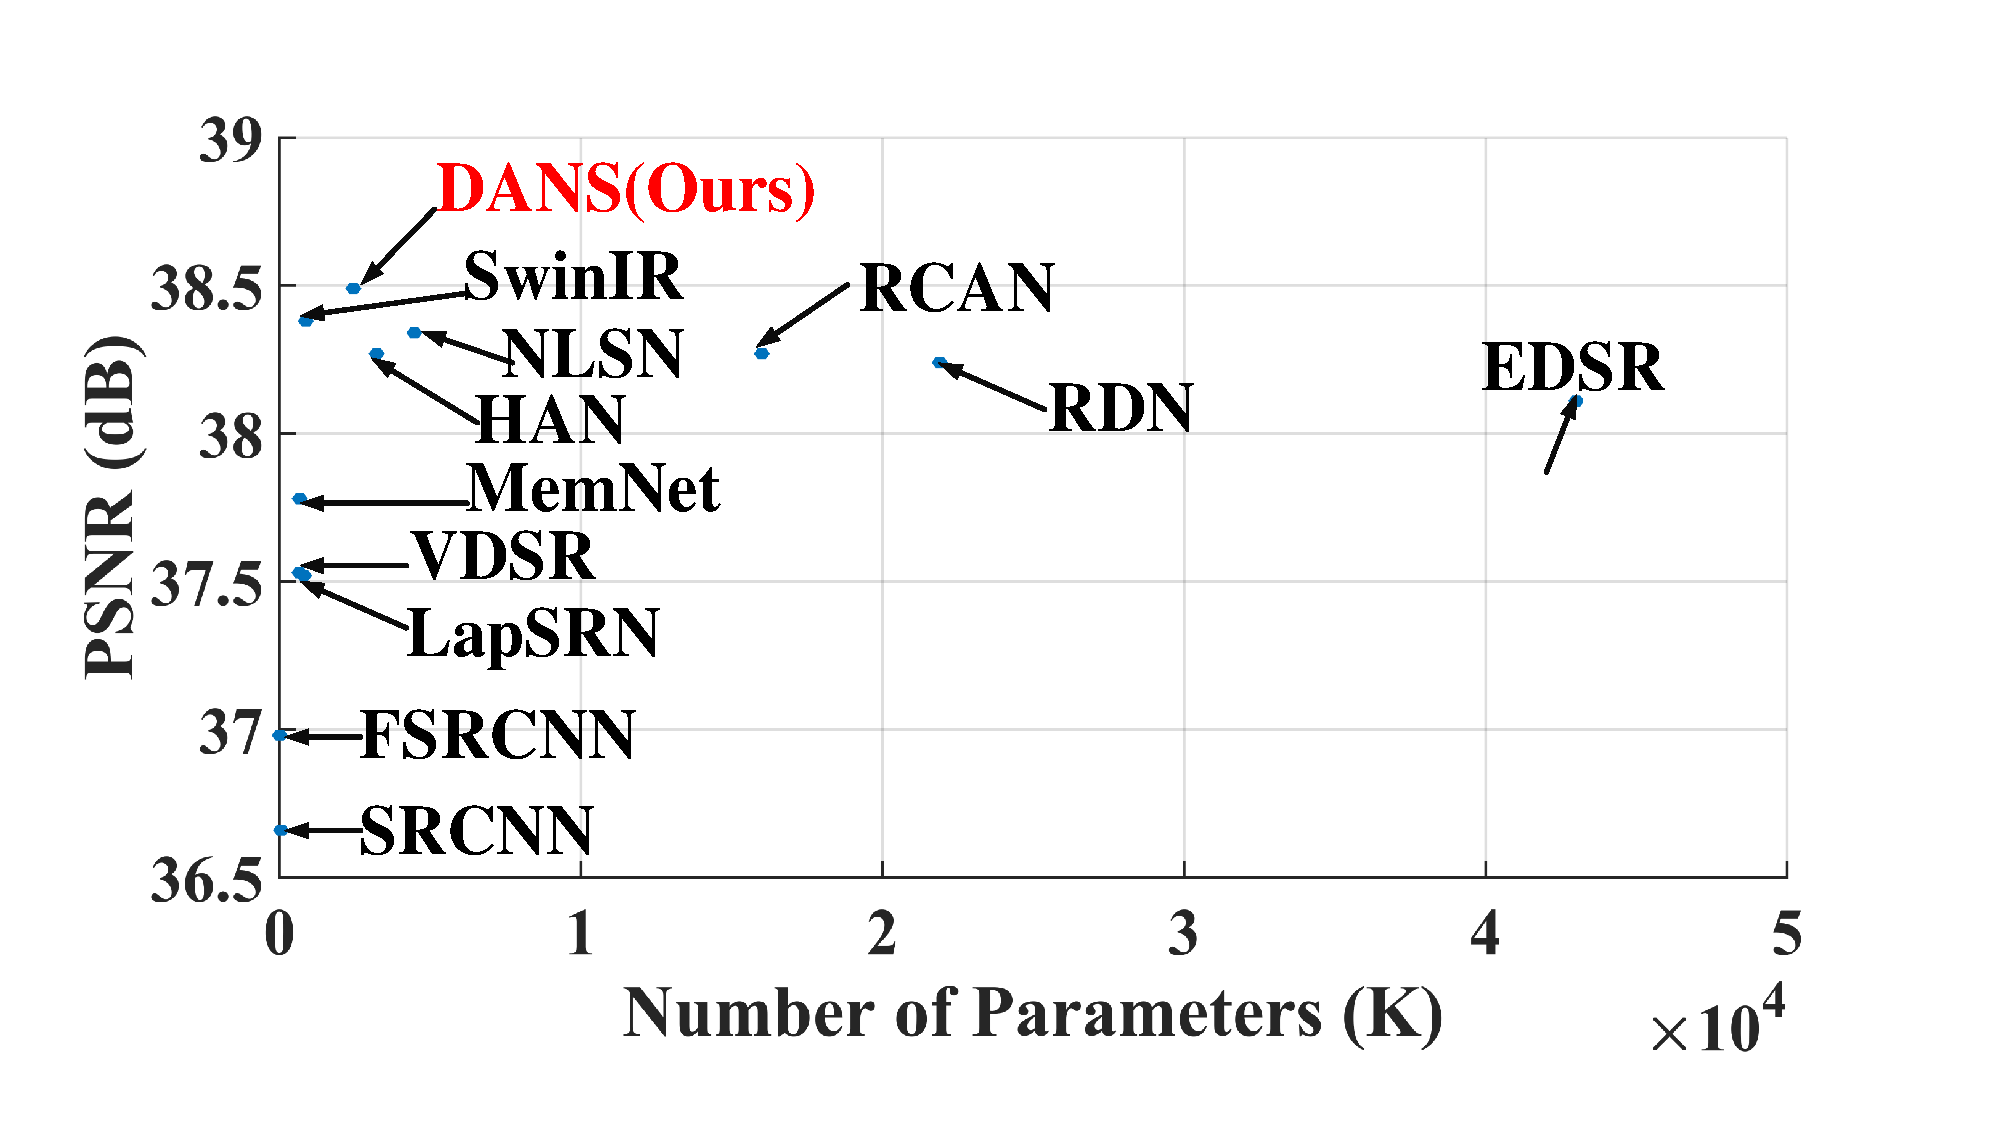
\includegraphics[width=\linewidth]{6FIGURE.pdf}
  \caption{Comparison of model parameters versus PSNR on the image dataset of Set5 [67] with enlargement factor $\times2$.}
  \label{fig:6}
\end{figure}

\subsection{Comparison analysis of PSNR and SSIM on the Image SR Datasets for enlargement factors of $\times$4 and $\times$8}

Figure	 7, Figure 8, Figure 9, and Figure 10 shows the performance comparison of different existing image SR methods using standard objective measures, i.e., PSNR and SSIM on benchmark datasets (Set5 [67], Set14 [68], BSD100 [69], Urban100 [70], Manga109 [71]) for enlargement factor of $\times4$ and $\times8$. The quantitative results reveal that our proposed DANS attains the most effective results as compared to NLSN [30], HAN [50], SwinIR [77], EDSR [22], and MemNet [43] on enlargement factor of $\times4$ and RCAN [19], HAN [50], RDN [73], DBPN [2] and AWSRN [78] on enlargement factor of $\times8$. The best improvement of our model for PSNR is shown in Set5 [67] and Manga109 [71] datasets at scale factor $\times4$, and for SSIM is shown in Manga109 [71] datasets at scale factor $\times8$.

\begin{figure}[ht]
  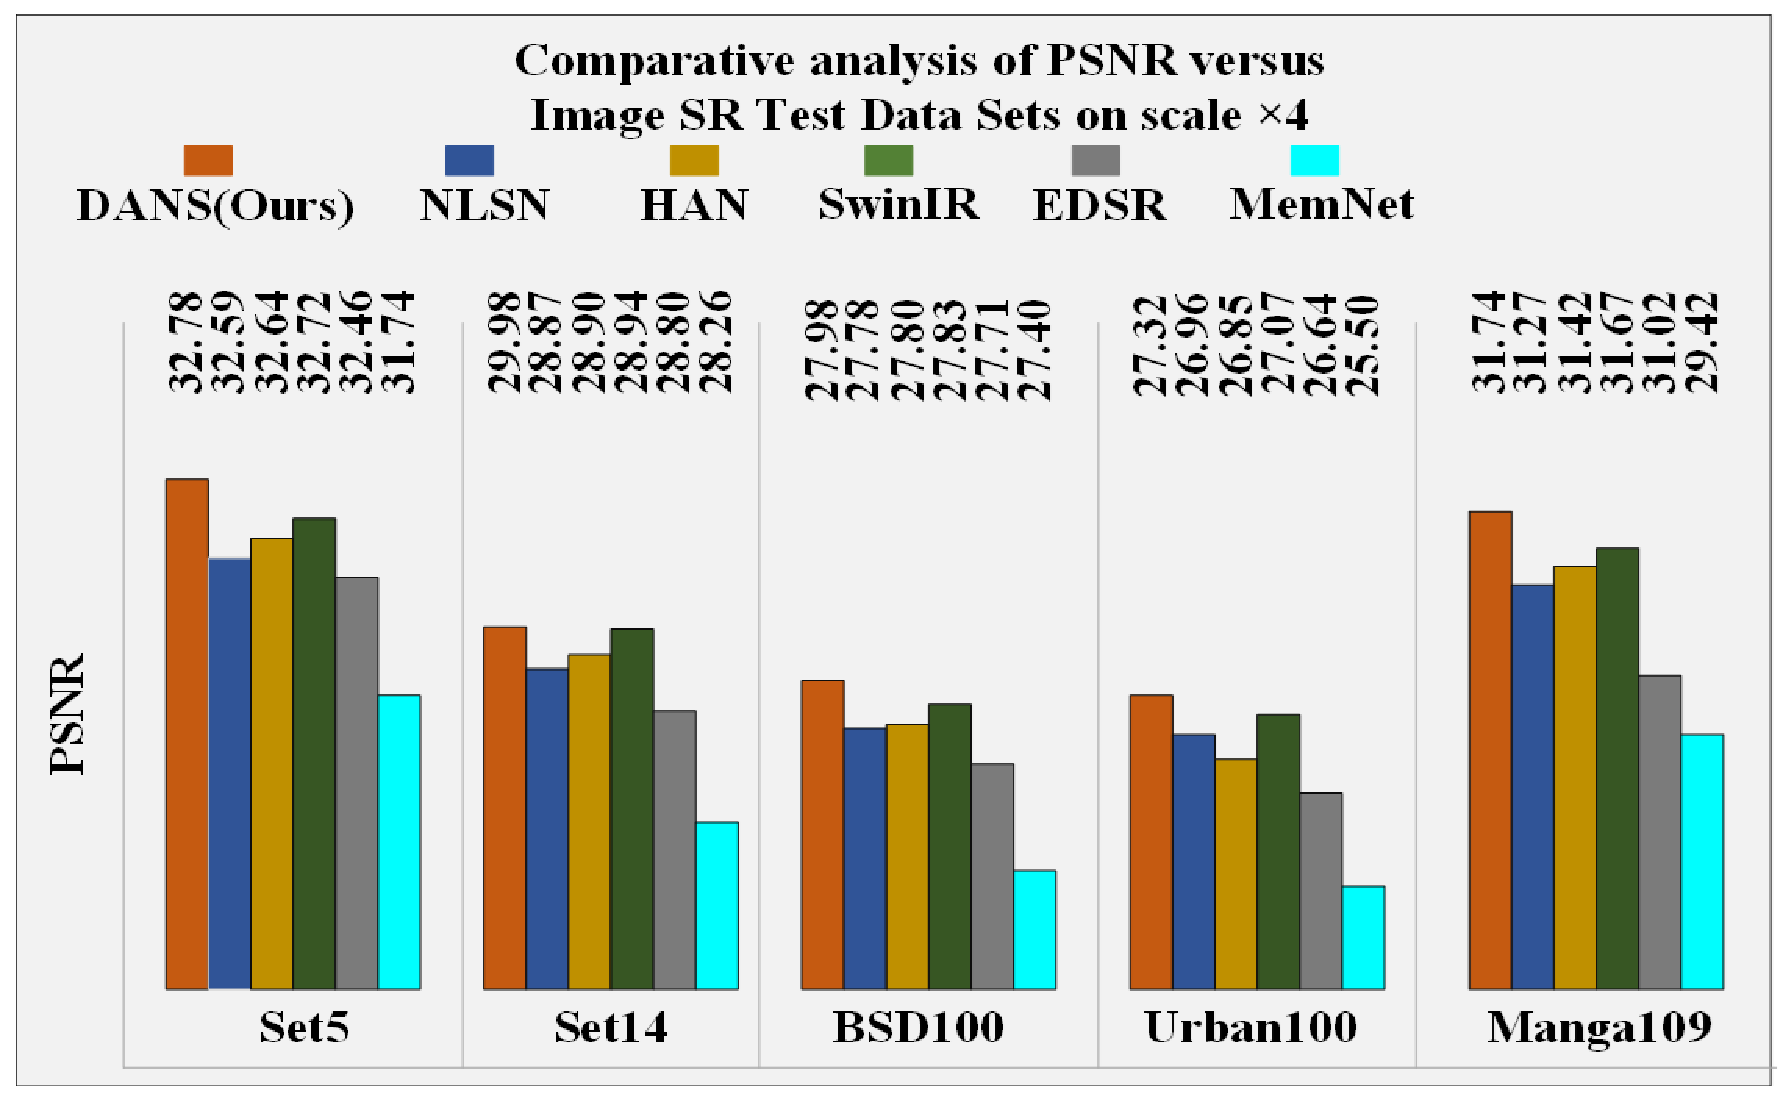
\includegraphics[width=\linewidth]{7FIGURE.pdf}
  \caption{Comparative analysis of PSNR versus Image SR Test Data Sets on enlargement factor $\times4$.}
  \label{fig:7}
\end{figure}

\begin{figure}[ht]
  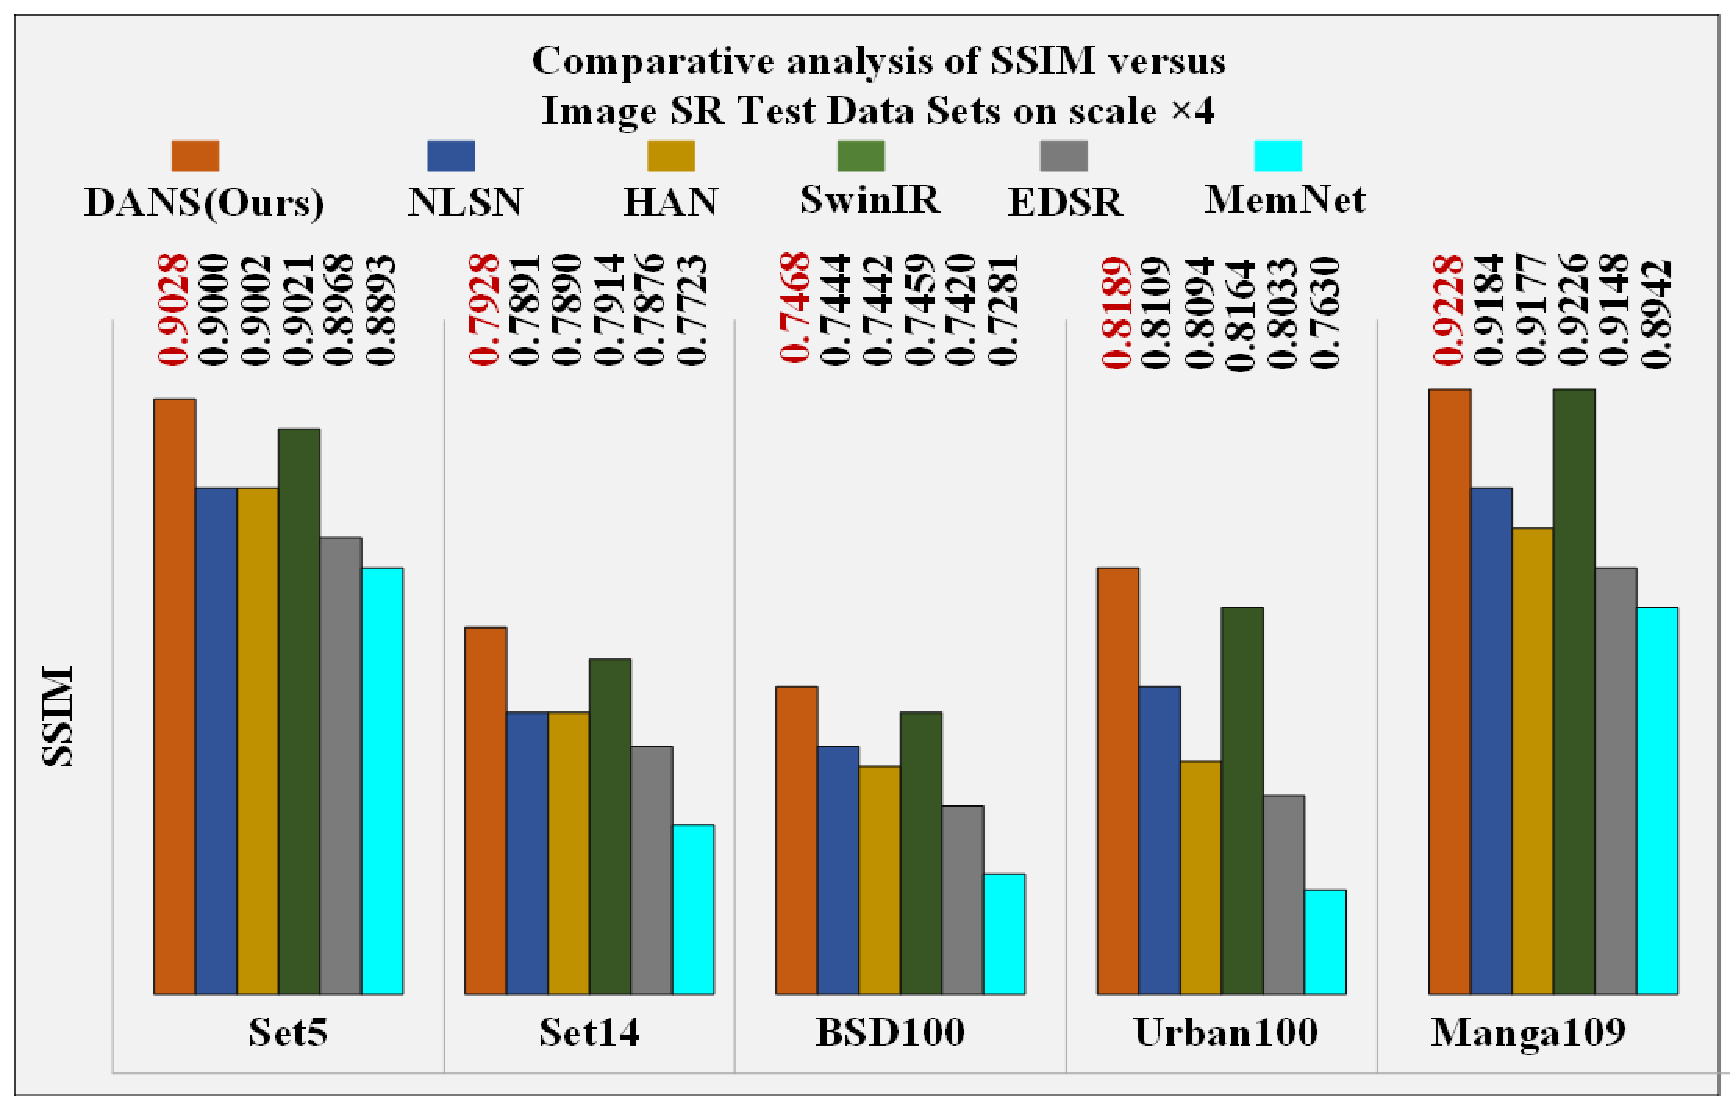
\includegraphics[width=\linewidth]{8FIGURE.pdf}
  \caption{Comparative analysis of SSIM versus Image SR Test Data Sets on enlargement factor $\times4$.}
  \label{fig:8}
\end{figure}

\begin{figure}[ht]
  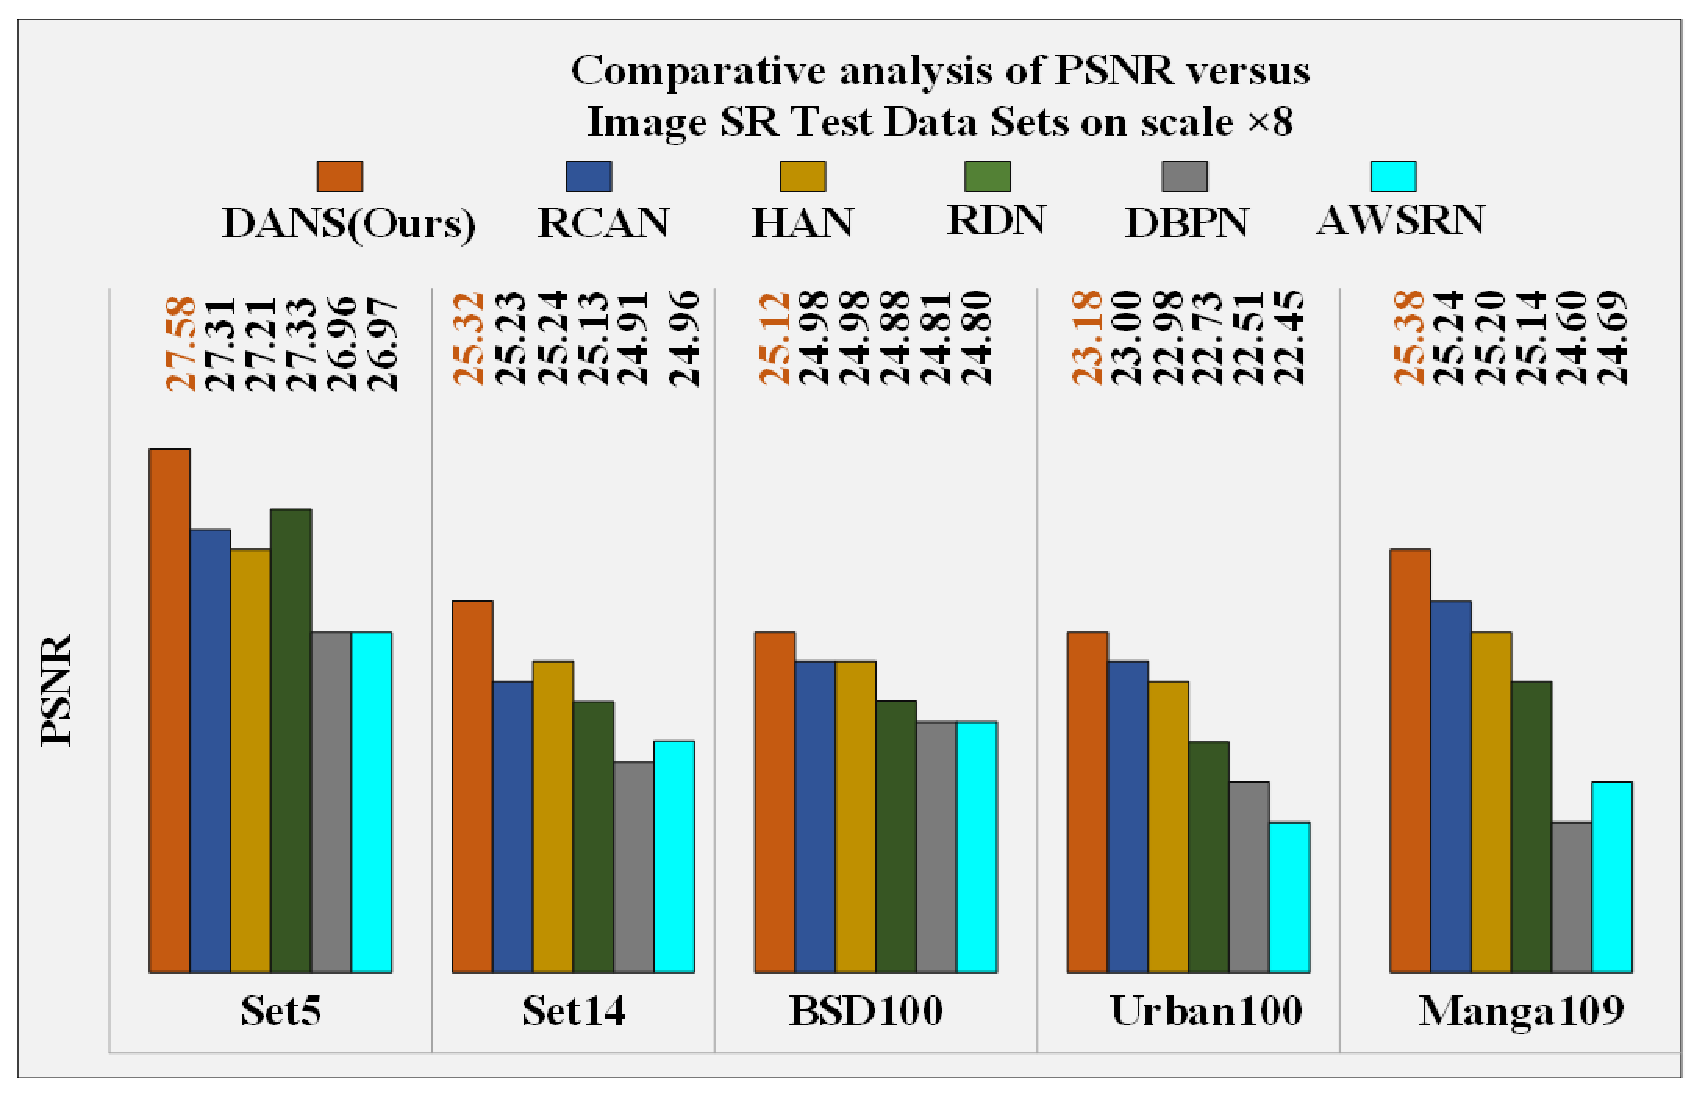
\includegraphics[width=\linewidth]{9FIGURE.pdf}
  \caption{Comparative analysis of PSNR versus Image SR Test Data Sets on enlargement factor $\times8$.}
  \label{fig:9}
\end{figure}

\begin{figure}[ht]
  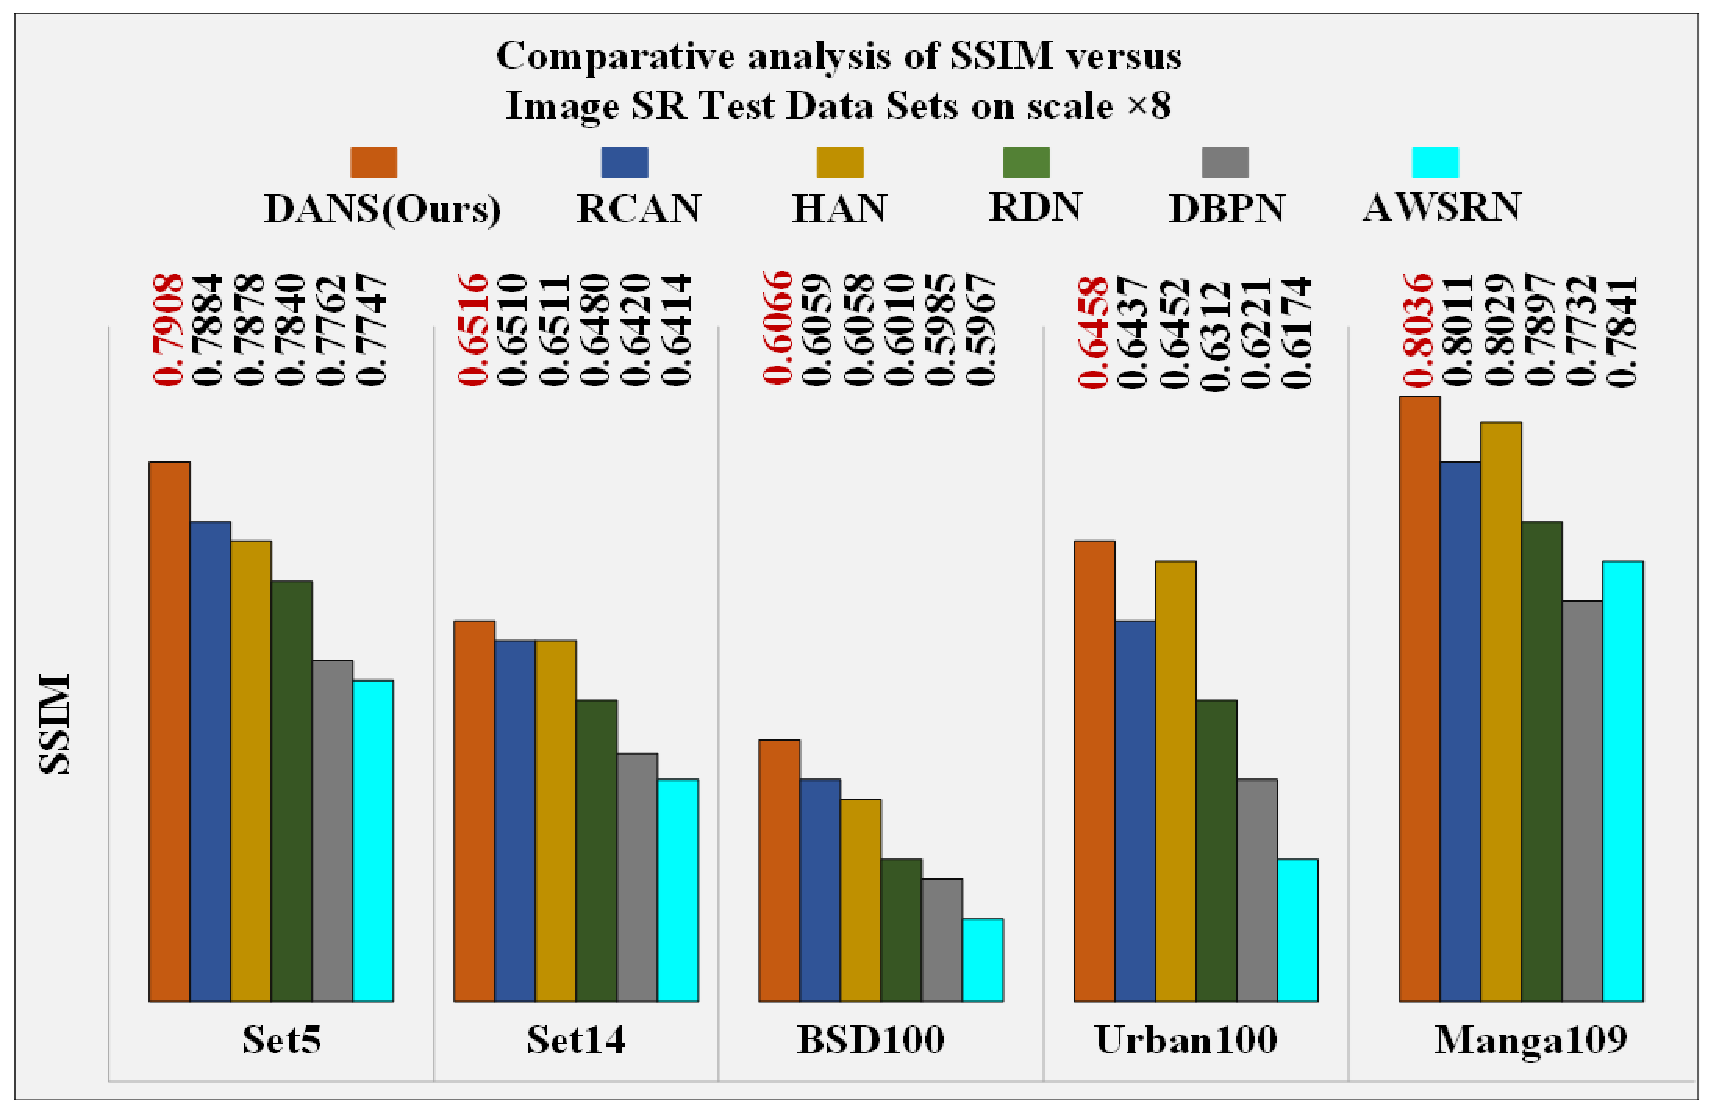
\includegraphics[width=\linewidth]{10FIGURE.pdf}
  \caption{Comparative analysis of SSIM versus Image SR Test Data Sets on enlargement factor $\times8$.}
  \label{fig:10}
\end{figure}

\subsection{Quantitative Analysis of PSNR versus execution time }
This section shows the performance of DANS regarding PSNR versus execution time, as shown in Figure 11. We used  NVIDIA GeForce GTX 2080ti GPU with 24GB memory to evaluate the state-of-the-art methods. For evaluation, GitHub codes provided by the research community have been used. Figure 11 shows the trade-off between  PSNR versus execution time on Set5 [67] scale factor $\times4$. Our proposed method gains the highest PSNR of 32.78 and is faster than five state-of-the-art methods (RCAN [19], EDSR [22], NLSN [30], MemNet [43], and VDSR [35]) except the SRCNN [17], FSRCNN [72] and LapSRN [74]. Furthermore, as seen in Figure 12, our proposed DANS has lesser computation costs regarding floating point operations (FLOPs).

\begin{figure}[ht]
  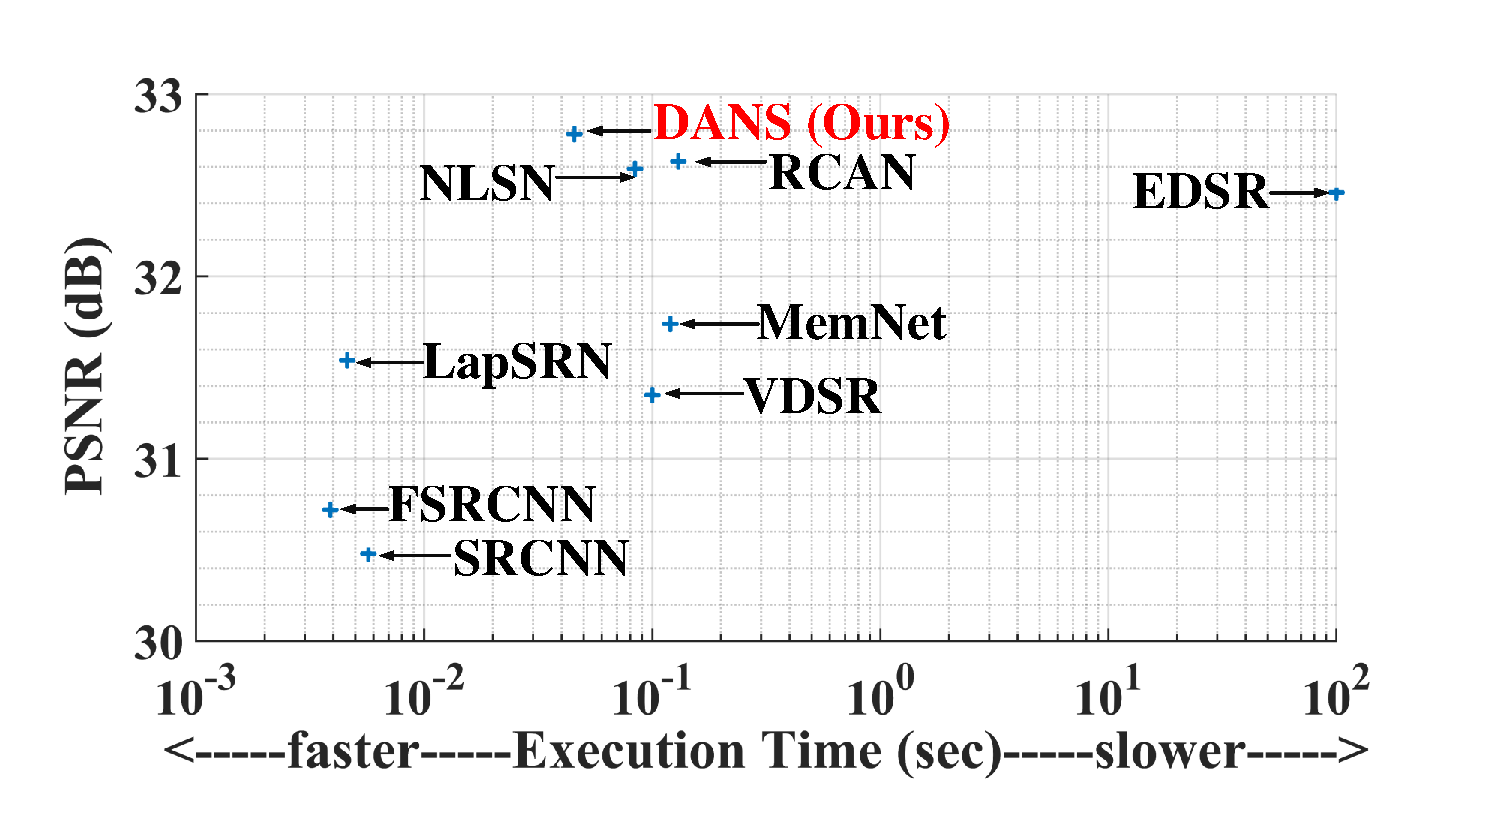
\includegraphics[width=\linewidth]{11FIGURE.pdf}
  \caption{Quantitative assessment of running time versus PSNR on Set5 [67] with scale factor $\times4$.}
  \label{fig:11}
\end{figure}

\begin{figure}[ht]
  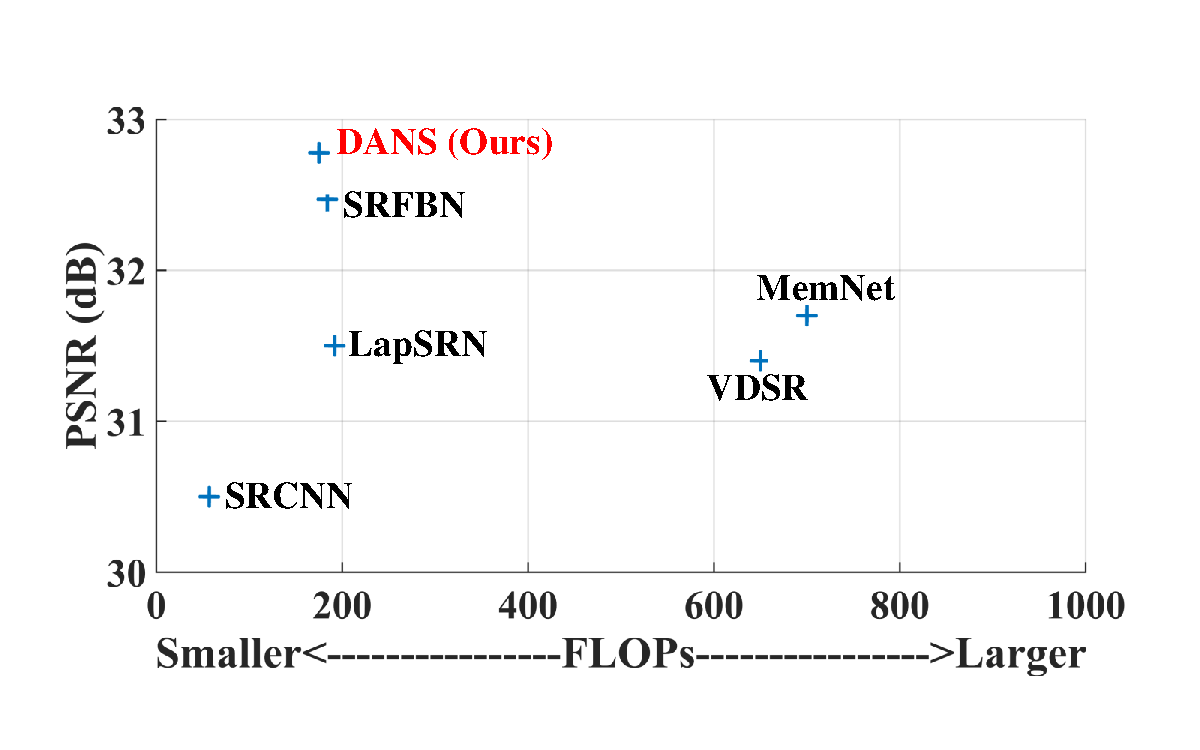
\includegraphics[width=\linewidth]{12FIGURE.pdf}
  \caption{Quantitative assessment of GFLOPs versus PSNR on Set5 [67] scale factor $\times4$.}
  \label{fig:12}
\end{figure}


\subsection{Performance  analysis of our model during training from the existing SR method}
In this subsection, we discuss performance evaluation during the training of our model. The average PSNR (dB) per epoch is shown in Figure 13, demonstrating that our model shows better training convergence than an existing SR model. The training hyperparameters are kept the same for a fair comparison. This evaluation is calculated for the training of enlargement factor of $\times4$ on the DIV2K [66] Dataset.


\begin{figure}[ht]
  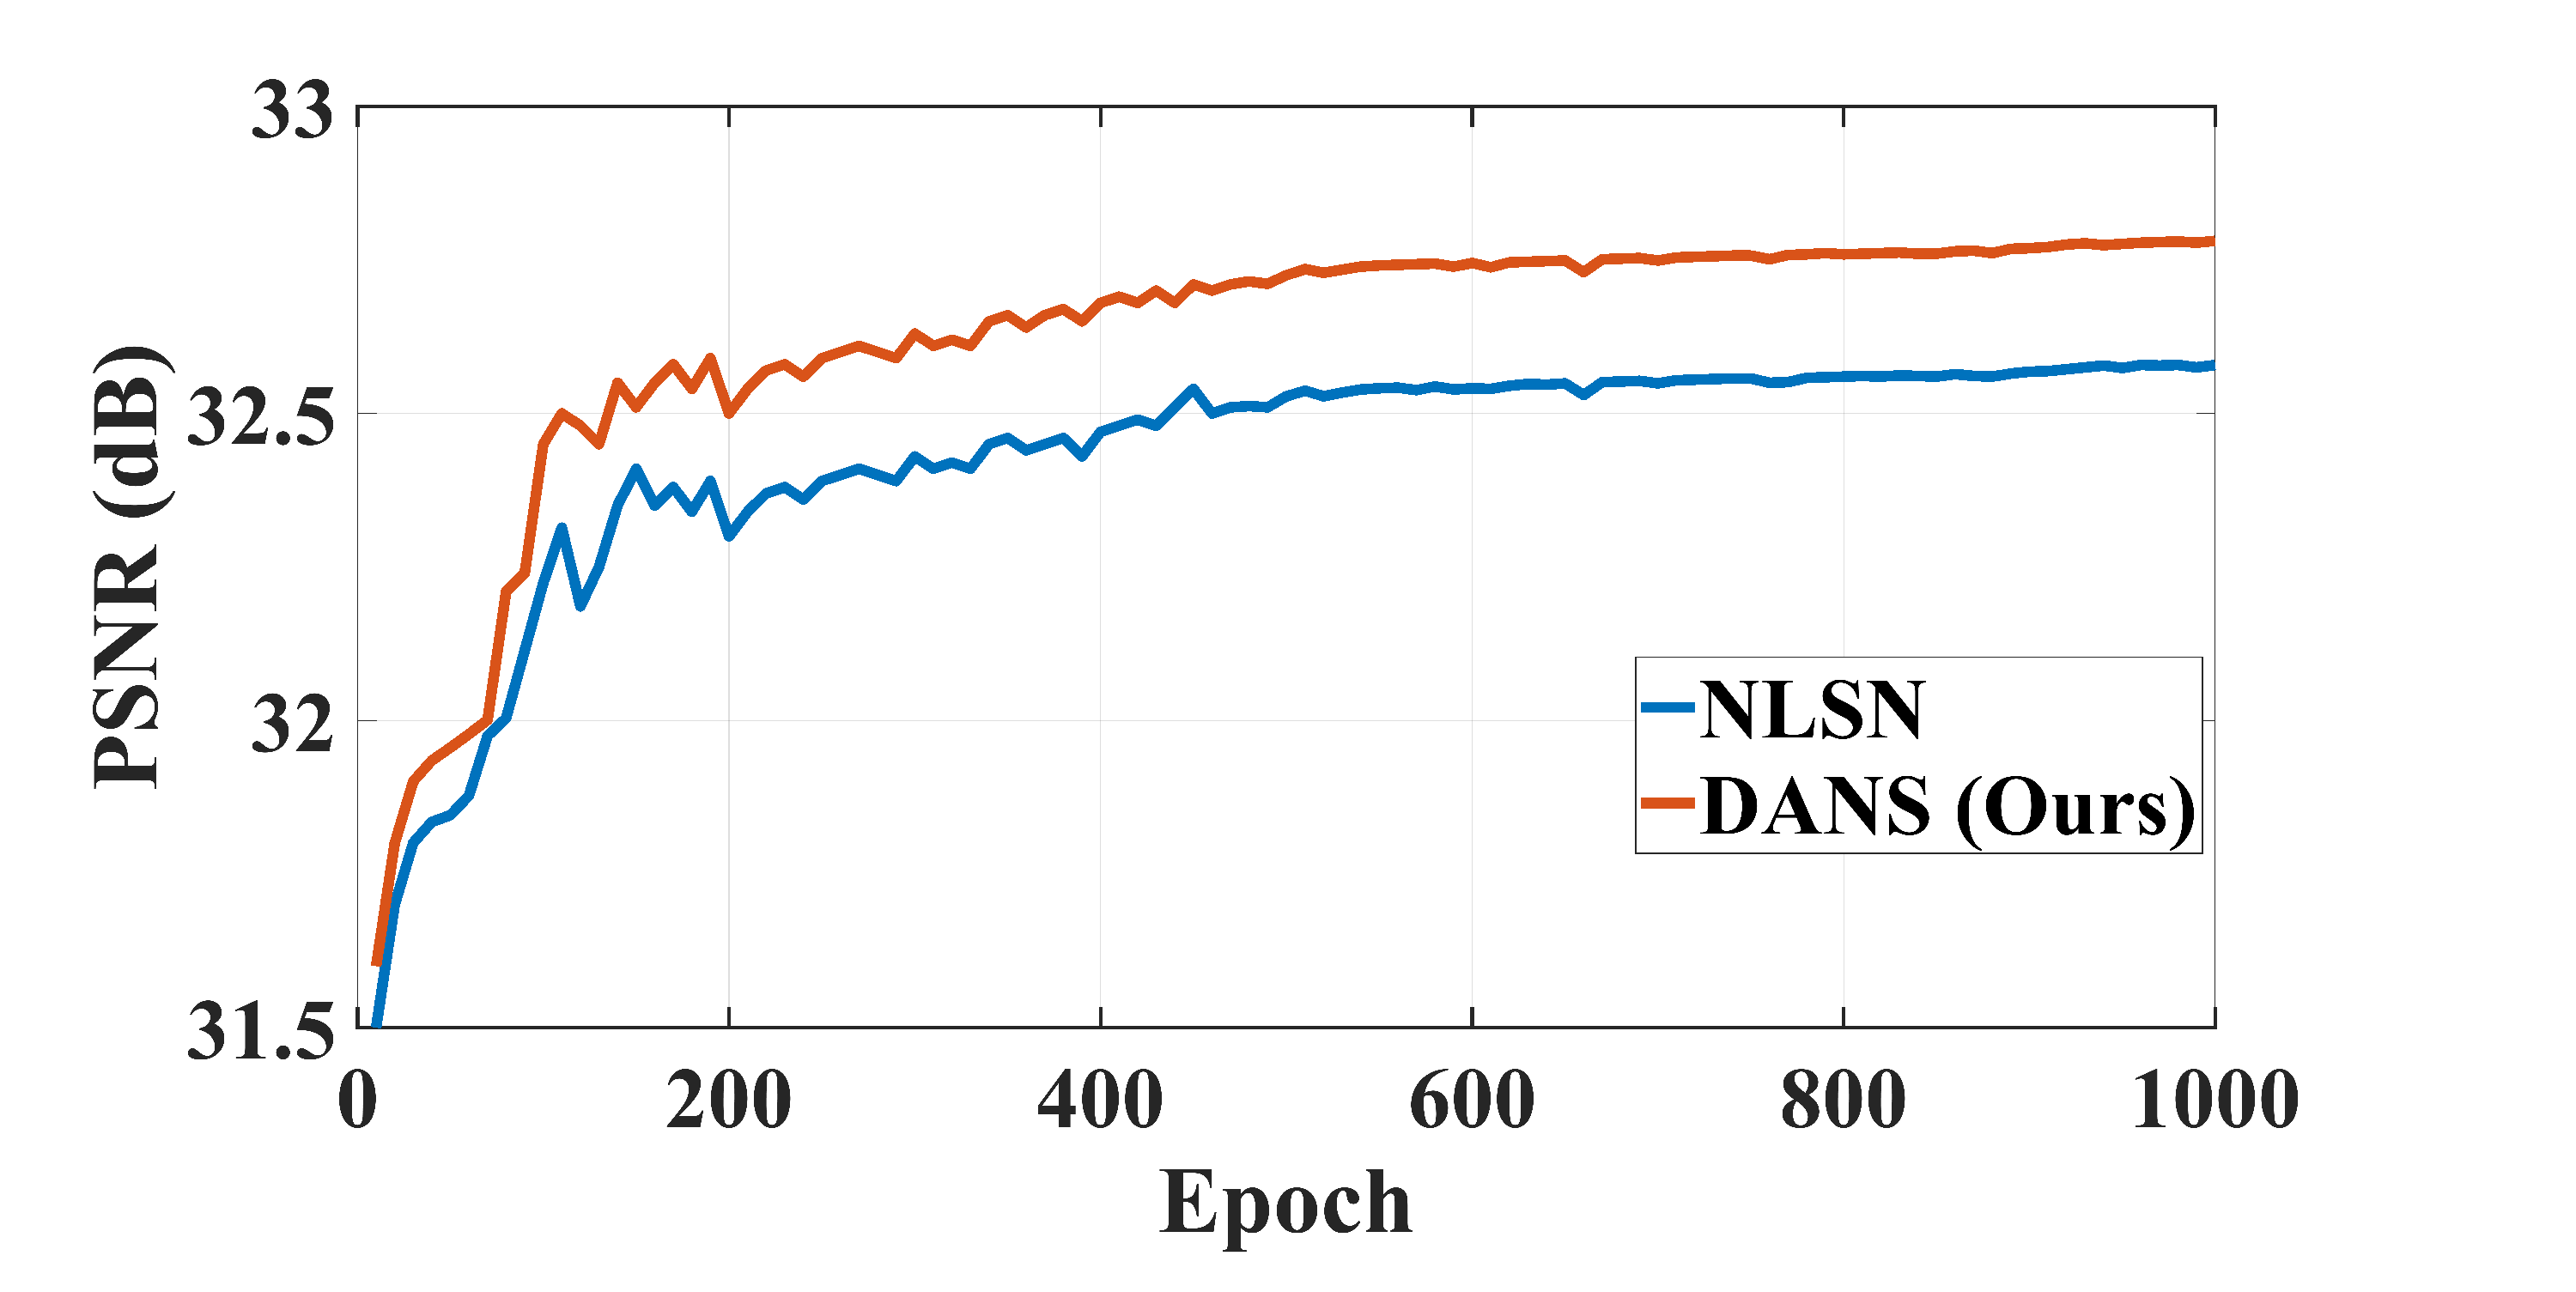
\includegraphics[width=\linewidth]{13FIGURE.pdf}
  \caption{Quantitative consideration of PSNR for an existing SR method on a scale factor $\times4$ on DIV2K [66] Dataset.}
  \label{fig:13}
\end{figure}

\subsection{Loss analysis of our model during training from the existing SR method}
This section describes the graph of the average training loss of our model. Figure 14 shows that our model shows better loss convergence than an existing SR model NLSN [30]. Our proposed DANS shows better and smoother convergence in an average loss in Figure 14 and average PSNR (dB) in Figure 13 during training. It is noted that average PSNR and loss are calculated for the training of scale $\times4$ on the DIV2K [66] dataset.

\begin{figure}[ht]
  \includegraphics[width=\linewidth]{14FIGURE.png}
  \caption{Loss versus epoch curve enlargement factor $\times$4 on DIV2K [66] dataset.}
  \label{fig:14}
\end{figure}

\subsection{Space Complexity Analysis}

An amount of memory space is required for an algorithm to operate on a computer. The space complexity of a deep CNN model represents how much memory it requires to run. The performance of a proposed algorithm establishes a balance between space and time (the complexity of space and time). In this section, we evaluate the space complexity on the publicly available Set5 test dataset with an enlargement factor of $\times$2. The space complexity of Set5 images such as baby, bird, butterfly, head, and woman are calculated with five state-of-the-art methods, including HR and LR images. Figure 15 shows that our proposed method has less space complexity (storage memory) than existing state-of-the-art methods.

\begin{figure}
  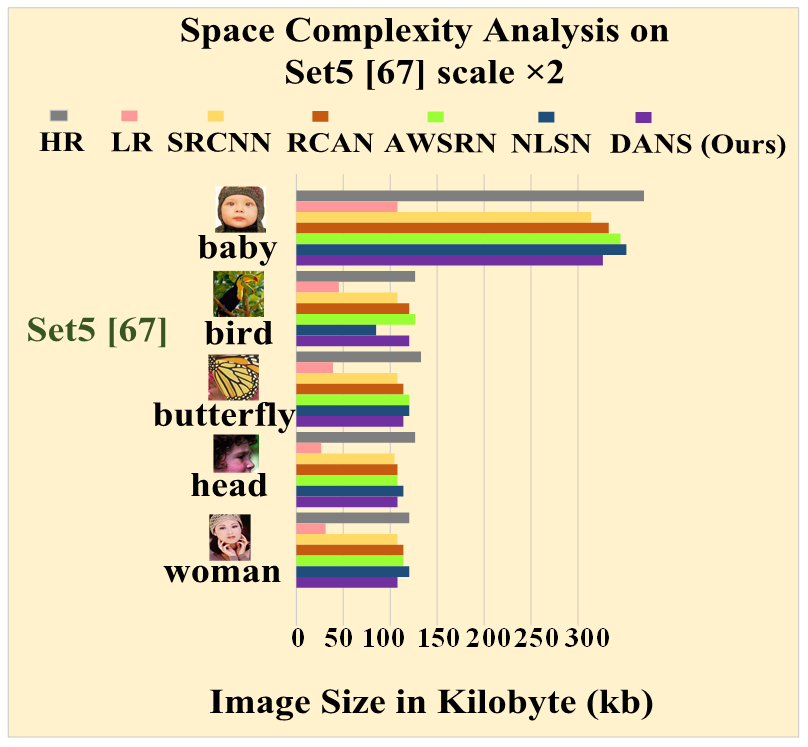
\includegraphics[width=\linewidth]{15FIGURE.png}
  \caption{Space complexity analysis for Set5 [67] Dataset images on scale factor $\times$2.}
  \label{fig:15}
\end{figure}

\subsection{Time Complexity Analysis}

The time required for completing each epoch during the training of a deep learning model demonstrates its complexity in terms of time. This is known as the time complexity of the DL model. In Figure 16, we show the time each epoch takes for 100 training epochs for an existing state-of-the-art method NLSN [30], and our proposed DANS. The curve shows a significant gap, indicating that our proposed DANS takes less training time for each epoch. Hence DANS show lesser time complexity than the baseline model.

\begin{figure}
  \includegraphics[width=\linewidth]{16FIGURE.png}
  \caption{Time complexity (Training time per epoch) for 100 epochs on DIV2K [66] Dataset images on scale factor $\times$4.}
  \label{fig:16}
\end{figure}

\subsection{Convergence Rate Analysis}

In deep learning, a model's convergence rate refers to how rapidly it can arrive at the best solution during training. It focuses on comprehending the learning algorithm's speed, time, and effectiveness for minimizing the loss during training. Figure 17 shows the convergence analysis for loss during training of the proposed DANS model for Set5 [67] scale ×4. Loss convergence of the model is calculated with different activations ReLU, PReLU and CReLU. As seen in Figure 17, ReLU shows a lesser loss convergence rate than CReLU and PreLU for our proposed DANS model. 

\begin{figure}
  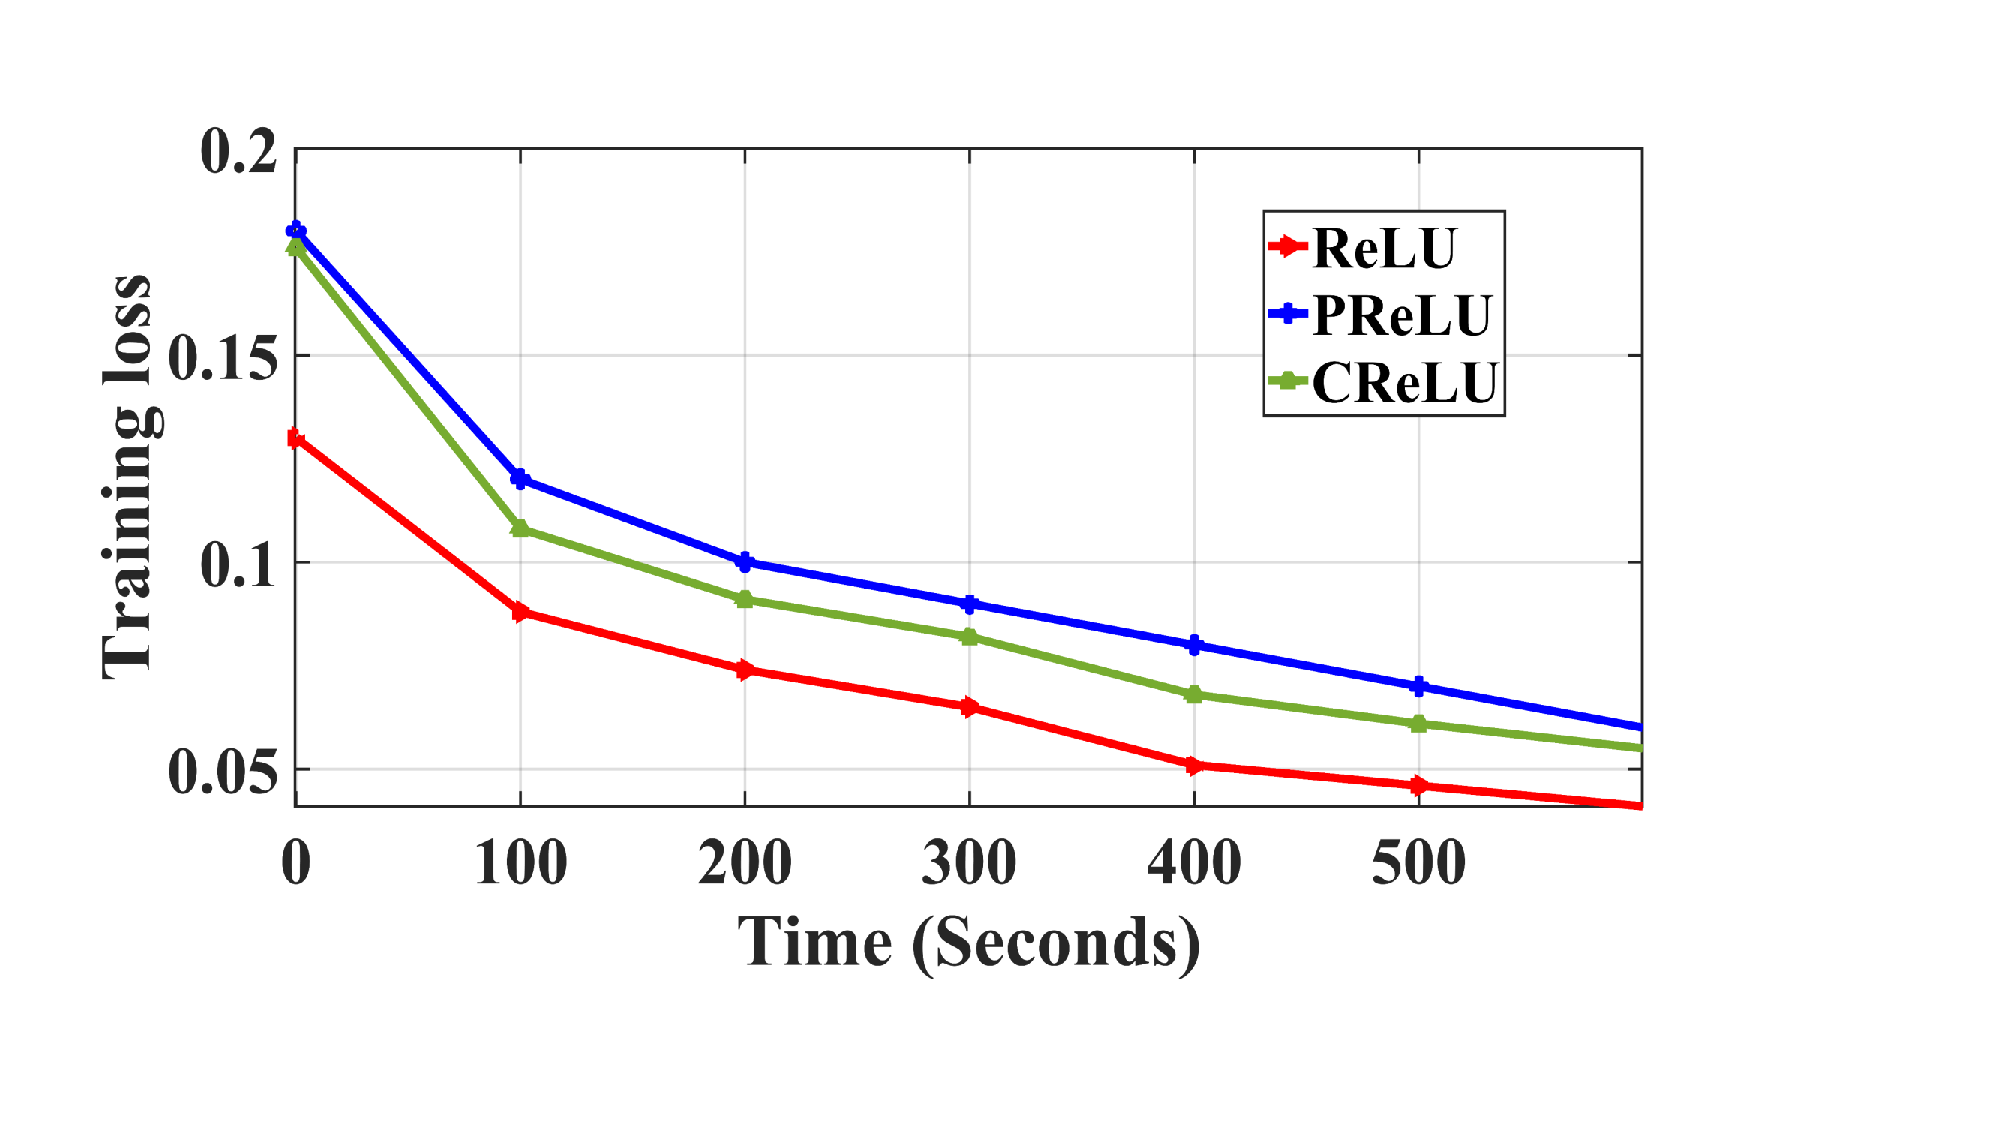
\includegraphics[width=\linewidth]{17FIGURE.pdf}
  \caption{Convergence rate analysis of proposed DANS for activactions on Set5 [67] for scale factor $\times$4.}
  \label{fig:17}
\end{figure}

Time complexity, space complexity, and convergence rate analyses are crucial to fully grasp the practical viability of an image super-resolution deep learning approach. These include the trade-off between computational demands, achievable performance, hardware accelerators (such as GPUs) for effective training, inference, and the available computing resources. When evaluating the practicality of an image super-resolution deep learning approach, examining the time complexity, space complexity, and convergence rate is helpful.


\subsection{Perceptual Quality Comparison}
Figure 18, Figure 19, Figure 20, Figure 21, Figure 22, Figure 23, and Figure 24 presents the visual quality of up-sampling factors $\times 4$ and $\times 8$ for image SR test datasets, including Set5 [67], Set14 [68], BSD100 [69], Urban100 [70] and Manga109 [71]. Blurry results are observed on up-sampling factor $\times 8$ for Bicubic, LapSRN [74], and MSRN [44]. Even though improving an image for an enlargement factor of $\times 8$ is difficult, our proposed DANS favorably reconstructs the fine contextual detail and constructively subdues the artifacts because of our encoder-decoder approach combined with Non-local sparse attention (NLSN) [30]. Non-local sparse attention (NLSN) [30] excels at capturing long-range dependencies and modeling global contextual details. Combining it with the encoder-decoder structure of U-Net [4] leads to increased discriminative [66] and informative feature representation both locally and globally. 
\newline

For enlargement factor $\times4$, we used the barbara image from Set14 [68] dataset, Img\_148026 from BSD100 [69], Img\_092 from Urban100 [70], and TaiyouNiSmash image from Manga109 [71] dataset. For enlargement factor $\times8$, we used Img\_253027 from BSD100 [69],  Img\_060 from Urban100 [70], and Hamlet image from Manga109 [71] dataset. Our proposed DANS shows visually pleasing patches and better quantitative metrics (PSNR/SSIM) as compared to other state-of-the-art methods such as Bicubic, MSRN [44], EDSR [22], AWSRN [78], RCAN [19], and NLSN [30] for $\times4$ and Bicubic, LapSRN [74], MSRN [44], DBPN [2], AWSRN [78], and RCAN [19] for enlargement factor of $\times8$. 

\begin{figure*}
    \centering

    \includegraphics[width=\linewidth]{18Figure.png}
    \caption{Qualitative improvement of Barbara image from Set14 [68] dataset on a scale factor of $\times4$.}
    \label{fig:18}
\end{figure*}

\begin{figure*}
    \centering

    \includegraphics[width=\linewidth]{19Figure.png}
    \caption{Qualitative improvement of image Img\_148026 from BSD100 [69] dataset on a scale factor $\times4$.}
    \label{fig:19}
\end{figure*}

\begin{figure*}
    \centering

    \includegraphics[width=\linewidth]{20Figure.png}
    \caption{Qualitative improvement of image Img\_092 from Urban100 [70] dataset on a scale factor $\times4$.}
    \label{fig:20}
\end{figure*}


\begin{figure*}
    \centering

    \includegraphics[width=\linewidth]{21Figure.png}
    \caption{Qualitative improvement of TaiyouNiSmash image from Manga109 [71] image dataset on a scale factor $\times4$.}
    \label{fig:21}
\end{figure*}


\begin{figure*}
    \centering

    \includegraphics[width=\linewidth]{22Figure.png}
    \caption{Qualitative improvement of Img\_253027 image from BSD100 [69] image dataset on scale factor of $\times8$.}
    \label{fig:22}
\end{figure*}

\begin{figure*}
    \centering

    \includegraphics[width=\linewidth]{23Figure.png}
    \caption{Qualitative improvement of Img\_060 image from Urban100 [70] image dataset on scale factor of $\times8$.}
    \label{fig:23}
\end{figure*}

\begin{figure*}
    \centering

    \includegraphics[width=\linewidth]{24Figure.png}
    \caption{Qualitative improvement of Hamlet image from Manga109 [71] image dataset on the scale factor $\times8$.}
    \label{fig:24}
\end{figure*}

\subsection{Ablation study}
In this section, we conduct controlled experiments to analyze our proposed model. The proposed model has six inception and 5 Non-local Sparse Attention (NLSA) blocks. We insert up-sampling and down-sampling with NLSA [30] block to give it an encoder-decoder [4] structure. Finally, we introduce a skip connection to the model to make it lightweight. The ablation study on the proposed model has been done in the following ways: (1) By changing activation functions to ReLU, PReLU, and CReLU in the inception block of the network design, (2) by changing the number of attention rounds on the Local Sensitivity Hashing technique inside the NLSA [30] block, (3) by noise degradation analysis of our proposed model using different activation at noise level 15 and degradation kernel is set to be 0.5, (4) by comparison analysis with traditional denoising techniques, and (5) by calculating Visual Information Fidelity (VIF). We conduct these experiments to check their effect on the performance of the proposed model. 

\subsubsection{Ablation study with different activation functions}

He \textit{et al.} [65] first introduced Parametric Rectified Linear Unit (PReLU) and Concatenated Rectified Linear Unit (CReLU). PReLU and CReLU have been introduced as extensions of ReLU to address its limitations. PReLU allows for more flexibility in the network by introducing a learnable parameter to provide a small negative slope for negative inputs. On the other hand, CReLU concatenates ReLU with ReLU-like functions with negative slopes, providing a more complex activation function. Henceforth, we attempt to change the activation function inside the inception block in the proposed model to check its effect on performance. Figure 25 shows the activation function has been changed inside the inception block of the model to see the impact on performance. 

The ReLU activation function is known for its simplicity, computational efficiency, and better sparsity. Even though PReLU and CReLU are advancements over ReLU, they cannot provide better sparsity than ReLU. This has been demonstrated by evaluating PSNR for different designs of models having inception blocks with ReLU, PReLU, and CReLU in Table 3. The red color demonstrates the best value, and the blue underlined demonstrates the second-best value. It can be observed in Figure 26 that ReLU shows better convergence as compared to PReLU and CReLU when it comes to dealing with sparsity.
\begin{figure}[H]
  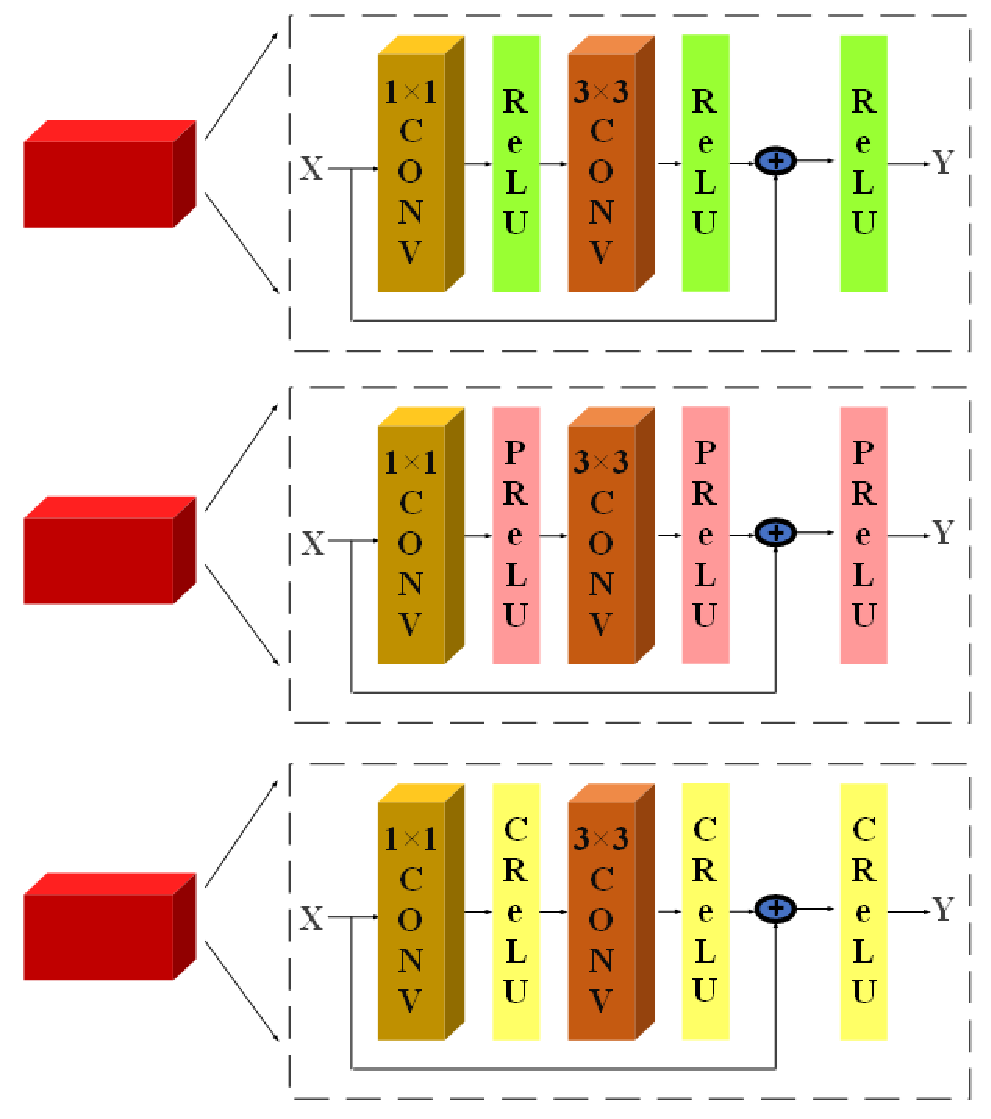
\includegraphics[width=\linewidth]{25FIGURE.pdf}
  \caption{Inception Block with different activations.}
  \label{fig:25}
\end{figure}
 
\begin{table} 
\caption{Ablation study of different activations in inception blocks, including ReLU, CReLU, and PReLU. The quantitative value of average PSNR calculated on Set5 [67] enlargement factor $\times4$  on 50 epochs. The best quantitative value has been recorded as bold with {\color{red}\textbf{Red }} color. The second-best quantitative value is shown in {\color{blue}\underline{blue}} color with an underline.}
\label{table3}
\setlength{\tabcolsep}{3pt}
\centering
\begin{tabular}{|c|c|c|c|c|}
\hline
Activation Function      & \multicolumn{3}{c|}{Inception Block}    & Average PSNR                \\
\hline
ReLU         & \checkmark & $\times$ &$\times$  &{\color{red}\textbf{32.56}}   \\
\hline
PReLU          &$\times$& \checkmark& $\times$  & {\color{blue}\underline{32.50}}  \\
\hline
CReLU          &$\times$& $\times$ & \checkmark  & {32.39}   \\

\hline
\end{tabular}
\end{table}



\begin{figure}
  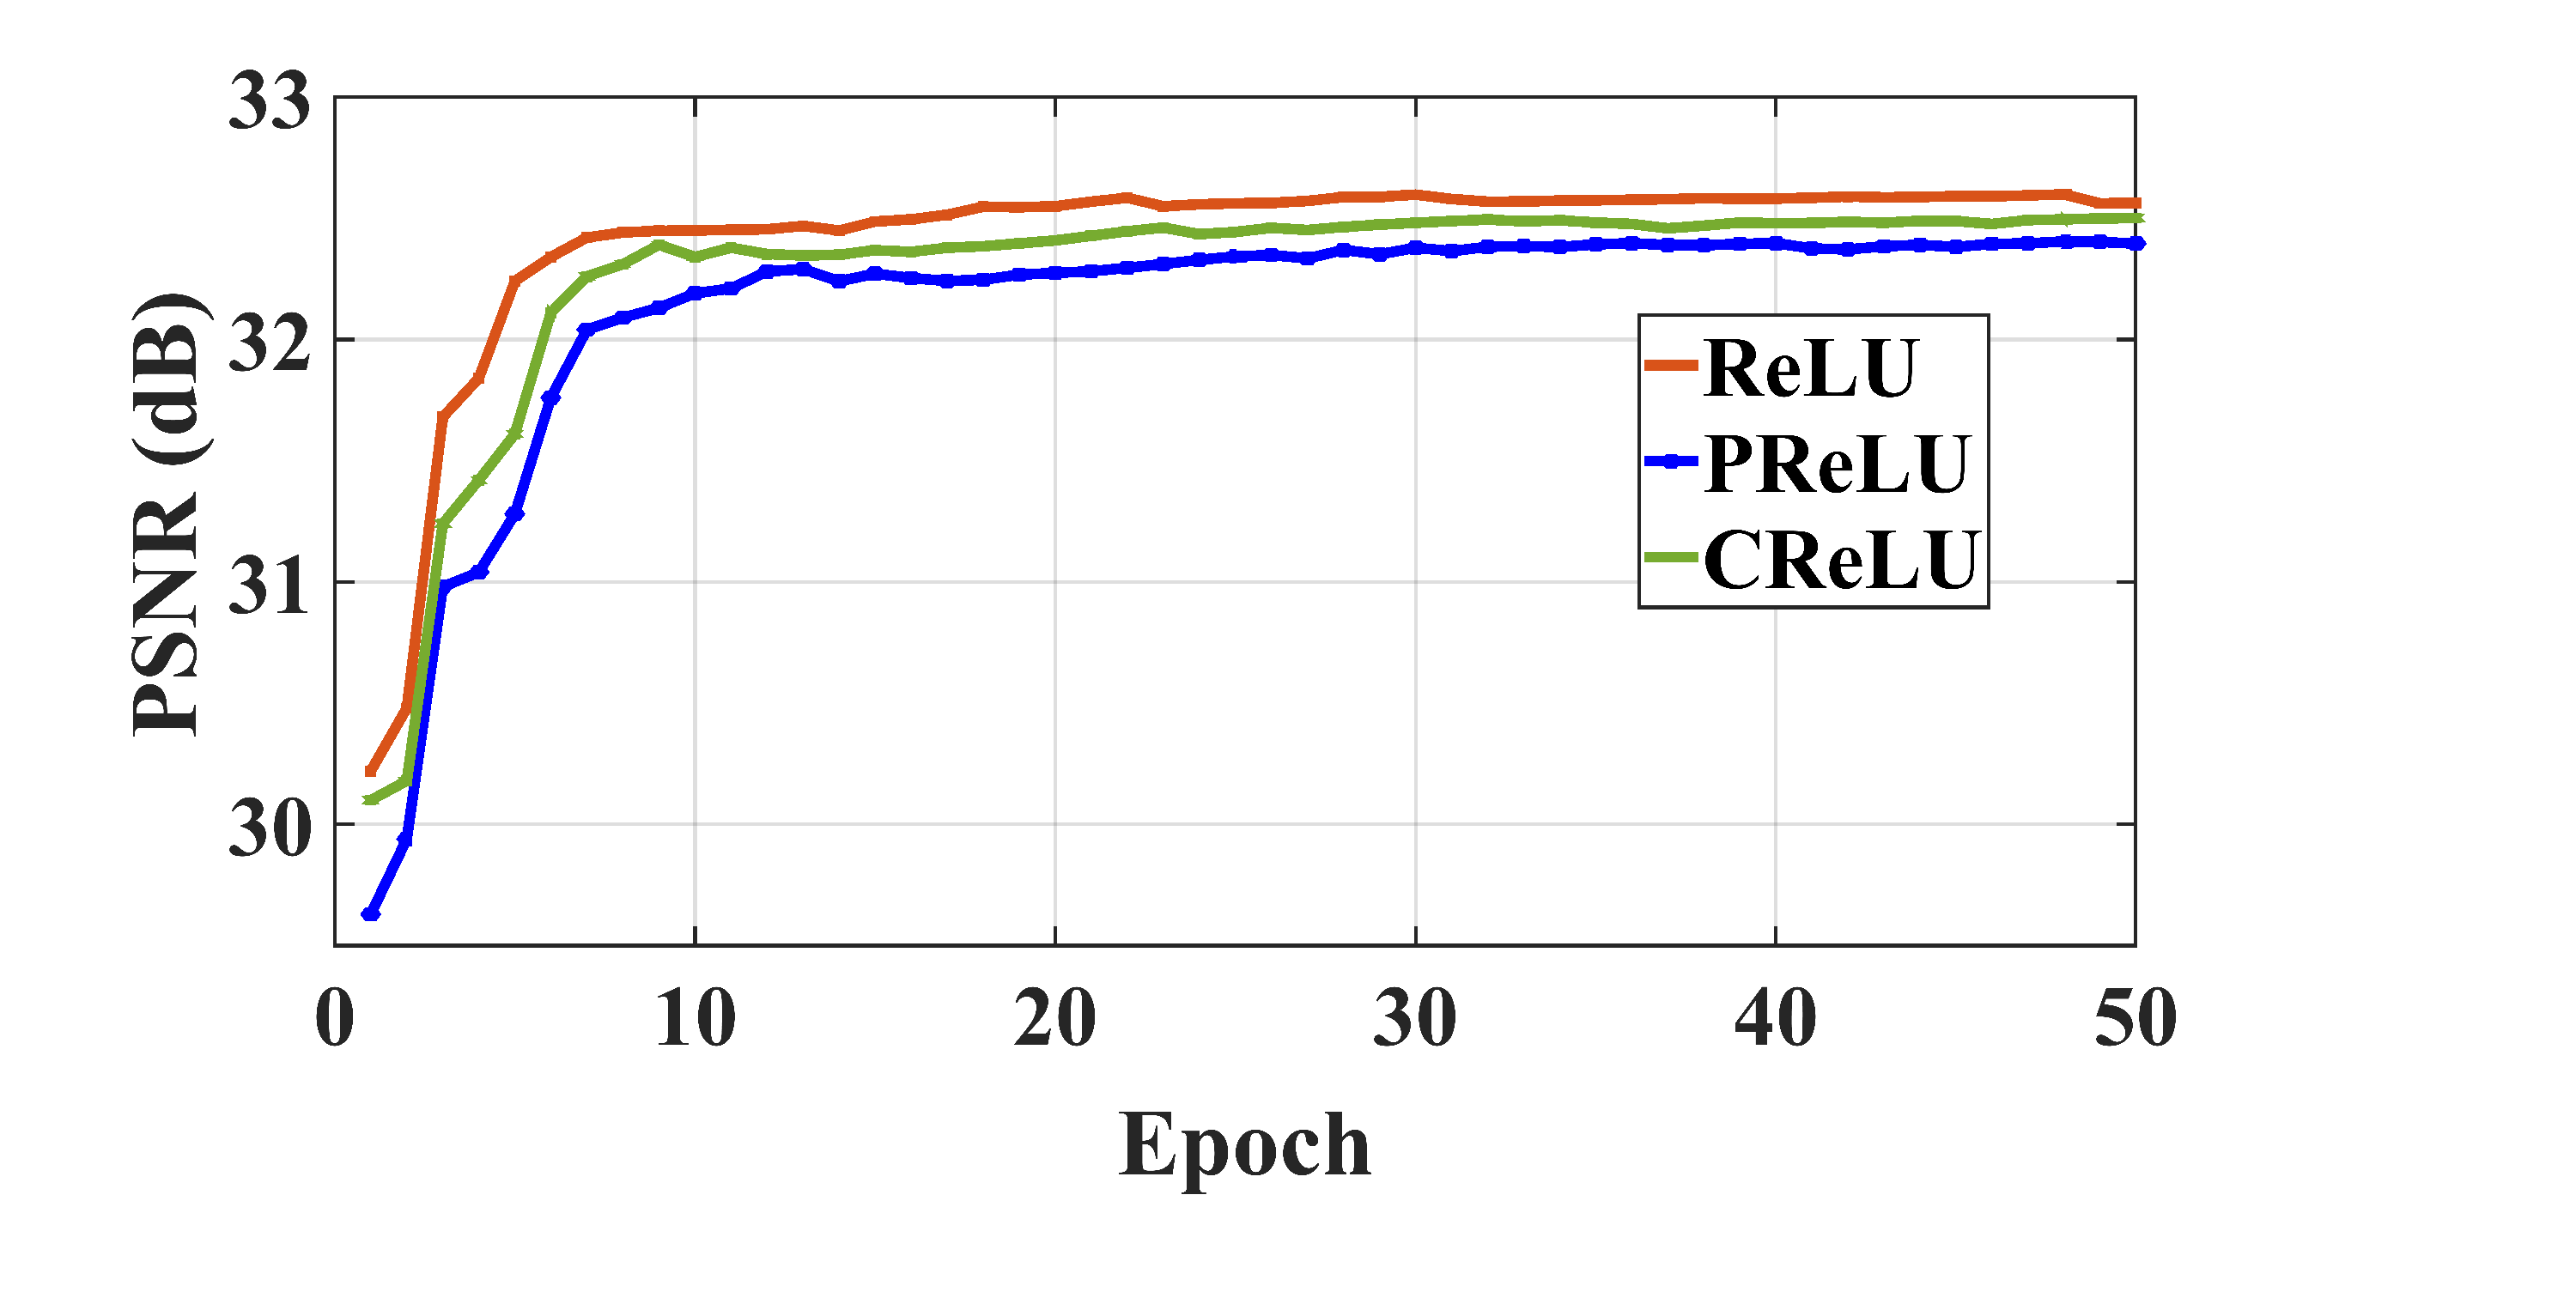
\includegraphics[width=\linewidth]{26FIGURE.pdf}
  \caption{Performance assessment of PSNR (dB) versus training epoch for different activations on enlargement factor $\times$4 on Set5 [67].}
  \label{fig:26}
\end{figure}

Table 3 shows that ReLU gives better PSNR on an average calculated on Set5 [67] for enlargement factor $\times4$ compared to PReLU and CReLU. Since ReLU is computationally efficient, as shown in Figure 26, the network with ReLU activation converges better. It helps the network train faster than those with PReLU and CReLU. 

\subsubsection{Ablation Study with different rounds of Attention in Non-Local Sparse Attention Blocks}
Since the Local Sensitivity Hashing (LSH) [80] technique used in NLSA [30] works on improving the robustness of the model, its computational cost is furthermore reduced by adjusting the attention rounds \textit{r}. Table 4 shows the result of the model trained and evaluated for different attention rounds. This result indicates that increasing the number of hashing rounds either at training or evaluation improves the accuracy of the super-resolution model. As a result, the best performance in terms of PSNR is achieved at the highest value, i.e., 8 for hashing rounds. Figure 27 shows the effect of attention rounds for r = 4 and r = 8 on the benchmark dataset for an enlargement factor of $\times$ 2.


\begin{table*}
\centering
\caption{Effect of different attention rounds on performance for enlargement factor of $\times$2. The best quantitative value has been recorded as bold with {\color{red}\textbf{Red }} color. The second best quantitative value is shown in {\color{blue}\underline{blue}} color with an underline.}

\label{table4}
\setlength{\tabcolsep}{3 pt}
\begin{tabular}{|c|cc|cc|cc|cc|cc|}
\hline
\multirow{2}{*}{Non-Local attention rounds} & \multicolumn{2}{c|}{Set5 [67]} & \multicolumn{2}{c|}{Set14 [68]} & \multicolumn{2}{c|}{BSD100 [69]} & \multicolumn{2}{c|}{Urban100 [70]} & \multicolumn{2}{c|}{Manga109 [71]}    \\

\cline{2-11}& \multicolumn{1}{c|}{NLSN}  & DANS   & \multicolumn{1}{c|}{NLSN} & DANS    & \multicolumn{1}{c|}{NLSN} & DANS    & \multicolumn{1}{c|}{NLSN}  & DANS  & \multicolumn{1}{c|}{NLSN}  & DANS     \\
\hline


r=1 &\multicolumn {1}{c|}{37.87 } & 37.92  &\multicolumn {1}{c|}{33.76 } & 33.81 &\multicolumn {1}{c|}{31.38 } & 31.44 &\multicolumn {1}{c|}{32.26 } & 32.28 &\multicolumn {1}{c|}{38.36 } & 38.40 \\

r=2 &\multicolumn {1}{c|}{37.90 } & 37.96  &\multicolumn {1}{c|}{33.80 } & 33.84 &\multicolumn {1}{c|}{31.42 } & 31.48 &\multicolumn {1}{c|}{32.30 } & 32.33 &\multicolumn {1}{c|}{38.37 } & 38.42 \\

r=4 &\multicolumn {1}{c|}{37.92} & {\color{blue}\underline{37.99}}  &\multicolumn {1}{c|}{33.86} & {\color{blue}\underline{33.90}} &\multicolumn {1}{c|}{31.47} & {\color{blue}\underline{31.52}} &\multicolumn {1}{c|}{32.32} & {\color{blue}\underline{32.36}} &\multicolumn {1}{c|}{38.40} & {\color{blue}\underline{38.44}} \\

r=8 &\multicolumn {1}{c|}{37.93} & {\color{red}\textbf{38.08}}  &\multicolumn {1}{c|}{33.89} & {\color{red}\textbf{33.94}} &\multicolumn {1}{c|}{31.50} & {\color{red}\textbf{31.53}} &\multicolumn {1}{c|}{32.35} & {\color{red}\textbf{32.38}} &\multicolumn {1}{c|}{38.43} & {\color{red}\textbf{38.46}} \\



\hline



\end{tabular}
\end{table*}

\begin{figure}
  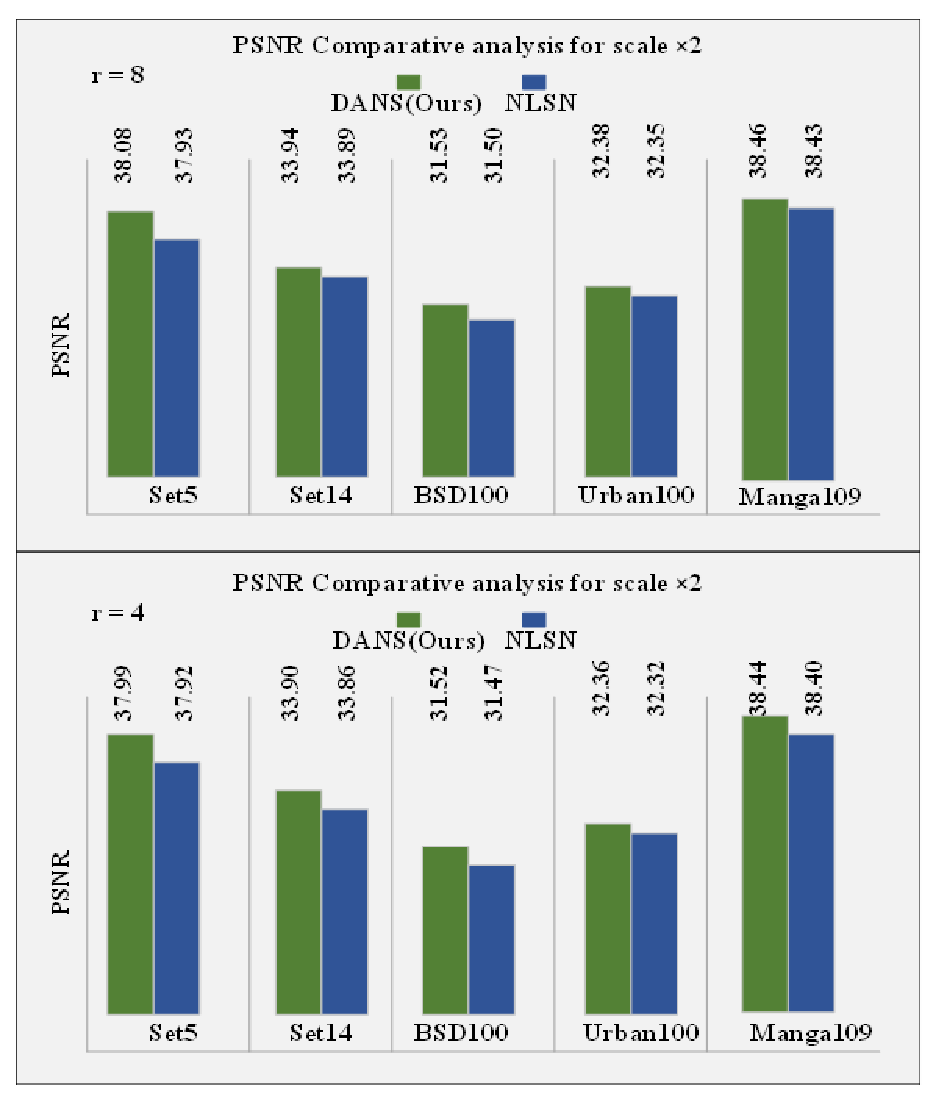
\includegraphics[width=\linewidth]{27FIGURE.pdf}
  \caption{Performance assessment of PSNR (dB) versus image dataset for different rounds of activations on enlargement factor $\times$2.}
  \label{fig:27}
\end{figure}

\subsubsection{Noise Degradation Analysis of the proposed model}

Performance evaluation using different activations, i.e., ReLU, PReLU, and CReLU, has been demonstrated in Table 5 on Set5 [67] for enlargement factors $\times$2 and $\times$4, respectively. Gaussian noise has been added to the image keeping the noise level at 15, and the degradation kernel is set to 0.5. Table 5 shows that our proposed model performs better for noise-degraded images and can be used as a denoiser [79].


\begin{table} 
\centering
\caption{Quantitative evaluation of different activations on noise degradation of images on Set5 [67] for enlargement factors of $\times$2 and $\times$4. The best quantitative value has been recorded as bold with {\color{red}\textbf{Red }} color. The second best quantitative value is shown in {\color{blue}\underline{blue}} color with an underline.}

\label{table5}
\setlength{\tabcolsep}{3 pt}
\begin{tabular}{|c|c|cc|}
\hline
\multirow{2}{*}{Methods} & \multirow{2}{*}{Factor} & \multicolumn{2}{c|}{Set5 [67]}  \\

\cline{3-4}&& \multicolumn{1}{c|}{PSNR}  & SSIM        \\

\hline

DANS (with PReLU) &$\times2$ &\multicolumn {1}{c|}{28.61 } & 0.6804  \\

DANS (with CReLU) &$\times2$ &\multicolumn {1}{c|}{\color{blue}\underline{28.86}} & {\color{blue}\underline{0.6838}}  \\

DANS (with ReLU) &$\times2$ &\multicolumn {1}{c|}{\color{red}\textbf{28.94}} & {\color{red}\textbf{0.6842}}  \\

\hline

DANS (with PReLU) &$\times4$ &\multicolumn {1}{c|}{23.34 } & 0.4694  \\

DANS (with CReLU) &$\times4$ &\multicolumn {1}{c|}{\color{blue}\underline{23.52}} & {\color{blue}\underline{0.4712}}  \\

DANS (with ReLU) &$\times4$ &\multicolumn {1}{c|}{\color{red}\textbf{23.68}} & {\color{red}\textbf{0.4742}}  \\

\hline

\end{tabular}
\end{table}

Table 5 shows that ReLU performs better in terms of PSNR and SSIM for noise-degraded images than PReLU and CReLU activation. Since ReLU promotes sparsity in activations, it shows the best performance. The red color indicates the best performance, and blue with an underline indicates the second-best. The high PSNR and SSIM show the robustness of ReLU against noise degradation in the proposed model. 

\subsubsection{Comparison Analysis with traditional denoising techniques}

In this section, we show the comparison of our proposed DANS model on Set14 [68] Dataset on scale $\times$4 with classical denoising methods such as Block Matching and 3D Filtering (BM3D) [81], Weighted Nuclear Norm Minimization with Application to Image Denoising (WNNM) [82], Denoising Convolutional Neural Network (DnCNN) [38], Fast and Flexible Solution for CNN-Based Image Denoising (FFDNet) [83] and Nonlocally centralized sparse representation for image restoration (NCSR) [84]. Performance comparison in terms of PSNR is shown using Gaussian noise keeping noise level ($\sigma$), i.e., $\sigma = 5$, $\sigma = 10$ and $\sigma = 15$ in Table 6. It can be observed from Table 6 that our proposed DANS model shows better performance at noise level $\sigma = 5$.

\begin{table*}
\centering
\caption{Performance evaluation for noise degradation of images on Set14 [68] for scale factor $\times$4. The best quantitative value has been recorded as bold with {\color{red}\textbf{Red }} color. The second best quantitative value is shown in {\color{blue}\underline{blue}} color with an underline.}

\label{table6}
\setlength{\tabcolsep}{2 pt}
\begin{tabular}{|c|c|c|c|c|c|c|c|} % Specify four columns with "c" for centered alignment
\hline
% {Methods} & {Factor} & {VIF}  \\
\multirow{1}{*}{Methods / Noise Level} & \multirow{1}{*}{Factor} & \multirow{1}{*}{BM3D [81]} & \multirow{1}{*}{WNNM [82]} & \multirow{1}{*}{DnCNN [38]} & \multirow{1}{*}{FFDNet [83]}  & \multirow{1}{*}{NCSR [84]} & \multirow{1}{*}{DANS (Our)}\\

\hline
$\sigma = 5$ & $\times4$  & {29.72} & {29.88} & {29.93} & {30.06} & {\color{blue}\underline{30.13}} & {\color{red}\textbf{30.34}}   \\
$\sigma = 10$ & $\times4$   & {28.64} & {28.82} & {29.46} & {29.38} & {29.42} & {29.68}   \\
$\sigma = 15$ & $\times4$  & {27.81} & {27.94} & {28.24} & {28.44} & {28.68} & {28.76}   \\
    
% Add more rows as needed
\hline
\end{tabular}
\end{table*}


\subsubsection{Visual Information Fidelity (VIF)}

Visual Information Fidelity (VIF) is a statistic used to evaluate how well a processed or compressed image maintains the integrity of the original image. It measures the degree of visual perception and visual information preservation similarity. Luminance, contrast, structure, and texture are just a few variables that VIF considers when assessing the fidelity of the processed image. It provides a thorough evaluation by considering both local and global visual data.

Table 7 shows the VIF calculation for our proposed method. The Visual Information Fidelity is calculated in Luma (Y) Chroma Blue (Cb) Chroma Red (Cr) (YCbCr) color space since the Human Visual System (HVS) is very sensitive to high-frequency details in the Luma component. Hence, the luma component in YCbCr color space shows better detection of textual information. The VIF values are calculated for Set5 [67] on scale factor $\times4$. Figure 28 compares of PSNR, SSIM, and VIF on Set5 [67] image test dataset for scale factor $\times$4.

\begin{figure}
  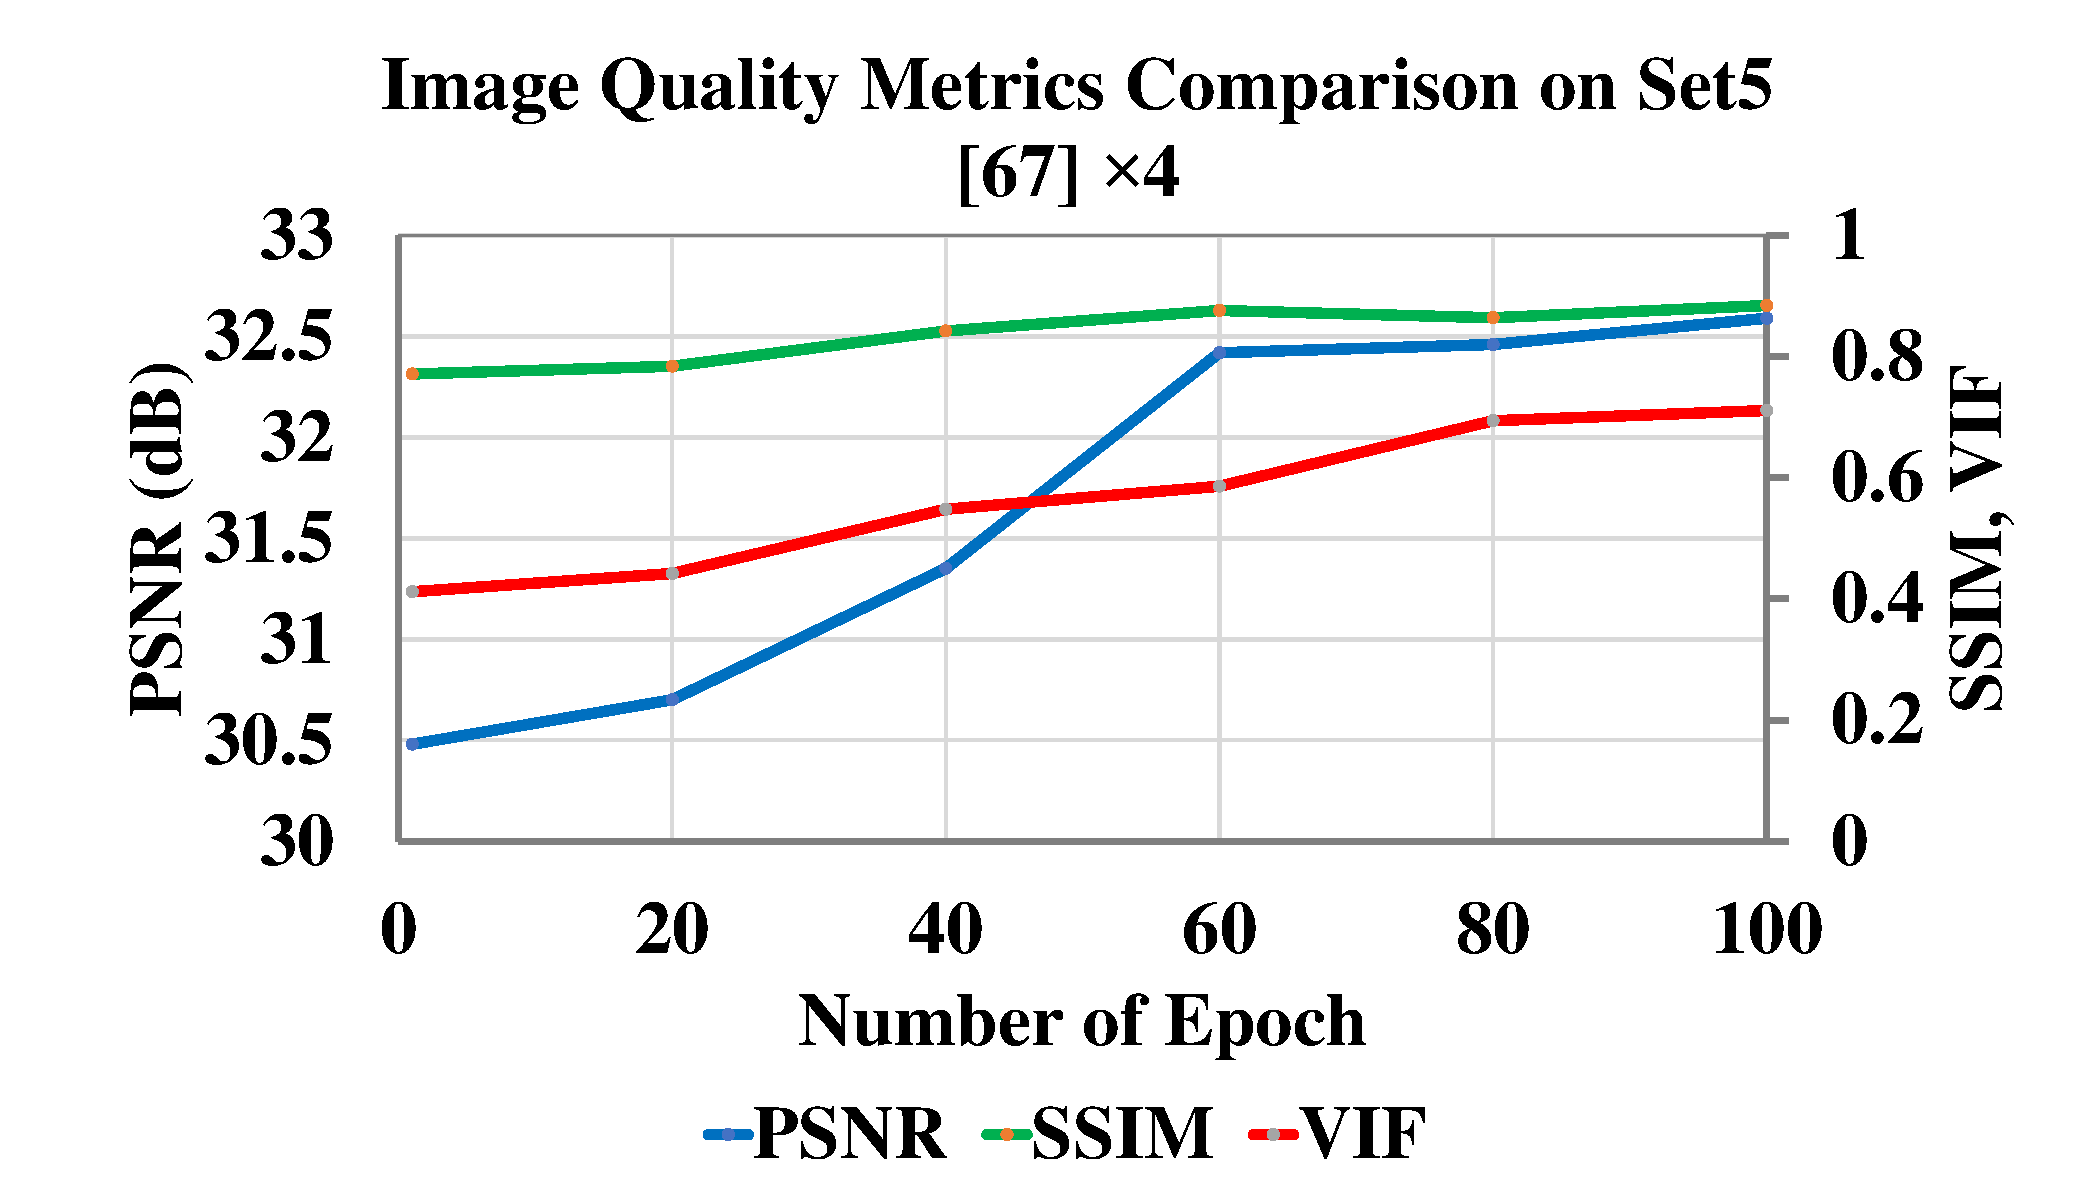
\includegraphics[width=\linewidth]{28FIGURE.pdf}
  \caption{PSNR (dB), SSIM and VIF assessment on Set5 [67] image test dataset for enlargement factor $\times$4.}
  \label{fig:28}
\end{figure}

\begin{table}[ht]
  \centering
  \caption{Quantitative evaluation of our proposed DANS model in terms of  VIFon Set5 [67] test dataset with enlargement factor $\times$4. The best quantitative value has been recorded as bold with {\color{red}\textbf{Red }} color.}

\label{table7}
\setlength{\tabcolsep}{3 pt}
  \begin{tabular}{|c|c|c|} % Specify four columns with "c" for centered alignment

    \hline

   % {Methods} & {Factor} & {VIF}  \\
    \multirow{1}{*}{Methods} & \multirow{1}{*}{Factor} & \multirow{1}{*}{VIF}   \\

    \hline
    SRCNN [17]   & $\times4$   &{0.561}     \\
    FSRCNN [72]   & $\times4$ & {0.613} \\
    VDSR [35]   & $\times4$   & {0.683}   \\
    DANS (Our)  & $\times4$ & {\color{red}\textbf{0.711}}     \\

% Add more rows as needed
    \hline
  \end{tabular}
\end{table}


\section{Discussion}

In the article being discussed, non-local sparse attention (NLSN) and the U-Net framework are combined to propose a novel method for SISR. The model's effectiveness, computational cost, and perceptual quality of the reconstructed high-resolution images are all improved by the adding the inception block, skip connections, and Depth-wise Separable Convolution. Results from comparative evaluations and carefully monitored trials show that the suggested DANS model efficiently enhances the quantitative and perceptual quality of the reconstructed images. The model can effectively capture both local and global information. It is because of the inclusion of non-local sparse attention, which improves reconstruction results when dealing with different up-sampling factors. 

The five benchmark test datasets analysis further demonstrates the DANS model's success in terms of quantitative and qualitative performance measures. The suggested method performs better than current approaches, demonstrating its capacity to produce high-quality reconstructed images under various up-sampling factors. These findings indicate the DANS model's potential as a useful tool for various image improvement applications. One noteworthy feature is the proposed method's reduced computational expense, attained using skip connections and parameter-effective Depth-wise Separable Convolution. The model becomes more computationally efficient without compromising performance by lowering the number of parameters to mitigate the vanishing gradient problem during the training. This is very useful in actual situations with constrained processing resources.

Even though the results presented are encouraging, it is vital to recognize some of the study's limitations. The performance of the DANS model was evaluated using benchmark datasets; however, how well it performs in tough or real-world circumstances is still unknown. Testing the model on a wider variety of photos, especially those with complicated properties or diverse visual content, should be a part of future studies. The authors also provide an overview of their future research goals, which include improving the model for real-time and video super-resolution applications. Using the DANS model in such situations is anticipated to offer insightful information and significantly advance image super-resolution.

Deep Attention Network for SISR (DANS) is a variant of an encoder-decoder network and attention mechanism used in Deep Learning models. This model introduces the concept of the encoder-decoder framework with skip connections and sparsity to reduce computational requirements while improving its performance and encouraging parallelism and scalability in deep learning models. As computational complexity reduces, parallelizing computations over many processors or devices becomes easier. The training and inference procedures may be accelerated, making it easier to deal with larger models or process data in real-time.

DANS can give deep learning models interpretability and explainability, which help to understand the areas that contribute the most to the model's predictions by seeing the attention maps the model produces. These features can help with model debugging, highlighting key components, or understanding how the model makes decisions. It can be applied to various domains and tasks within deep learning, such as natural language processing, computer vision, machine translation, image recognition, and video understanding.


\section{Conclusions and Future Work}

This paper presents a novel fusion of non-local sparse attention NLSN and U-Net framework for single image super-resolution to improve the efficiency and reduce the computational cost of the model. Furthermore, integration of the inception block in the network makes it flexible for the computation of diversified data of the image, which in turn improves the perceptual quality of the image. Additionally, skip connections introduced into the network reduce the parameters used in the network model and ultimately help reduce the model's computational cost. It further helps to reduce the vanishing gradient problem during training. The generalization and convergence of our model are enhanced using Depth-wise Separable Convolution. Depth-wise separable convolution also helps to enhance parameter, computation efficiency and encourages channel-wise feature reuse. Using non-local sparse attention NLSN in the encoder-decoder framework results in efficient local and global modeling. Furthermore, the relative assessment and controlled experiment show the DANS model's effectiveness in improving the reconstructed HR image's quantitative and perceptual quality. A thorough analysis of five benchmark datasets revealed that the proposed DANS model also enhances reconstruction outcomes in terms of quantitative and qualitative norms for up-sampling factors of $\times 2$, $\times 3$, $\times 4$, and $\times 8$. In the future, we will advance our model to introduce real-time and video super-resolution applications under complex scenarios.







\begin{thebibliography}{00}

\bibitem{b1} J. Gupta, S., et al. \textit{Learning rich features from RGB-D images for object detection and segmentation. in European conference on computer vision}. 2014. Springer.

\bibitem{b2} Haris, M., G. Shakhnarovich, and N. Ukita. \textit{Deep back-projection networks for super-resolution}. in \textit{Proceedings of the IEEE conference on computer vision and pattern recognition}. 2018

\bibitem{b3} Zhang, Z., et al. \textit{Facial landmark detection by deep multi-task learning. In European conference on computer vision}. 2014. Springer.

\bibitem{b4} Ronneberger, O., P. Fischer, and T. Brox. \textit{U-net: Convolutional networks for biomedical image segmentation. in International Conference on Medical image computing and computer-assisted intervention}. 2015. Springer.

\bibitem{b5} A. Basharat, A. Gritai, and M. Shah, \textit{"Learning object motion patterns for anomaly detection and improved object detection,"} IEEE Conference on Computer Vision and Pattern Recognition, Anchorage, AK, USA, 2008, pp. 1-8, doi: 10.1109/CVPR.2008.4587510.

\bibitem{b6} Zhang, L., et al., \textit{A super-resolution reconstruction algorithm for surveillance images}. Signal Processing, 2010. 90(3): p. 848-859.

\bibitem{b7} Greenspan, H., \textit{Super-resolution in medical imaging}. The computer journal, 2009. 52(1): p. 43-63

\bibitem{b8} Chen, Y., et al. \textit{Fsrnet: End-to-end learning face super-resolution with facial priors}. in \textit{Proceedings of the IEEE Conference on Computer Vision and Pattern Recognition}. 2018.

\bibitem{b9} Wang, C., et al., \textit{Propagating Facial Prior Knowledge for Multi-Task Learning in Face Super-Resolution}. IEEE Transactions on Circuits and Systems for Video Technology, 2022.

\bibitem{b10} Shakya, S., S. Kumar, and M. Goswami, \textit{Deep learning algorithm for satellite imaging based cyclone detection}. IEEE Journal of Selected Topics in Applied Earth Observations and Remote Sensing, 2020. 13: p. 827-839.

\bibitem{b11} Zhang, H., et al., \textit{Super-resolution reconstruction for multi-angle remote sensing images considering resolution differences}. Remote Sensing, 2014. 6(1): p. 637-657.

\bibitem{b12} Wang, Z., J. Chen, and S.C. Hoi, \textit{Deep learning for image super-resolution: A survey}. IEEE transactions on pattern analysis and machine intelligence, 2020. 43(10): p. 3365- 3387.

\bibitem{b13} Barla, N. \textit{A Gentle introduction to Deep Learning-the ELI5 Way}. 2022 5/08/2022]; Available from:

\bibitem{b14} Muhammad, Wazir, Supavadee Aramvith, and Takao Onoye. \textit{"SENext: Squeeze-and-ExcitationNext for Single Image Super-Resolution." }IEEE Access (2023).

\bibitem{b15} Hajian, A. and Aramvith, S.,  \textit{Fusion Objective Function on Progressive Super-Resolution Network}. Journal of Sensor and Actuator Networks, 2023. 12(2), p.26.

\bibitem{b16} Ruangsang, Watchara, Supavadee Aramvith, and Takao Onoye. "Multi-FusNet of Cross Channel Network for Image Super-Resolution." IEEE Access (2023).

\bibitem{b17} C. Dong, C. C. Loy, K. He and X. Tang, \textit{"Image super-resolution using deep convolutional networks"}, \textit{IEEE Trans. Pattern Anal. Mach. Intell.}, vol. 38, pp. 295-307, Feb. 2015.

\bibitem{b18} Ledig, C., et al. \textit{Photo-realistic single image super-resolution using a generative adversarial network}. in \textit{Proceedings of the IEEE conference on computer vision and pattern recognition}. 2017.

\bibitem{b19} Zhang, Y., et al. \textit{Image super-resolution using very deep residual channel attention networks}. in \textit{Proceedings of the European conference on computer vision (ECCV)}. 2018.

\bibitem{b20} Kim, J.-H., et al., \textit{Ram: Residual attention module for single image super-resolution}. arXiv preprint arXiv:1811.12043, 2018. 2(1): p. 2.

\bibitem{b21} Yu, X. and F. Porikli. \textit{Face hallucination with tiny unaligned images by transformative discriminative neural networks}. in \textit{Proceedings of the AAAI Conference on Artificial Intelligence}. 2017.

\bibitem{b22} Lim, B., et al. \textit{Enhanced deep residual networks for single image super-resolution}. in \textit{Proceedings of the IEEE conference on computer vision and pattern recognition workshops}. 2017

\bibitem{b23} Huang, H., et al. \textit{Wavelet-srnet: A wavelet-based cnn for multi-scale face super-resolution}. in \textit{Proceedings of the IEEE International Conference on Computer Vision}. 2017.

\bibitem{b24} Guo, T., et al. \textit{Deep wavelet prediction for image super-resolution}. in \textit{Proceedings of the IEEE conference on computer vision and pattern recognition workshops}. 2017.

\bibitem{b25} Fan, Y., et al., \textit{Neural sparse representation for image restoration}. Advances in Neural Information Processing Systems, 2020. 33: p. 15394-15404.

\bibitem{b26} Yang, J., et al., \textit{Image super-resolution via sparse representation}. IEEE transactions on image processing, 2010. 19(11): p. 2861-2873.

\bibitem{b27} Wang, Z., et al. \textit{Deep networks for image super-resolution with sparse prior}. in \textit{Proceedings of the IEEE international conference on computer vision}. 2015.

\bibitem{b28} Kim, K.I. and Y. Kwon, \textit{Single-image super-resolution using sparse regression and natural image prior}. IEEE transactions on pattern analysis and machine intelligence, 2010. 32(6): p. 1127-1133.

\bibitem{b29} Wang, X., Girshick, R., Gupta, A. and He, K. \textit{Non-local neural networks}. In Proceedings of the IEEE conference on computer vision and pattern recognition, 2018. (pp. 7794-7803).

\bibitem{b30} Mei, Y., Y. Fan, and Y. Zhou. \textit{Image super-resolution with non-local sparse attention}. in \textit{Proceedings of the IEEE/CVF Conference on Computer Vision and Pattern Recognition}. 2021.

\bibitem{b31} Isola, P., Zhu, J.Y., Zhou, T. and Efros, A.A., \textit{Image-to-image translation with conditional adversarial networks}. In \textit{Proceedings of the IEEE conference on computer vision and pattern recognition}, 2017.  (pp. 1125-1134).

\bibitem{b32} Mao, X., C. Shen, and Y.-B. Yang, \textit{Image restoration using deep convolutional encoder-decoder networks with symmetric skip connections}. Advances in neural information processing systems, 2016. 29.

\bibitem{b33} Tong, T., et al. \textit{Image super-resolution using dense skip connections}. in \textit{Proceedings of the IEEE international conference on computer vision}. 2017.

\bibitem{b34} J. Yamanaka, S. Kuwashima and T. Kurita, \textit{"Fast and accurate image super-resolution by deep cnn with skip connection and network in network"}, \textit{Proc. ICNIP}, pp. 217-225, 2017.

\bibitem{b35} J. Kim, J. K. Lee and K. M. Lee, \textit{"Accurate image super-resolution using very deep convolutional networks"}, \textit{Proc. IEEE Conf. Comput. Vis. Pattern Recognit.}, pp. 1646-1654, Jun. 2016

\bibitem{b36} Kim, J., J.K. Lee, and K.M. Lee. \textit{Deeply-recursive convolutional network for image super-resolution}. in \textit{Proceedings of the IEEE conference on computer vision and pattern recognition}. 2016.

\bibitem{b37} Jiang, J., Zheng, L., Luo, F. and Zhang, Z., \textit{Rednet: Residual encoder-decoder network for indoor rgb-d semantic segmentation}, 2018. arXiv preprint arXiv:1806.01054.

\bibitem{b38} Chen, J. and Li, F., \textit{Denoising convolutional neural network with mask for salt and pepper noise}. IET Image Processing, 2019. 13(13), pp.2604-2613.

\bibitem{b39} Hui, Z., Gao, X., Yang, Y. and Wang, X., \textit{Lightweight image super-resolution with information multi-distillation network}. In \textit{Proceedings of the 27th ACM international conference on multimedia}, October 2019. (pp. 2024-2032).

\bibitem{b40} N. Ahn, B. Kang and K.-A. Sohn, \textit{"Fast accurate and lightweight super-resolution with cascading residual network"}, \textit{ Proceedings of the European conference on computer vision (ECCV)}, pp. 252-268, 2018.

\bibitem{b41} J.-H. Choi, J.-H. Kim, M. Cheon and J.-S. Lee, \textit{"Lightweight and efficient image super-resolution with block state-based recursive network"},\textit{arXiv:1811.12546}, 2018, [online] Available: http://arxiv.org/abs/1811.12546.

\bibitem{b42} Tai, Y., Yang, J. and Liu, X., \textit{Image super-resolution via deep recursive residual network}. In \textit{Proceedings of the IEEE conference on computer vision and pattern recognition}, 2017. (pp. 3147-3155).

\bibitem{b43} Y. Tai, J. Yang, X. Liu and C. Xu, \textit{"MemNet: A persistent memory network for image restoration"}, \textit{Proc. IEEE Conf. Int. Conf. Comput. Vis.}, Oct 2017. pp. 4539-4547. 

\bibitem{b44} J. Li, F. Fang, K. Mei and G. Zhang, \textit{"Multi-scale residual network for image super-resolution"}, \textit{Proc. Eur. Conf. Comput. Vis. (ECCV)}, Sep 2018. pp. 517-532.

\bibitem{b45} K. Zhang, W. Zuo and L. Zhang, \textit{"Learning a single convolutional super-resolution network for multiple degradations}", \textit{Proc. IEEE/CVF Conf. Comput. Vis. Pattern Recognit.}, Jun. 2018. vol. 6, no. 1, pp. 3262-3271.

\bibitem{b46} X. Yang, H. Mei, J. Zhang, K. Xu, B. Yin, Q. Zhang, et al., \textit{"DRFN: Deep recurrent fusion network for single-image super-resolution with large factors"}, \textit{IEEE Trans. Multimedia}, Feb. 2019. vol. 21, no. 2, pp. 328-337.

\bibitem{b47} K.-W. Hung, Z. Zhang and J. Jiang, \textit{"Real-time image super-resolution using recursive depthwise separable convolution network"}, \textit{IEEE Access}, vol. 7, pp. 99804-99816, 2019.

\bibitem{b48} Z. Hui, X. Wang and X. Gao, \textit{"Fast and accurate single image super-resolution via information distillation network"}, \textit{Proc. IEEE/CVF Conf. Comput. Vis. Pattern Recognit.}, pp. 723-731, Jun. 2018.

\bibitem{b49} Mei, Y., et al. \textit{Image super-resolution with cross-scale non-local attention and exhaustive self-exemplars mining}. in \textit{Proceedings of the IEEE/CVF conference on computer vision and pattern recognition}. 2020.

\bibitem{b50} Niu, B., Wen, W., Ren, W., Zhang, X., Yang, L., Wang, S., Zhang, K., Cao, X. and Shen, H., 2020. \textit{Single image super-resolution via a holistic attention network}. In \textit{Computer Vision–ECCV 2020: 16th European Conference, Glasgow, UK, August 23–28, 2020, Proceedings, Part XII 16} (pp. 191-207). Springer International Publishing.

\bibitem{b51} Dai, T., et al. \textit{Second-order attention network for single image super-resolution}. in \textit{Proceedings of the IEEE/CVF conference on computer vision and pattern recognition}. 2019.

\bibitem{b52} Anwar, S. and N. Barnes, \textit{Densely residual laplacian super-resolution}. IEEE Transactions on Pattern Analysis and Machine Intelligence, 2020.

\bibitem{b53} Zhang, X., Zeng, H., Guo, S. and Zhang, L., 2022, October. \textit{Efficient long-range attention network for image super-resolution}. In \textit{Computer Vision–ECCV 2022: 17th European Conference, Tel Aviv, Israel,} October 23–27, 2022, Proceedings, Part XVII (pp. 649-667). Cham: Springer Nature Switzerland.

\bibitem{b54} Lu, E., Hu, X. \textit{Image super-resolution via channel attention and spatial attention.} Appl Intell 52, 2260–2268 (2022). https://doi.org/10.1007/s10489-021-02464-6.


\bibitem{b55} Liu, J., et al. \textit{Residual feature aggregation network for image super-resolution}. in \textit{Proceedings of the IEEE/CVF conference on computer vision and pattern recognition}. 2020.

\bibitem{b56} Zhang, Y., et al., \textit{Residual non-local attention networks for image restoration}. arXiv preprint arXiv:1903.10082, 2019.

\bibitem{b57} Z. Wang, D. Liu, Z. Wang, J. Yang and T. Huang, \textit{"Deeply improved sparse coding for image super-resolution"}, \textit{Proc. IEEE Int. Conf. Comput. Vis.}, pp. 370-378, Dec. 2015.

\bibitem{b58} Chang, H., D.-Y. Yeung, and Y. Xiong. \textit{Super-resolution through neighbor embedding}. in \textit{Proceedings of the 2004 IEEE Computer Society Conference on Computer Vision and Pattern Recognition, 2004. CVPR 2004}. 2004. IEEE.

\bibitem{b59} Yang, J., et al. \textit{Image super-resolution as sparse representation of raw image patches}. in \textit{2008 IEEE conference on computer vision and pattern recognition}. 2008. IEEE.

\bibitem{b60} C. Szegedy, W. Liu, Y. Jia, P. Sermanet, S. Reed, D. Anguelov, D. Erhan, V. Vanhoucke, and A. Rabinovich. \textit{Going deeper with convolutions}. In Proceedings of the IEEE Conference on Computer Vision and Pattern Recognition, pages 1–9, 2015

\bibitem{b61} R. Wang, M. Gong and D. Tao, \textit{"Receptive field size versus model depth for single image super-resolution"}, \textit{IEEE Trans. Image Process.}, vol. 29, pp. 1669-1682, 2019.

\bibitem{b62} Keys, R., \textit{Cubic convolution interpolation for digital image processing}. IEEE transactions on Acoustics, speech, and signal processing, 1981. 29(6): p. 1153-1160.

\bibitem{b63} M. Su, S. Lai, Z. Chai, X. Wei, and Y. Liu, \textit{"Hierarchical Recursive Network for Single Image Super-Resolution"},\textit{IEEE International Conference on Multimedia \& Expo Workshops (ICMEW)}, pp. 595-598, 2019.

\bibitem{b64} Park, S.-J., et al. \textit{Srfeat: Single image super-resolution with feature discrimination}. in \textit{Proceedings of the European conference on computer vision (ECCV)}. 2018.

\bibitem{b65} Kaiming He, Xiangyu Zhang, Shaoqing Ren, Jian Sun. \textit{"Delving Deep into Rectifiers: Surpassing Human-Level Performance on ImageNet Classification}.\textit{" In Proceedings of the IEEE International Conference on Computer Vision (ICCV)}, 2015

\bibitem{b66} Agustsson, E.,  Timofte, R. \textit{"NTIRE 2017 Challenge on Single Image Super-Resolution: Dataset and Study."} IEEE Conference on Computer Vision and Pattern Recognition Workshops (CVPRW), (2017). 126-135.

\bibitem{b67} Bevilacqua, M.; Roumy, A.; Guillemot, C.; Alberi-Morel, M.L. \textit{Low-complexity single-image super-resolution based on nonnegative neighbor embedding}. In \textit{Proceedings of the British Machine Vision Conference, Surrey}, UK, 3–7 September 2012.

\bibitem{b68} Zeyde, R.; Elad, M.; Protter, M. \textit{On Single Image Scale-Up Using Sparse-Representations}. In \textit{Proceedings of the International Conference on Curves and Surfaces}, Oslo, Norway, 28 June–3 July 2012; pp. 711–730.

\bibitem{b69} Martin, D.; Fowlkes, C.; Tal, D.; Malik, J. \textit{A database of human segmented natural images and its application to evaluating segmentation algorithms and measuring ecological statistics}. In \textit{Proceedings of the Eighth International Conference On Computer Vision} (ICCV-01), Vancouver, BC, Canada, 7–14 July 2001.

\bibitem{b70} Huang, J.-B.; Singh, A.; Ahuja, N. \textit{Single image super-resolution from transformed self-exemplars}. In \textit{Proceedings of the IEEE Conference on Computer Vision and Pattern Recognition}, Boston, MA, USA, 7–12 June 2015.

\bibitem{b71} Matsui, Y.; Ito, K.; Aramaki, Y.; Fujimoto, A.; Ogawa, T.; Yamasaki, T.; Aizawa, K. \textit{Sketch-based manga retrieval using manga109 dataset}. Multimedia. Tools Appl. 2017, 76, 21811–21838 

\bibitem{b72} Dong, C., C.C. Loy, and X. Tang. \textit{Accelerating the super-resolution convolutional neural network. in European conference on computer vision}. 2016. Springer.

\bibitem{b73} Zhang, Y., et al. \textit{Residual dense network for image super-resolution}. in \textit{Proceedings of the IEEE conference on computer vision and pattern recognition}. 2018.

\bibitem{b74} W.-S. Lai, J.-B. Huang, N. Ahuja and M.-H. Yang, \textit{"Deep Laplacian pyramid networks for fast and accurate super-resolution"}, \textit{Proc. IEEE Conf. Comput. Vis. Pattern Recognit.}, pp. 5835-5843, Jul. 2017.

\bibitem{b75} Ai W, Tu X, Cheng S, Xie M. \textit{Single image super-resolution via residual neuron attention networks}. In \textit{IEEE International Conference on Image Processing (ICIP) 2020 Oct 25 (pp. 1586-1590)}. IEEE.

\bibitem{b76} Li, Z., et al. \textit{Feedback network for image super-resolution}. in \textit{Proceedings of the IEEE/CVF conference on computer vision and pattern recognition}. 2019.

\bibitem{b77} Liang, J., Cao, J., Sun, G., Zhang, K., Van Gool, L. and Timofte, R. \textit{Swinir: Image restoration using swin transformer}. In \textit{Proceedings of the IEEE/CVF international conference on computer vision}, 2021. (pp. 1833-1844).

\bibitem{b78} Wang, C., Li, Z. and Shi, J., \textit{Lightweight image super-resolution with adaptive weighted learning network}, 2019. arXiv preprint arXiv:1904.02358.

\bibitem{b79} Zhang, K., et al. \textit{Learning deep CNN denoiser prior for image restoration}. in \textit{Proceedings of the IEEE conference on computer vision and pattern recognition}. 2017.

\bibitem{b80} Frome, A. and J. Malik, 10 \textit{Object Recognition Using Locality-Sensitive Hashing of Shape Contexts}. Nearest-neighbour methods in learning and vision: theory and practice, 2005: p.221. 

\bibitem{b81} Dabov, K., Foi, A., Katkovnik, V. and Egiazarian, K. \textit{Color image denoising via sparse 3D collaborative filtering with grouping constraint in luminance-chrominance space.} In 2007 IEEE international conference on image processing, September 2007. (Vol. 1, pp. I-313). IEEE.

\bibitem{b82} Gu, S., Zhang, L., Zuo, W. and Feng, X. \textit{Weighted nuclear norm minimization with application to image denoising}. In Proceedings of the IEEE conference on computer vision and pattern recognition, 2014. (pp. 2862-2869).

\bibitem{b83} Zhang, K., Zuo, W. and Zhang, L., 2018. \textit{FFDNet: Toward a fast and flexible solution for CNN-based image denoising.} IEEE Transactions on Image Processing, 27(9), pp.4608-4622.

\bibitem{b84} Dong, W., Zhang, L., Shi, G. and Li, X. \textit{Nonlocally centralized sparse representation for image restoration.} IEEE Transactions on Image Processing, 22(4),  2012. pp.1620-1630.


\end{thebibliography}

\begin{IEEEbiography}[{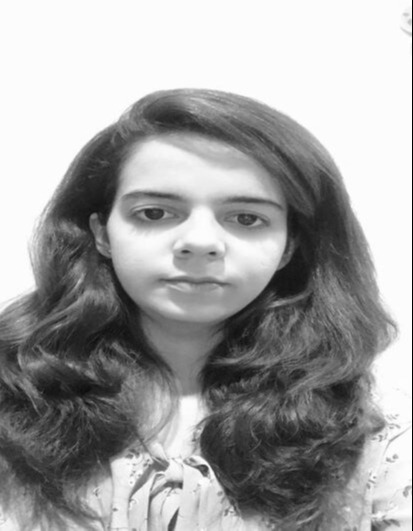
\includegraphics[width=1in,height=1.25in,clip,keepaspectratio]{a.png}}]{Jagrati Talreja} (Graduate Student Member, IEEE) received the B.TECH. in Electronics and Communication Engineering Networks from Pranveer Singh Institute of Technology, Kanpur, Uttar Pradesh, India in 2019. Ms Jagrati is pursuing her 5-year continuing doctoral degree from the Department of Electrical Engineering Chulalongkorn University Bangkok, Thailand from 2019 to 2024. Her research interests lie in Electrical Engineering, Neural Networks, and Machine Learning, specifically in Deep Learning image super-resolution.

\end{IEEEbiography}

\begin{IEEEbiography}[{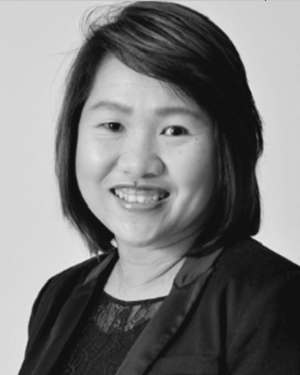
\includegraphics[width=1in,height=1.25in,clip,keepaspectratio]{b.png}}]{SUPAVADEE ARAMVITH} (Senior Member, IEEE) received the B.S. degree (Hons.) in computer science from Mahidol University, in 1993, and the M.S. and Ph.D. degrees in electrical engineering from the University of Washington, Seattle, USA, in 1996 and 2001, respectively. In June 2001, she joined Chulalongkorn University, where she is currently an Associate Professor at the Department of Electrical Engineering, specializing in video technology. She has successfully advised 32 bachelor’s, 27 master’s, and 10 Ph.D. graduates. She published over 130 articles in international conference proceedings and journals with four international book chapters. She has rich project management experiences as a project leader and a former technical committee chairs to the Thailand Government bodies in Telecommunications and ICT. She is very active in the international arena with the leadership positions in the international network such as JICA Project for AUN/SEEDNet, and the professional organizations, such as the IEEE, IEICE, APSIPA, and ITU.
\end{IEEEbiography}

\begin{IEEEbiography}[{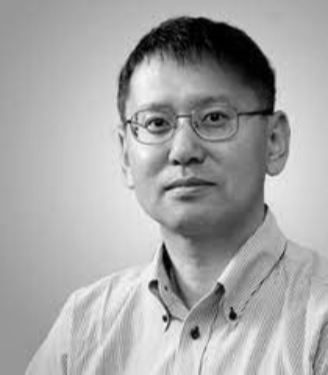
\includegraphics[width=1in,height=1.25in,clip,keepaspectratio]{c.png}}]{Takao Onoye} (Senior Member, IEEE) received the B.E. and M.E. degrees in electronic engineering and the Dr.Eng. degree in information systems engineering from Osaka University, Osaka, Japan, in 1991, 1993, and 1997, respectively. He was an Associate Professor with the Department of Communications and Computer Engineering, Kyoto University, Kyoto, Japan. Since 2003, he has been a Professor with the Department of Information Systems Engineering, Osaka University. He has published over 200 research papers in VLSI design and multimedia signal processing in reputed journals and proceedings of international conferences. His research interests include media-centric low-power architecture and its SoC implementation. Dr. Onoye has been served as a member of the CAS Society Board of Governors, since 2008. He is also a member of IEICE, IPSJ, and ITE-J.


\end{IEEEbiography}



\EOD

\end{document}
